% Se pre-carga la información del estudiante sólo para poder emplear el macro de
% selección de versión (digital o impresa)
% ===============================================================================
% El estudiante debe llenar sus datos en esta sección para que la plantilla los 
% auto-importe y genere automáticamente las páginas de portada y de firmas 
% autorizadas.
% ===============================================================================
% Datos del estudiante:
% -------------------------------------------------------------------------------
% Nombre completo
\def \nombreestudiante {Gerardo Paz Fuentes}
% Carné
\def \uvgcarne {20173}
% Facultad
\def \uvgfacultad {Ingeniería}
% Carrera
\def \uvgcarrera {Ingeniería Mecatrónica}

% Datos del trabajo:
% -------------------------------------------------------------------------------
% Título completo
\def \titulotesis {
	Optimización de un algoritmo de inteligencia de enjambre enfocado en sincronización y control de formaciones de sistemas robóticos multi-agente para escenarios con obstáculos móviles
}
% Año de entrega
\def \anoentrega {2024}
% Asesor
\def \nombreasesor {Dr. Luis Rivera}

% Datos del tribunal examinador:
% -------------------------------------------------------------------------------
% Nombre del primer examinador
\def \nombreprimerex {Examinador 1}
% Nombre del segundo examinador
\def \nombresegundoex {Examinador 2}
% Año de aprobación
\def \anoaprobacion {2024}
% Mes de aprobación
\def \mesaprobacion {diciembre }
% Día de aprobación
\def \diaaprobacion {5 }

% Capítulos pre-definidos
% -------------------------------------------------------------------------------
% Comentar las líneas de las secciones que desean omitirse, por defecto se 
% se incluyen todas.
\def \CAPprefacio {Prefacio}
\def \CAPantecedentes {Antecedentes}
\def \CAPalcance {Alcance}
\def \CAPanexos {Anexos}
\def \CAPglosario {Glosario}

% Formato y estilo de la plantilla
% -------------------------------------------------------------------------------
% Modo impresión: Puede des-comentar la siguiente línea para generar un documento pdf sin la portada, para cuando se desee imprimir el documento para encuadernación
%\def \printver {Versión del documento para impresión}

% Portada: Puede cambiarse la imagen en la portada al cambiar el nombre del 
% archivo siguiente. NOTA: debe tener la suficiente resolución para cubrir el área
% designada
\def \imagenportada {plantilla/portadacit.jpg}

% Referencias: Puede des-comentar la siguiente línea para utilizar el formato de referencias APA
%\def \usarAPA {Usar formato APA}

% Párrafo: Puede comentar la siguiente línea si desea emplear un formato de 
% párrafo distinto al establecido por defecto
\def \parpordefecto {Formato de párrafo por defecto}

% Capítulos y secciones: Puede des-comentar la siguiente línea para establecer el
% formato de los capítulos y secciones bajo el estándar original de UVG para
% trabajos de graduación. Este incluye: capítulos con numeración romana, secciones
% con letras mayúsculas, sub-secciones con números y sub-sub-secciones con letras
% minúsculas
%\def \capsecuvg {Formato UVG para capítulos y secciones}

\ifdefined\printver
    \documentclass[11pt, letterpaper, twoside, openright]{report}
\else
    \documentclass[11pt, letterpaper]{report}
\fi

% Eliminar la opción de twoside y openright si se desea generar la versión
% digital del documento en lugar de la versión impresa
%\documentclass[11pt, letterpaper, twoside, openright]{report}
\usepackage[spanish, es-nodecimaldot, es-noquoting]{babel}
% cambiar a spanish, mexico si se quiere emplear tabla en lugar de cuadro
\selectlanguage{spanish}
\usepackage[utf8]{inputenc}
\usepackage[T1]{fontenc}

\title{Plantilla para Trabajos de Graduación IE-MT 2019v4}
\author{MSc. Miguel Zea}
\date{\today}

% Información del estudiante en el archivo datos_estudiante.tex
% ===============================================================================
% El estudiante debe llenar sus datos en esta sección para que la plantilla los 
% auto-importe y genere automáticamente las páginas de portada y de firmas 
% autorizadas.
% ===============================================================================
% Datos del estudiante:
% -------------------------------------------------------------------------------
% Nombre completo
\def \nombreestudiante {Gerardo Paz Fuentes}
% Carné
\def \uvgcarne {20173}
% Facultad
\def \uvgfacultad {Ingeniería}
% Carrera
\def \uvgcarrera {Ingeniería Mecatrónica}

% Datos del trabajo:
% -------------------------------------------------------------------------------
% Título completo
\def \titulotesis {
	Optimización de un algoritmo de inteligencia de enjambre enfocado en sincronización y control de formaciones de sistemas robóticos multi-agente para escenarios con obstáculos móviles
}
% Año de entrega
\def \anoentrega {2024}
% Asesor
\def \nombreasesor {Dr. Luis Rivera}

% Datos del tribunal examinador:
% -------------------------------------------------------------------------------
% Nombre del primer examinador
\def \nombreprimerex {Examinador 1}
% Nombre del segundo examinador
\def \nombresegundoex {Examinador 2}
% Año de aprobación
\def \anoaprobacion {2024}
% Mes de aprobación
\def \mesaprobacion {diciembre }
% Día de aprobación
\def \diaaprobacion {5 }

% Capítulos pre-definidos
% -------------------------------------------------------------------------------
% Comentar las líneas de las secciones que desean omitirse, por defecto se 
% se incluyen todas.
\def \CAPprefacio {Prefacio}
\def \CAPantecedentes {Antecedentes}
\def \CAPalcance {Alcance}
\def \CAPanexos {Anexos}
\def \CAPglosario {Glosario}

% Formato y estilo de la plantilla
% -------------------------------------------------------------------------------
% Modo impresión: Puede des-comentar la siguiente línea para generar un documento pdf sin la portada, para cuando se desee imprimir el documento para encuadernación
%\def \printver {Versión del documento para impresión}

% Portada: Puede cambiarse la imagen en la portada al cambiar el nombre del 
% archivo siguiente. NOTA: debe tener la suficiente resolución para cubrir el área
% designada
\def \imagenportada {plantilla/portadacit.jpg}

% Referencias: Puede des-comentar la siguiente línea para utilizar el formato de referencias APA
%\def \usarAPA {Usar formato APA}

% Párrafo: Puede comentar la siguiente línea si desea emplear un formato de 
% párrafo distinto al establecido por defecto
\def \parpordefecto {Formato de párrafo por defecto}

% Capítulos y secciones: Puede des-comentar la siguiente línea para establecer el
% formato de los capítulos y secciones bajo el estándar original de UVG para
% trabajos de graduación. Este incluye: capítulos con numeración romana, secciones
% con letras mayúsculas, sub-secciones con números y sub-sub-secciones con letras
% minúsculas
%\def \capsecuvg {Formato UVG para capítulos y secciones}
% ================================================================================
% En este archivo se colocan opciones adicionales para modificar el formato de la
% plantilla, para emplearse en otros tipos de documentos que no sean trabajos de
% graduación. Si usted está trabajando su tesis, NO modifique este archivo
% ================================================================================
% Capítulos pre-definidos
% --------------------------------------------------------------------------------
% Comentar las líneas de las secciones que desean omitirse, por defecto se 
% se incluyen todas.
\def \CAPportada {Portada}
\def \CAPcaratula {Caratula}
\def \CAPfirmas {Hoja de firmas}
\def \CAPindice {Índice general}
\def \CAPfiguras {Listado de figuras}
\def \CAPcuadros {Listado de cuadros}
\def \CAPresumen {Resumen}
\def \CAPabstract {Resumen}
\def \CAPintroduccion {Introducción}
\def \CAPobjetivos {Objetivos}
\def \CAPjustificacion {Justificación}
\def \CAPmarcoteorico {Marco teórico}
\def \CAPconclusiones {Conclusiones}
\def \CAPrecomendaciones {Recomendaciones}
\def \CAPbibliografia {Bibliografía}

% ==============================================================================
% DEFINICIÓN DE PAQUETES
% ==============================================================================
\usepackage{multirow}
\usepackage{xcolor}
\usepackage{amsfonts}
\usepackage{amsmath}
\usepackage{amssymb}
\usepackage{amsthm}
\usepackage{amsfonts}
\usepackage{mathtools}
\usepackage{graphicx}
\usepackage{xfrac}
\usepackage{float}
\usepackage{mathtools}
\usepackage[hypertexnames=false]{hyperref}
% \usepackage{bookmark}
\usepackage[font=small]{caption}
\usepackage{subcaption}
%\usepackage{csquotes}
\usepackage{xpatch}
\usepackage{emptypage}
\usepackage{hyphenat}
\usepackage{fancyhdr}
\usepackage[backend=biber, style=ieee]{biblatex}
\ifdefined\usarAPA 
    \usepackage[backend=biber, style=apa]{biblatex}
\fi
\addbibresource{m-bibliografia.bib}

\usepackage[percent]{overpic}

\usepackage{chngcntr}

\ifdefined\CAPglosario
	%\usepackage[toc]{glossaries}
	\usepackage[numberedsection]{glossaries}
	\makeglossaries
    \newglossaryentry{latex}
{
    name=latex,
    description={Es un lenguaje de marcado adecuado especialmente para la creación de documentos científicos}
} 
 
\newglossaryentry{formula}
{
    name=fórmula,
    description={Una expresión matemática} 
}
\fi

% ==============================================================================
% MÁRGENES Y FORMATO GENERALES
% ==============================================================================
\usepackage[top=1in, left=1.5in, right=1in, bottom=1in]{geometry}
%Options: Sonny, Lenny, Glenn, Conny, Rejne, Bjarne, Bjornstrup
\usepackage[Sonny]{fncychap}

% ==============================================================================
% DEFINICIONES DE LA PLANTILLA
% ==============================================================================
\graphicspath{ {figuras/} }
\definecolor{uvg-green}{RGB}{17,71,52}
\newcommand{\defaultparformat}[1]{
	{\setlength{\parskip}{2ex}
     \input{#1}}
}
\ifdefined\capsecuvg
	\renewcommand\thechapter{\Roman{chapter}}
    \renewcommand\thesection{\Alph{section}}
	\renewcommand\thesubsection{\arabic{subsection}}
    \renewcommand\thesubsubsection{\alph{subsubection}}
\fi
\counterwithout{figure}{chapter}
\counterwithout{table}{chapter}
\counterwithout{equation}{chapter}

\newcommand{\blankpage}{
\newpage
\thispagestyle{empty}
\mbox{}
\newpage
}
% ==============================================================================

% Comandos definidos por el usuario en el archivo comandos_usuario.tex
\input{2-paquetes_y_comandos_usuario}

% ==============================================================================
% CUERPO DEL TRABAJO
% ==============================================================================
\pagestyle{headings}
\begin{document}

% ==============================================================================
% PORTADA
% ==============================================================================
\ifdefined\printver
    \let\CAPportada\undefined
\fi 

\ifdefined\CAPportada
    \cleardoublepage\phantomsection
    % \pdfbookmark{Portada}{toc}
	\newgeometry{left=3cm, bottom=0in, top=1in, right=3cm}
	\pagecolor{uvg-green}
	\thispagestyle{empty}

	\color{white}
	\noindent \hrulefill \par
	\vspace{0.1in}
	\noindent \Huge \nohyphens{\titulotesis} \par
	\noindent \hrulefill \par
	\noindent
	\LARGE \nombreestudiante

	\begin{figure}[b!]
    	%\makebox[\textwidth]{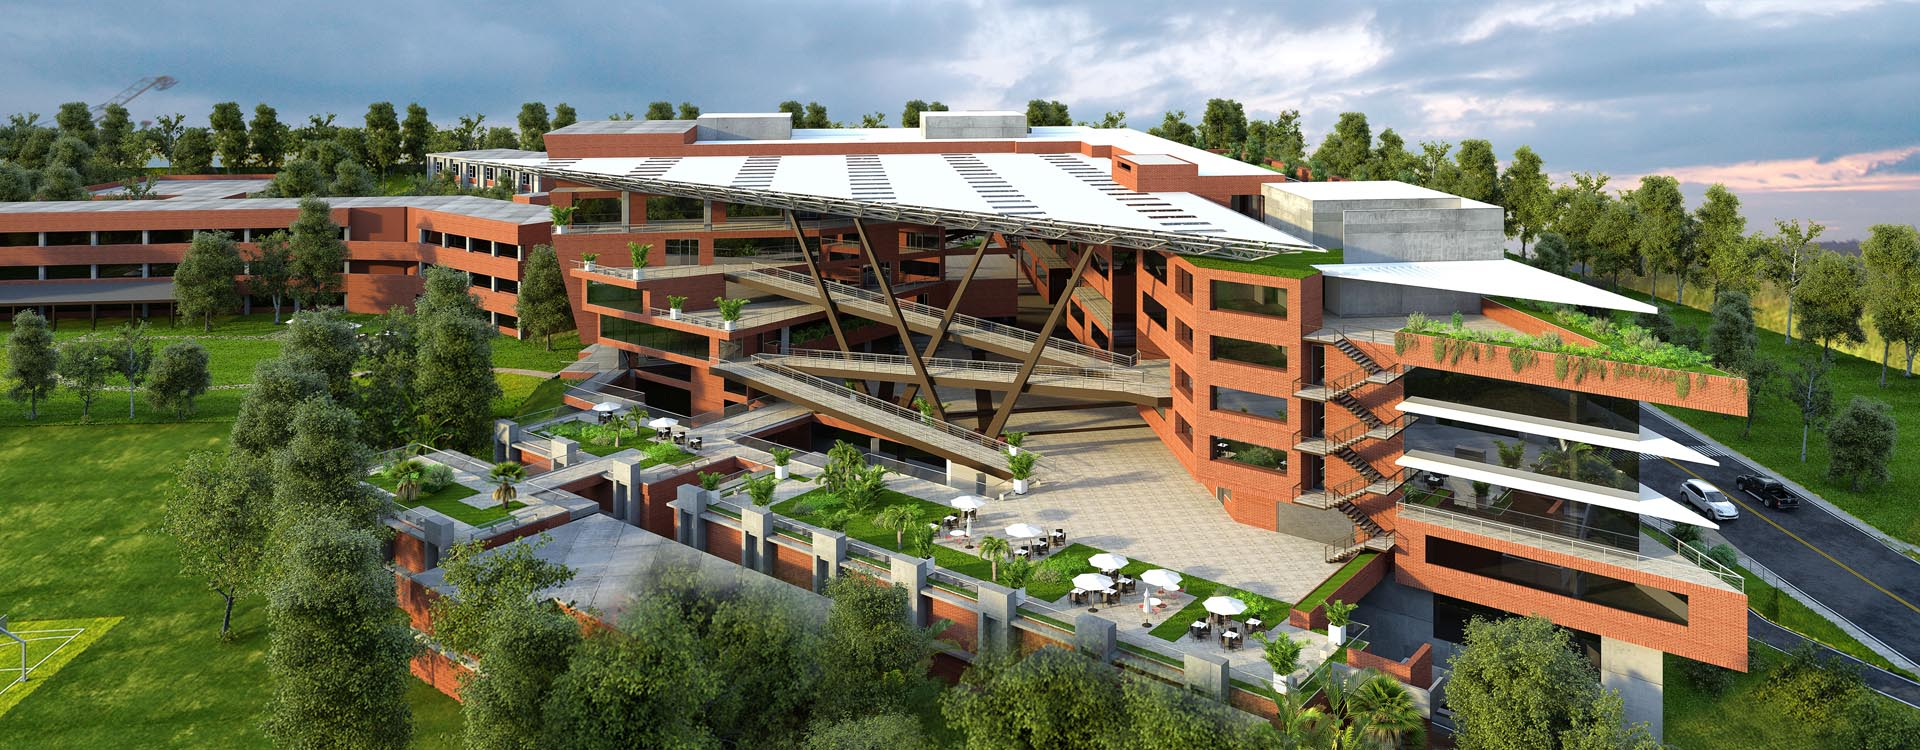
\includegraphics[height=13.25cm]{plantilla/portadacit.jpg}}
    	\makebox[\textwidth]{
    		\begin{overpic}[height=13.25cm]{\imagenportada}
     		\put(63,0){
\includegraphics[height=1.15in]{plantilla/fondologo_grande.png}}  
  			\put(64.5,2){
\includegraphics[height=0.55in]{plantilla/logoUVGblanco.eps}} 
        	\end{overpic}
    	}
    	%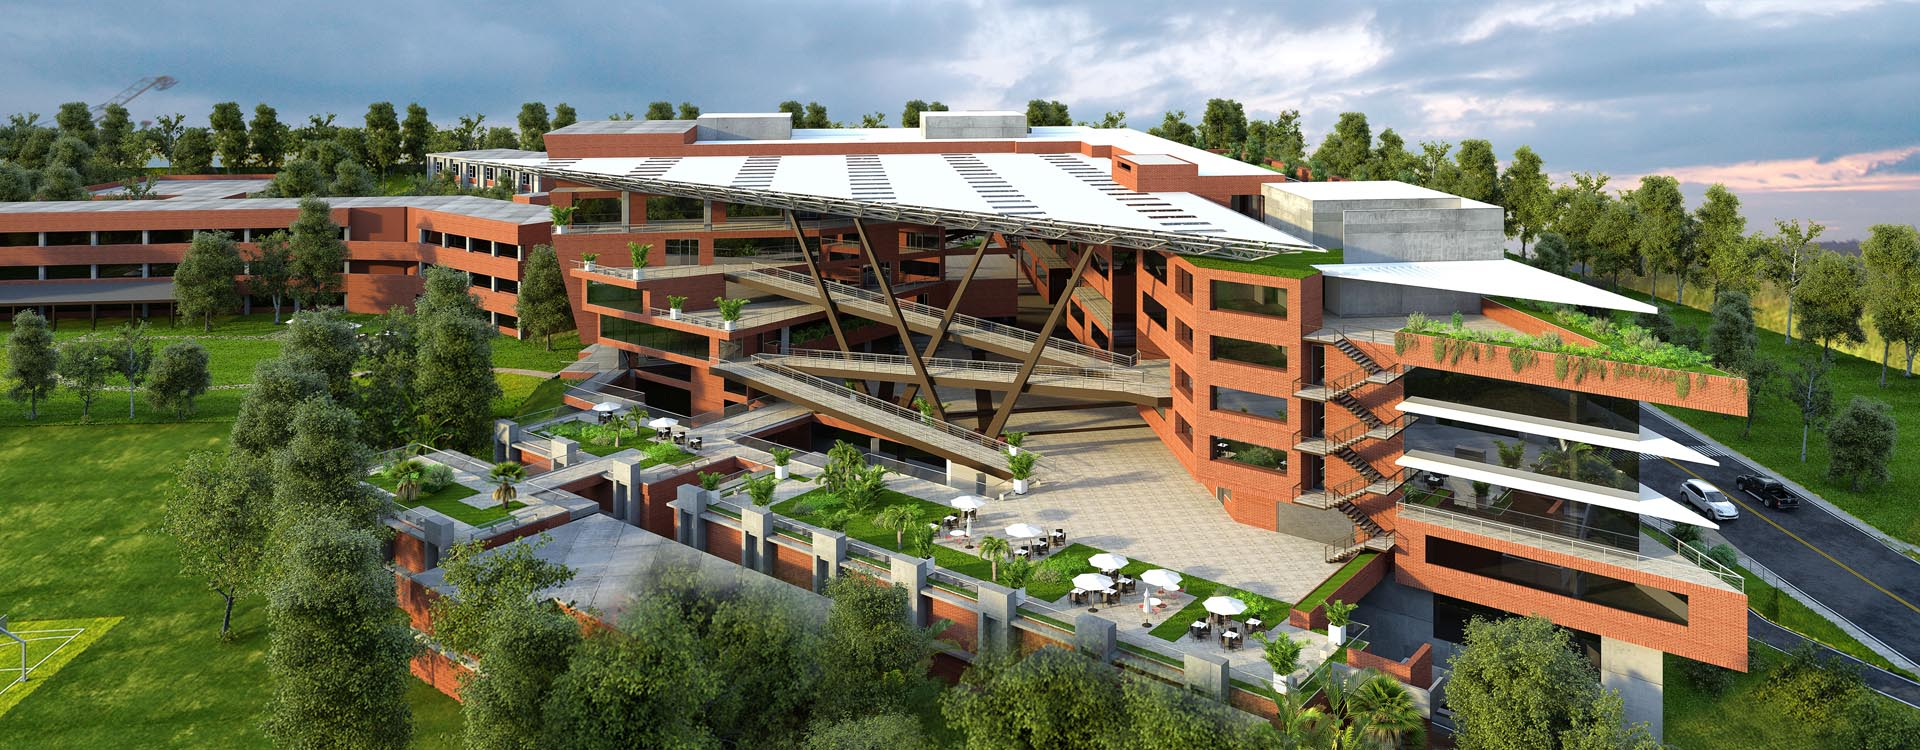
\includegraphics[height=13.25cm]{plantilla/portadacit.jpg}
	\end{figure}
	\restoregeometry
\fi

% ==============================================================================
% PRIMERAS PÁGINAS (Carátulas más hojas de guarda)
% ==============================================================================
\ifdefined\CAPcaratula
	\newpage
    \cleardoublepage\phantomsection
    % \pdfbookmark{Carátula}{toc}
	\pagecolor{white}
	\color{black}
	\setcounter{page}{1}
	\pagenumbering{roman}
	\thispagestyle{empty}
	\begin{center}
		\LARGE UNIVERSIDAD DEL VALLE DE GUATEMALA\\
		\LARGE Facultad de \uvgfacultad \\[0.75cm]
	\end{center}
	\begin{figure}[h]
		\begin{center}
		
\includegraphics[height=5.5 cm]{plantilla/escudoUVGnegro.eps}
		\vspace{0.5in}
		\end{center}
	\end{figure}
	\begin{center}
		\Large \textbf{\nohyphens{\titulotesis}} \\
		%\LARGE \textbf{\titulotesis} \\
		\vfill
		\Large \nohyphens{Trabajo de graduación presentado por \nombreestudiante \ para optar al grado académico de Licenciado en \uvgcarrera} \\
		\vfill
		\large Guatemala, \\
		\vspace{1em}
		\anoentrega
	\end{center}
    
    \ifdefined\printver	
	    \blankpage
	    \blankpage
	    
	    \newpage
	    \cleardoublepage\phantomsection
	    \pagecolor{white}
    	\color{black}
    	\setcounter{page}{1}
    	\pagenumbering{roman}
    	\thispagestyle{empty}
    	\begin{center}
    		\LARGE UNIVERSIDAD DEL VALLE DE GUATEMALA\\
    		\LARGE Facultad de \uvgfacultad \\[0.75cm]
    	\end{center}
    	\begin{figure}[h]
    		\begin{center}
    		
\includegraphics[height=5.5 cm]{plantilla/escudoUVGnegro.eps}
    		\vspace{0.5in}
    		\end{center}
    	\end{figure}
    	\begin{center}
    		\Large \textbf{\nohyphens{\titulotesis}} \\
    		%\LARGE \textbf{\titulotesis} \\
    		\vfill
    		\Large \nohyphens{Trabajo de graduación presentado por \nombreestudiante \ para optar al grado académico de Licenciado en \uvgcarrera} \\
    		\vfill
    		\large Guatemala, \\
    		\vspace{1em}
    		\anoentrega
    	\end{center}
    \fi
\fi

% ==============================================================================
% HOJA DE FIRMAS
% ==============================================================================
\ifdefined\CAPfirmas
	\newpage
	\cleardoublepage\phantomsection
	\thispagestyle{empty}
	\vspace*{0.5in}
	\large Vo.Bo.:\\[1cm]
	\begin{center}
		(f) \rule[1pt]{4 in}{1pt}\\
		\nombreasesor
	\end{center}
	\vspace{1in}

	Tribunal Examinador:\\[1cm]
	\begin{center}
		(f) \rule[1pt]{4 in}{1pt}\\
		\nombreasesor \\[1in]
		(f) \rule[1pt]{4 in}{1pt}\\
		\nombreprimerex \\[1in]
		(f) \rule[1pt]{4 in}{1pt}\\
		\nombresegundoex
	\end{center}
	\vspace{1in}

%	Fecha de aprobación: Guatemala, \rule[1pt]{0.5 in}{1pt} de \rule[1pt]{1 in}{1pt} de \anoaprobacion.
    Fecha de aprobación: Guatemala, \diaaprobacion de \mesaprobacion de \anoaprobacion.
	\normalsize
\fi

% Comentar para formato estilo libro en la numeración de páginas (NO 
% compatible con la guía UVG 2019)
\pagestyle{plain}
% ==============================================================================
% CONTENIDO DEL TRABAJO
% ==============================================================================
% PREFACIO
% ------------------------------------------------------------------------------
\ifdefined\CAPprefacio
	\newpage
	\cleardoublepage\phantomsection
    \chapter*{Prefacio}
    \ifdefined\parpordefecto
    	\defaultparformat{a-prefacio}
    \else
    	Lorem ipsum dolor sit amet, consectetur adipiscing elit. Cras vitae eleifend ipsum, ut mattis nunc. Pellentesque ac hendrerit lacus. Cras sollicitudin eget sem nec luctus. Vivamus aliquet lorem id elit venenatis pellentesque. Nam id orci iaculis, rutrum ipsum vel, porttitor magna. Etiam molestie vel elit sed suscipit. Proin dui risus, scelerisque porttitor cursus ac, tempor eget turpis. Aliquam ultricies congue ligula ac ornare. Duis id purus eu ex pharetra feugiat. Vivamus ac orci arcu. Nulla id diam quis erat rhoncus hendrerit. Class aptent taciti sociosqu ad litora torquent per conubia nostra, per inceptos himenaeos. Sed vulputate, metus vel efficitur fringilla, orci ex ultricies augue, sit amet rhoncus ex purus ut massa. Nam pharetra ipsum consequat est blandit, sed commodo nunc scelerisque. Maecenas ut suscipit libero. Sed vel euismod tellus.

Proin elit tellus, finibus et metus et, vestibulum ullamcorper est. Nulla viverra nisl id libero sodales, a porttitor est congue. Maecenas semper, felis ut rhoncus cursus, leo magna convallis ligula, at vehicula neque quam at ipsum. Integer commodo mattis eros sit amet tristique. Cras eu maximus arcu. Morbi condimentum dignissim enim non hendrerit. Sed molestie erat sit amet porttitor sagittis. Maecenas porttitor tincidunt erat, ac lacinia lacus sodales faucibus. Integer nec laoreet massa. Proin a arcu lorem. Donec at tincidunt arcu, et sodales neque. Morbi rhoncus, ligula porta lobortis faucibus, magna diam aliquet felis, nec ultrices metus turpis et libero. Integer efficitur erat dolor, quis iaculis metus dignissim eu.
    \fi
    \addcontentsline{toc}{chapter}{Prefacio}
\fi

% ÍNDICE GENERAL
% ------------------------------------------------------------------------------
\ifdefined\CAPindice
	\newpage
    \cleardoublepage\phantomsection
	\renewcommand{\contentsname}{Índice}
    %\phantomsection
    \pdfbookmark{\contentsname}{toc}
    %\pdfbookmark{Índice}{toc}
	\tableofcontents
\fi

% LISTADO DE FIGURAS
% ------------------------------------------------------------------------------
\ifdefined\CAPfiguras
	\newpage
    \cleardoublepage\phantomsection
	\renewcommand{\listfigurename}{Lista de figuras}
	\listoffigures
	\addcontentsline{toc}{chapter}{Lista de figuras}
\fi

% LISTADO DE CUADROS
% ------------------------------------------------------------------------------
\ifdefined\CAPcuadros
	\newpage
    \cleardoublepage\phantomsection
	\renewcommand{\listtablename}{Lista de cuadros}
	\listoftables
	\addcontentsline{toc}{chapter}{Lista de cuadros}
\fi

% RESUMEN
% ------------------------------------------------------------------------------
\ifdefined\CAPresumen
	\newpage
    \cleardoublepage\phantomsection
	\chapter*{Resumen}
	\ifdefined\parpordefecto
		\defaultparformat{b-resumen}
	\else
		Lorem ipsum dolor sit amet, consectetur adipiscing elit. Cras vitae eleifend ipsum, ut mattis nunc. Pellentesque ac hendrerit lacus. Cras sollicitudin eget sem nec luctus. Vivamus aliquet lorem id elit venenatis pellentesque. Nam id orci iaculis, rutrum ipsum vel, porttitor magna. Etiam molestie vel elit sed suscipit. Proin dui risus, scelerisque porttitor cursus ac, tempor eget turpis. Aliquam ultricies congue ligula ac ornare. Duis id purus eu ex pharetra feugiat. Vivamus ac orci arcu. Nulla id diam quis erat rhoncus hendrerit. Class aptent taciti sociosqu ad litora torquent per conubia nostra, per inceptos himenaeos. Sed vulputate, metus vel efficitur fringilla, orci ex ultricies augue, sit amet rhoncus ex purus ut massa. Nam pharetra ipsum consequat est blandit, sed commodo nunc scelerisque. Maecenas ut suscipit libero. Sed vel euismod tellus.

Proin elit tellus, finibus et metus et, vestibulum ullamcorper est. Nulla viverra nisl id libero sodales, a porttitor est congue. Maecenas semper, felis ut rhoncus cursus, leo magna convallis ligula, at vehicula neque quam at ipsum. Integer commodo mattis eros sit amet tristique. Cras eu maximus arcu. Morbi condimentum dignissim enim non hendrerit. Sed molestie erat sit amet porttitor sagittis. Maecenas porttitor tincidunt erat, ac lacinia lacus sodales faucibus. Integer nec laoreet massa. Proin a arcu lorem. Donec at tincidunt arcu, et sodales neque. Morbi rhoncus, ligula porta lobortis faucibus, magna diam aliquet felis, nec ultrices metus turpis et libero. Integer efficitur erat dolor, quis iaculis metus dignissim eu.
	\fi
	\addcontentsline{toc}{chapter}{Resumen}
\fi

% ABSTRACT
% ------------------------------------------------------------------------------
\ifdefined\CAPabstract
	\newpage
    \cleardoublepage\phantomsection
	\chapter*{Abstract}
	\ifdefined\parpordefecto
		\defaultparformat{c-abstract}
	\else
		In this graduation work, the implementation of the swarm intelligence algorithm focused on synchronization and control of robotic system formations was optimized. For its development, Pololu 3Pi+ differential robots were used within the Robotat ecosystem of the Universidad del Valle de Guatemala.

The process began by verifying the performance of the original algorithm, using simulations with Webots and in physical scenarios. Then, areas of improvement in its implementation were identified, focusing on increasing scalability, robustness and computational efficiency through the use of matrix operations, parallelism, adjustments in position allocation and improving other functionalities.

As part of the validation, $24$ experiments were carried out to verity the performance of the optimized algorithm. The results showed a significant reduction in execution times, particularly as the number of agents in the formation increased. As an example, in experiments with $5$ agents the average time was $143.224$ seconds with the optimized version, compared to $335.378$ seconds for the original version, using scenarios with equal conditions.

Finally, the optimized algorithm was shown to be suitable for generating trajectories in scenarios with moving obstacles. This was validated with $26$ controlled physical experiments, in which agents adjusted their trajectories in real time, responded to changes in obstacle positions and avoided collisions, confirming the effectiveness and adaptability of the algorithm.
	\fi
	\addcontentsline{toc}{chapter}{Abstract}
\fi

% INTRODUCCIÓN
% ------------------------------------------------------------------------------
\ifdefined\CAPintroduccion
	\newpage
	\cleardoublepage
	\pagenumbering{arabic}
	\setcounter{page}{1}
	\chapter{Introducción}
	\ifdefined\parpordefecto
		\defaultparformat{d-introduccion}
	\else
		El objetivo de este proyecto fue continuar indagando en la robótica de enjambre al seguir con el desarrollo e implementación de un algoritmo de sincronización y control de formaciones de sistemas robóticos multi-agente. Durante las fases previas se llegó hasta la validación del algoritmo en un entorno real utilizando el ecosistema del Robotat de la Universidad del Valle de Guatemala (UVG), sin embargo, no se profundizó en su funcionamiento al utilizar escenarios con obstáculos móviles. A pesar de esto, se dejó una buena infraestructura en cuando a código y su implementación en el Robotat para seguir explorando el alcance del algoritmo con escenarios más complejos.

El propósito de este proyecto fue optimizar la implementación del algoritmo de inteligencia de enjambre desarrollado anteriormente, y validarlo en escenarios con obstáculos móviles en el ecosistema del Robotat. Para cumplir con esto, se utilizó el sistema de captura de movimiento OptiTrack, la mesa de pruebas, los agentes robóticos Pololu 3Pi+ modificados y red de comunicación con el servidor del Robotat.

En primer lugar, se llevó a cabo el levantamiento de la fase preliminar del algoritmo, para lo cual se simularon escenarios en WebotsR2023b. Una vez que las simulaciones funcionaron correctamente, se buscó replicar el funcionamiento del algoritmo en el Robotat. Durante este proceso, se encontró con obstáculos como que se realizaron cambios en las conexiones de los Pololu 3Pi+, modificaciones en los marcadores disponibles y la necesidad de ajustar los parámetros de control. Todo este proceso se describe a detalle en el Capítulo \ref{cap:restauracion}.

Una vez replicado el funcionamiento del algoritmo en simulación y físico, se puso a prueba su naturaleza dinámica. En el Capítulo \ref{cap:naturaleta_dinamica} se explica a detalle cómo funciona y se muestran los escenarios de prueba utilizados.

El siguiente paso fue optimizar la implementación del algoritmo. Para esto, se identificaron deficiencias y puntos de mejora en el código, lenguaje de programación y métodos de comunicación. En el Capítulo \ref{cap:optimizacion} se detalla el proceso realizado y en el Capítulo \ref{cap:verificacion_optim} se muestran los resultados de la optimización.

Finalmente, en el Capítulo \ref{cap:validacion} se muestra la validación del algoritmo optimizado utilizando escenarios con obstáculos móviles en el Robotat.
	\fi
\fi

% ANTECEDENTES
% ------------------------------------------------------------------------------
\ifdefined\CAPantecedentes
	\newpage
	\chapter{Antecedentes}
	\ifdefined\parpordefecto
    	\defaultparformat{e-antecedentes}
    \else
    	\section{Robótica de enjambre}
La robótica de enjambre consiste en el uso de robots relativamente sencillos que, al organizarse y funcionar en conjunto, pueden llevar a cabo tareas complejas que un solo robot no podría realizar \cite{robotica_enjambre2}. Esto proporciona soluciones flexibles, optimizadas y de un menor costo. Además, no se requiere un número específico de agentes robóticos ya que pueden ir desde las dos unidades hasta miles de ellas \cite{UNIDIRswarm}.

Algunas de las aplicaciones de la robótica de enjambre son el control de tráfico, realizar formaciones en movimiento, misiones de búsqueda y rescate, mapeo de entornos, simulación de comportamientos biológicos, exploración de zonas y comunicación de rutas. 

Estas últimas dos han sido estudiadas a profundidad para su implementación en la cosecha de la fresa donde el enjambre realiza la exploración de una zona de cultivo, analiza el estado de los frutos por medio de imágenes computacionales para determinar el momento óptimo para su cosecha y comunica los datos procesados para realizar una cosecha automatizada \cite{EnjambresCultivos}.

\subsection{Robótica de enjambre inspirada en peces}
En 2021 un equipo de investigadores del instituto Wyss de Harvard y la Escuela de Ingeniería y Ciencias Aplicadas John A. Paulson (SEAS) desarrollaron un robot llamado Bluebot inspirado en un pez. Este cuenta con dos cámaras y tres luces LED para su sistema de visión guiado. 

Los investigadores simularon una misión de búsqueda con una luz roja intermitente e implementaron un algoritmo de dispersión. Para iniciar, los Bluebots se dispersaron en el tanque y una vez que un robot detectó la luz roja, sus leds comenzaron a parpadear, lo que activó el algoritmo de agregación al resto de robots que lograron sincronizar sus movimientos y agruparse al rededor del robot que detectó la luz, imitando a un banco de peces real \cite{Bluebot}.

\begin{figure}[H]
	\centering
	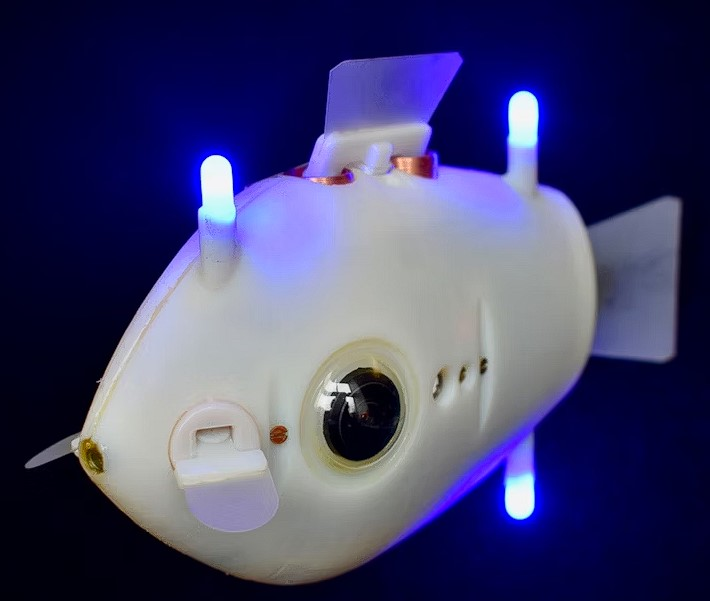
\includegraphics[width=0.5\textwidth]{Bluebot.jpg}
	\caption{Prototipo físico de Bluebot\cite{Bluebot}.}
	\label{fig:bluebot}
\end{figure}

\section{Robotarium de Georgia Tech}
En el Instituto Tecnológico de Georgia se ha desarrollado el proyecto Robotarium \cite{Robotarium}. Se realizó para proveer acceso gratuito a una plataforma de robótica de enjambre a la que pueda acceder cualquier persona del mundo. Lo único que se necesita para experimentar con la plataforma es descargar un simulador en Matlab o Python, registrarse en la página de Robotarium y esperar la aprobación por parte de un administrador para realizar el experimento.

\begin{figure}[H]
	\centering
	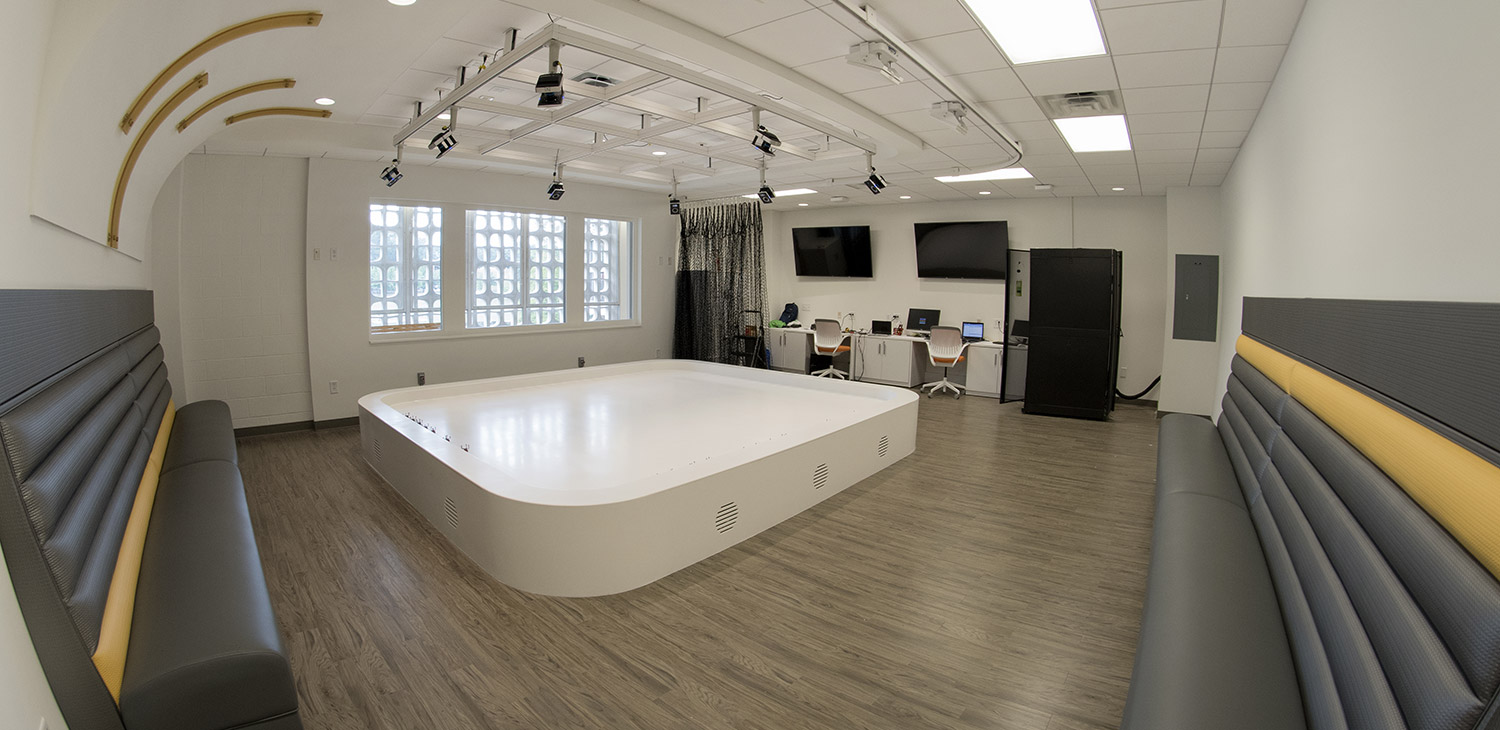
\includegraphics[width=0.5\textwidth]{robotarium.jpg}
	\caption{Laboratorio Robotarium de Georgia Tech \cite{Robotarium}.}
	\label{fig:robotarium}
\end{figure}

\section{Robotat de la Universidad del Valle de Guatemala}
En el Centro de Innovación y Tecnología de la Universidad del Valle de Guatemala, se encuentra una plataforma de robótica para experimentación llamada Robotat la cual está inspirada en el Robotarium del Instituto Tecnológico de Georgia. Esta se conforma de una plataforma de acero y plycem con un espacio útil de 5 $\times$ 5 $\times$ 3 m, capaz de soportar cargas puntuales de hasta dos toneladas. También cuenta con un sistema de captura de movimiento de OptiTrack, compuesto de seis cámaras Prime$^x$ 41 de alta precisión y baja latencia para realizar experimentos en tiempo real. Además, el sistema funciona con una red local inalámbrica WiFi a través de la cual se realiza la comunicación entre robots \cite{Robotat}. 

Para el funcionamiento del sistema OptiTrack, se utilizan ``marcadores'' que son figuras plásticas con reflectivos. Estos permiten reflejar la luz infrarroja que emiten las cámaras para obtener, de manera precisa, la posición y el movimiento de objetos en un espacio tridimensional.

\begin{figure}[H]
	\centering
	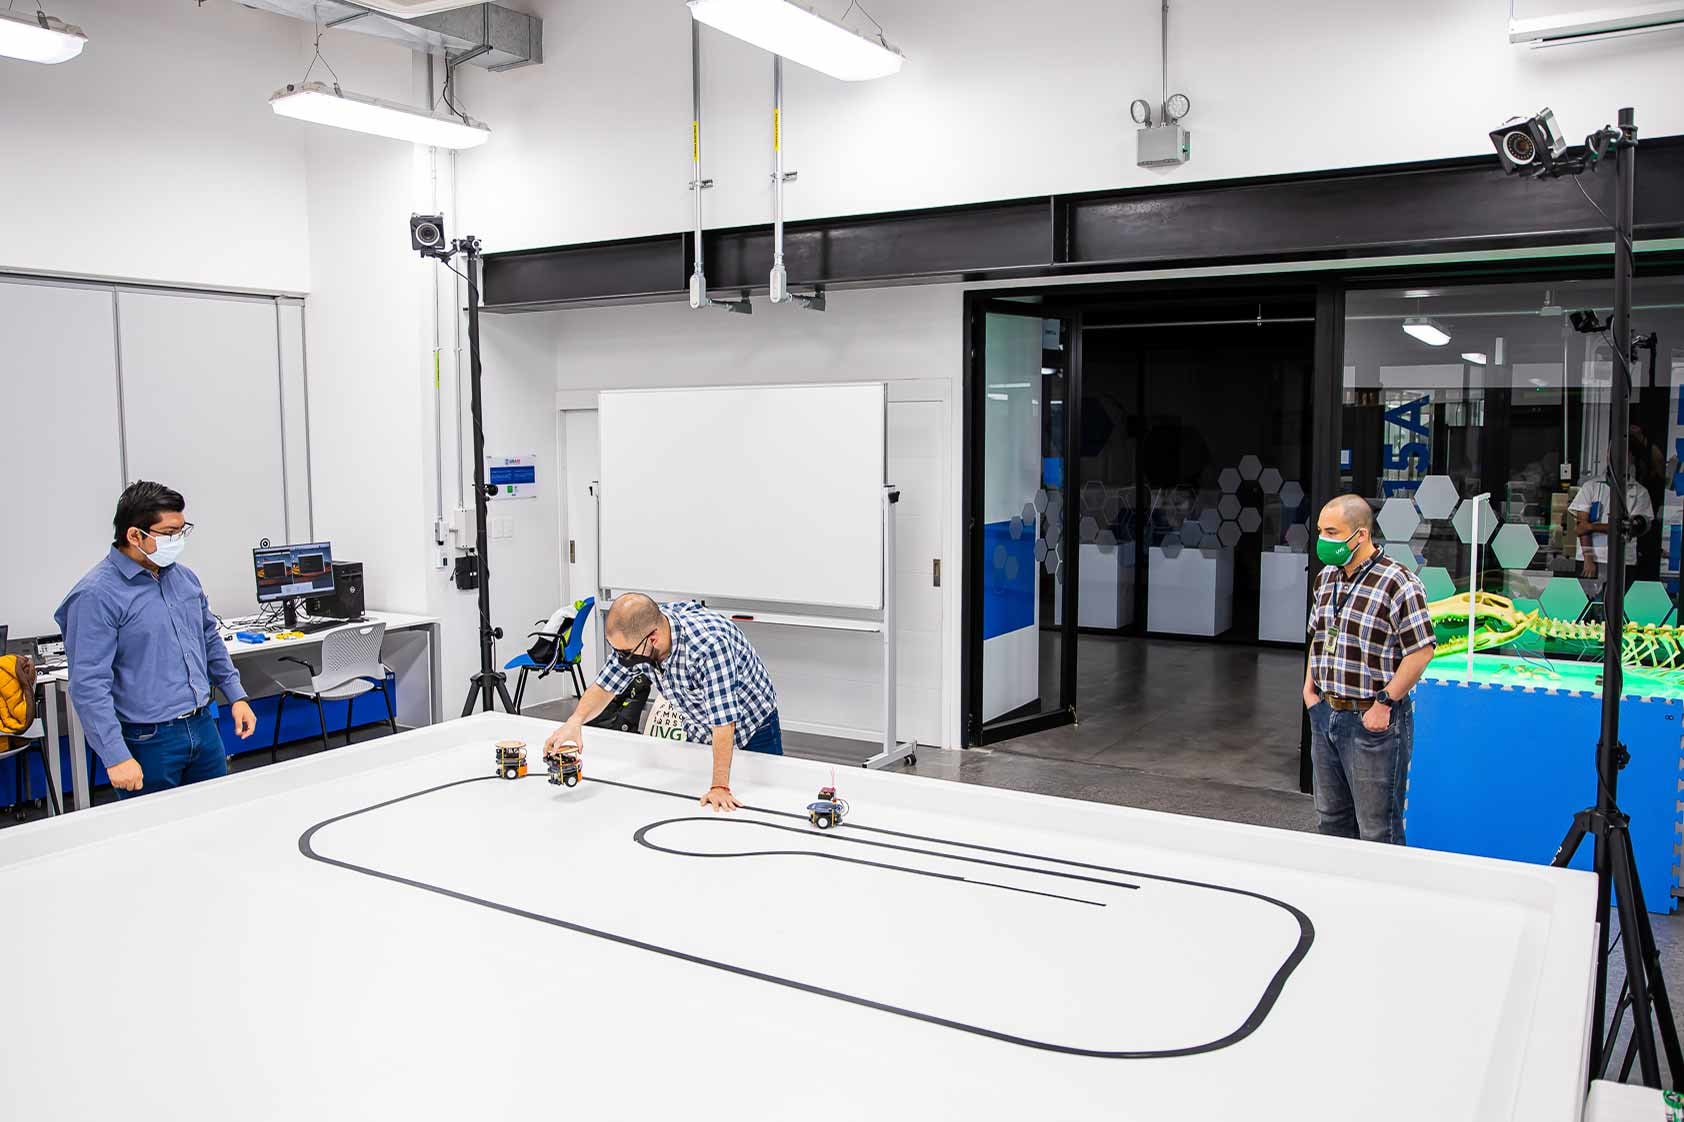
\includegraphics[width=0.5\textwidth]{robotatUVG.jpg}
	\caption{Plataforma Robotat de la Universidad del Valle de Guatemala \cite{imgRobotat}.}
	\label{fig:robotat}
\end{figure}

\section{Trabajos previos de robótica de enjambre en la UVG}
A continuación se presentan algunos de los trabajos realizados en el área de robótica de enjambre.

\subsection{Validación de algoritmos de algoritmos de \textit{Particle Swarm Optimization} (PSO) y \textit{Ant Colony Optimization} (ACO)}
La tesis de Jonathan Menéndez \cite{MenendezJ_2023_tesis} se enfocó en realizar pruebas físicas para validar los algoritmos de robótica de enjambre PSO y ACO utilizando los robots móviles Pololu 3pi+ en la plataforma de Robotat. 

Luego de realizar múltiples pruebas físicas, se encontró que el algoritmo de ACO es capaz de generar trayectorias de manera satisfactoria en el ecosistema del Robotat, respetando las limitaciones físicas de espacio en la mesa para no colisionar y evitar que las cámaras de OptiTrack pierdan la detección de los agentes. Además, este algoritmo demostró tener una mayor eficiencia al corregir las diferencias entre el nodo de inicio y la posición inicial del robot al orientarlo hacia el punto de inicio. 

Dichos estudios se limitaron al espacio disponible en la mesa de la plataforma del Robotat, a un espacio libre de obstáculos y a la implementación de solo diez Pololu 3pi+ debido a la disponibilidad de equipo. 

\subsection{Algoritmo de sincronización y control de sistemas de robots multiagente para misiones de búsqueda}
El trabajo de investigación de Andrea Maybell Peña \cite{PenaAM_2019_tesis} se basó en utilizar un sistema de robots multi-agente para realizar misiones de búsqueda. El algoritmo se basa en la teoría de grafos y el control moderno para tener formaciones específicas de los agentes que permiten su movilización a través de obstáculos que se limitaron a una geometría toroidal y la cantidad de agentes robóticos se limitó a diez unidades del modelo E-Puck de GCtronic.

Se realizó la implementación del algoritmo en el simulador Webots de Cyberbotics. Como resultado se obtuvo una tasa de éxito del 80\% utilizando el algoritmo completo para llegar a la meta.

\begin{figure}[H]
	\centering
	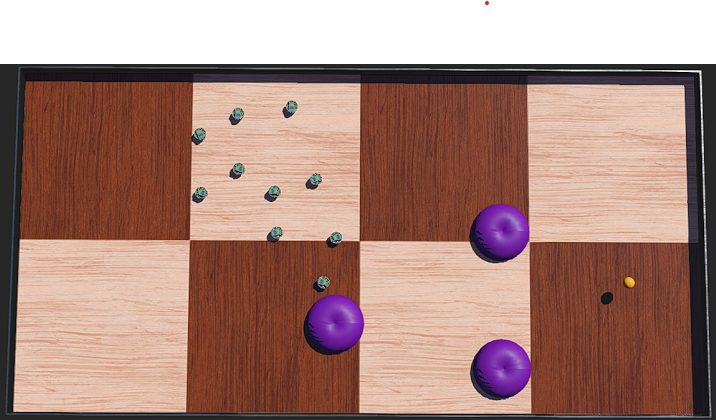
\includegraphics[width=0.4\textwidth]{simulacion_inicio_tesis_andreaPena.png} 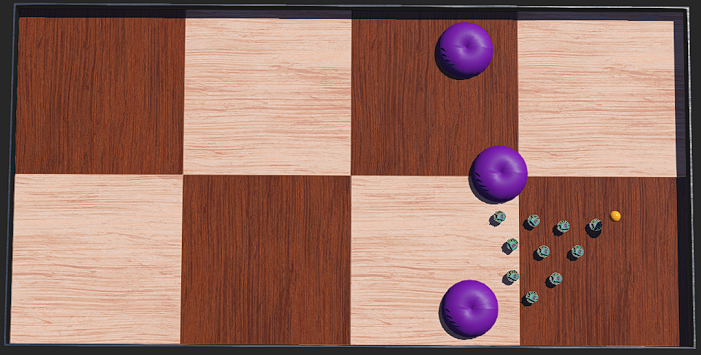
\includegraphics[width=0.4\textwidth]{simulacion_final_tesis_andreaPena.png}
	\caption{Simulación en Webots implementando el algoritmo para evadir obstáculos \cite{imgRobotat}.}
	\label{fig:tesis_andreaPena}
\end{figure}

\subsection{Validación de un algoritmo de inteligencia de enjambre enfocado en sincronización y control de formaciones de sistemas robóticos multi-agente en un entorno físico}
En el trabajo de investigación de Alejandro Rodríguez \cite{RodriguezJA_2023_tesis}se realizó una validación del algoritmo de inteligencia de enjambre enfocado a sincronización vertical y control de formaciones de sistemas robóticos multi-agente. La validación se realizó utilizando el ecosistema del Robotat de la Universidad del Valle de Guatemala y los robots Pololu 3pi+ modificados.

Para la validación física, se realizaron diversos experimentos donde se evaluó el desempeño de cada agente, la generación de trayectorias, el posicionamiento de los agentes, las distintas configuraciones de formación y los escenarios utilizando obstáculos.

Los experimentos realizados se limitaron a utilizar un máximo de nueve agentes robóticos debido a su disponibilidad en la universidad, el tiempo máximo por semana para realizar pruebas en el Robotat fue de seis horas y estas se realizaron utilizando obstáculos estáticos.

Los resultados de la experimentación demostraron que, el algoritmo evade los obstáculos satisfactoriamente y mantiene una distancia adecuada entre agentes. Sin embargo, el algoritmo en simulación es aproximadamente un 70\% más rápido que en físico. Esto se debe a que cada prueba física tomaba al rededor de 8 minutos debido a la latencia del servidor que aumentaba con el número de agentes conectados. 



    \fi  
\fi

% JUSTIFICACIÓN
% ------------------------------------------------------------------------------
\ifdefined\CAPjustificacion
	\newpage
	\chapter{Justificación}
	\ifdefined\parpordefecto
		\defaultparformat{f-justificacion}
	\else
		La inteligencia de enjambre es un campo reciente en el área de inteligencia artificial. Sus aplicaciones abarcan desde realizar tareas cotidianas hasta resolver problemas complejos. Uno de sus mayores beneficios es utilizar agentes robóticos de bajo costo para ejecutar acciones en conjunto en lugar de utilizar un solo robot complejo. Además, esto crea un sistema robótico robusto lo que resulta útil para diversas aplicaciones.

Se decidió estudiar la robótica de enjambre ya que en la Universidad del Valle de Guatemala, en trabajos anteriores, se han realizado pruebas implementando algoritmos de sincronización y control utilizando simuladores como Webots, así como agentes físicos Pololu 3Pi+. Estas pruebas tuvieron éxito, sin embargo, estuvieron limitadas a generar trayectorias en un ambiente con obstáculos fijos y los tiempos de ejecución eran muy largos. Por lo tanto, en este trabajo de graduación se desea optimizar el algoritmo desarrollado previamente y realizar nuevas pruebas para validar las trayectorias generadas en un ambiente controlado con obstáculos móviles. 

Esto permitirá conocer el alcance de los algoritmos de sincronización y control, además que abrirá las puertas a su implementación en aplicaciones de la vida real como misiones de búsqueda y rescate o análisis de zonas de cultivos, donde en los escenarios se encontrarán obstáculos móviles como personas, animales o incluso cambios en el propio escenario debido a factores externos.

	\fi
\fi

% OBJETIVOS
% ------------------------------------------------------------------------------
\ifdefined\CAPobjetivos
	\newpage
	\chapter{Objetivos}
	\ifdefined\parpordefecto
		\defaultparformat{g-objetivos}
	\else
		\section{Objetivo general}
Optimizar la implementación del algoritmo de inteligencia de enjambre enfocado en sincronización y control de formaciones de sistemas robóticos multi-agente desarrollado anteriormente, y validarlo en escenarios con obstáculos móviles, en el ecosistema Robotat.

\section{Objetivos específicos}
\begin{itemize}
	\item Evaluar la implementación del algoritmo de sincronización y control desarrollado anteriormente e identificar deficiencias y puntos de mejora en código, lenguaje de programación y métodos de comunicación.

	\item Optimizar el algoritmo tomando en cuenta los puntos de mejora identificados y evaluar su rendimiento en escenarios similares a los utilizados anteriormente.
	
	\item Adaptar el algoritmo para generar trayectorias en escenarios con obstáculos móviles.
	
	\item Validar el rendimiento del algoritmo optimizado con agentes robóticos como el Pololu 3Pi+ en el ecosistema Robotat.
\end{itemize}
	\fi
\fi

% ALCANCE
% ------------------------------------------------------------------------------
\ifdefined\CAPalcance
	\newpage
	\chapter{Alcance}
	\ifdefined\parpordefecto
    	\defaultparformat{h-alcance}
    \else
    	Podemos usar \Gls{latex} para escribir de forma ordenada una \gls{formula} matemática. 
    \fi 
\fi

% MARCO TEÓRICO
% ------------------------------------------------------------------------------
\ifdefined\CAPmarcoteorico
	\newpage
	\chapter{Marco teórico}
	\ifdefined\parpordefecto
		\defaultparformat{i-marco_teorico}
	\else
		\section{Conceptos fundamentales en robótica de enjambre}

\subsection{Enjambre}
En la robótica, un enjambre es el conjunto de individuos que colaboran entre sí para lograr un objetivo \cite{robotica_enjambre3}. En la Figura \ref{fig:enjambre} se muestra un enjambre de robots.

\begin{figure}[H]
	\centering
	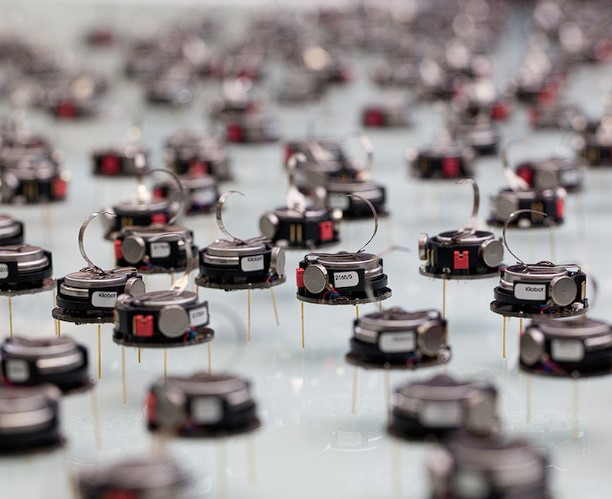
\includegraphics[width=0.6\textwidth]{enjambre.jpg}
	\caption{Ejemplo de enjambre de robots \cite{imgEnjambre}.}
	\label{fig:enjambre}
\end{figure}

\subsection{Agente}
Se le conoce como agente a un individuo que forma parte del enjambre. Este es capaz de realizar acciones simples para lograr un objetivo de forma colaborativa con los demás individuos. En la robótica de enjambre, los agentes son robots \cite{definiciones_robotica_enjambre}.

\subsection{Formaciones}
Es común que en la naturaleza se observen enjambres que forman patrones. Esto es gracias a que los individuos realizan movimientos coordinados para crear formaciones. En la robótica de enjambre sucede lo mismo, se tiene un conjunto de agentes que se organizan y coordinan sus movimientos para lograr objetivos. Estos pueden ser evadir obstáculos, mapear un entorno, llegar a un objetivo siguiendo una trayectoria, entre otros. Para lograr la coordinación de formaciones, se requiere aplicar un control que puede ser centralizado o descentralizado \cite{definiciones_robotica_enjambre}.

\subsection{Control centralizado y descentralizado}
En la robótica de enjambre, el control centralizado consiste en una red de comunicación donde una unidad central de procesamiento (CPU) tiene comunicación con cada agente para transmitir y recibir información. Asimismo, cada agente se comunica únicamente con el CPU.

El control descentralizado, también llamado control distribuido, es donde cada agente tiene comunicación con los demás para transmitir información. Este tipo de control requiere un protocolo de comunicación más robusto y complejo, sin necesidad de un CPU \cite{Control_centralizado_descentralizado}.

En la Figura \ref{fig:control_centralizado_descentralizado} se observa la diferencia entre ambos tipos de control.

\begin{figure}[H]
	\centering
	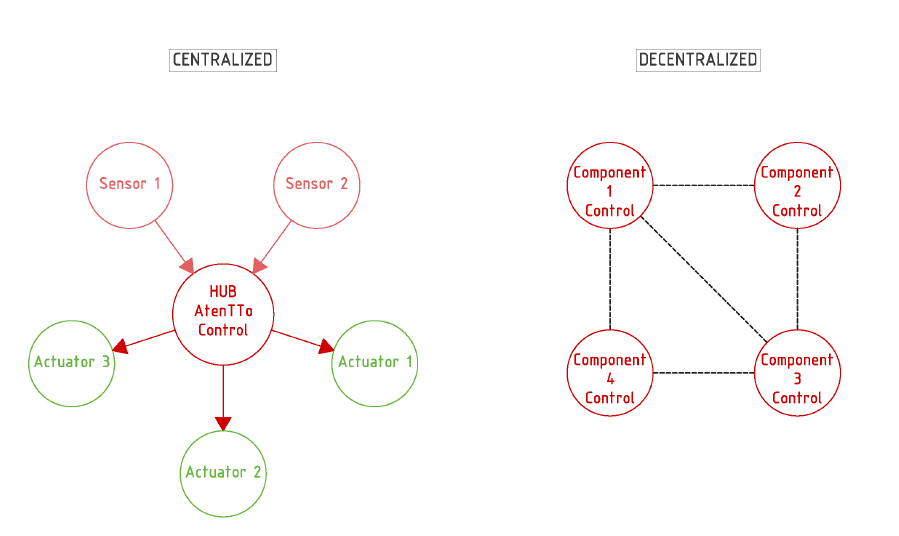
\includegraphics[width=1\textwidth]{control_centralizado_descentralizado.png}
	\caption{Ejemplo de un control centralizado y descentralizado \cite{Control_centralizado_descentralizado}.}
	\label{fig:control_centralizado_descentralizado}
\end{figure}


\section{Conceptos básicos en teoría de grafos}

\subsection{Teoría de grafos}
La teoría de grafos es una rama de la matemática y ciencias de la computación que se dedica a estudiar los grafos \cite{teoria_de_grafos}. El grafo es un conjunto de vértices conectados por aristas tal como se observa en la Figura \ref{fig:teoria_de_grafos}. Esta teoría se utiliza en diversas aplicaciones como mapeo de entornos, generación de rutas, análisis de datos, telecomunicaciones, entre otras. En este trabajo de graduación, se utilizó la teoría de grafos para definir formaciones y la red de comunicación entre agentes.

\begin{figure}[H]
	\centering
	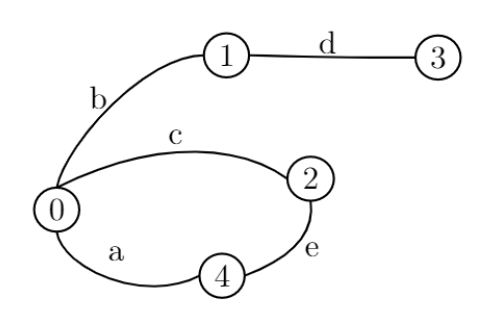
\includegraphics[width=0.5\textwidth]{grafo_matrices_andrea.png}
	\caption{Ejemplo de un grafo \cite{PenaAM_2019_tesis}.}
	\label{fig:teoria_de_grafos}
\end{figure}

\subsection{Vértices y aristas}
Los vértices, también llamados nodos, son los puntos donde se conectan las aristas de un grafo. El grado de un vértice será el número de aristas asociados a él \cite{teoria_de_grafos}. 

Las aristas, también llamadas arcos o enlaces, son las líneas que conectan un par de vértices y se clasifican en \cite{teoria_de_grafos}:

\begin{itemize}
	\item Lazo: Es una arista que tiene en sus extremos el mismo vértice. 
	\item Paralelas o múltiples: Es cuando dos o más aristas tienen en los extremos el mismo par de vértices.
\end{itemize}

\subsection{Tipos de grafos}
En un grafo, los vértices se puede conectar de distintas maneras según la aplicación que se requiera tal como se observa en la Figura \ref{fig:tipos_de_grafos}. Algunas de sus clasificaciones son \cite{tipos_de_grafos}:

\begin{itemize}
	\item Simple o anillo: Cada par de nodos se conecta por una sola arista.
	\item Multigrafo: En cada par de nodos puede haber más de un enlace.
	\item Árbol: Es un grafo que no tiene ciclos.
	\item Dirigidos o dígrafos: Las aristas entre los nodos tienen dirección.
	\item Estrella: Tiene un nodo central que conecta con los demás nodos.
	\item No conexos: Hay uno o más nodos que no conectan con el resto.
	\item Completo: Cada nodo está conectado con los demás.
	\item Regular: Todos los nodos tienen el mismo número de aristas.
	\item De celosía y mundo pequeño: Estos grafos se utilizan para entender el comportamiento y estructura de ciertos fenómenos en la naturaleza.
\end{itemize}

\begin{figure}[H]
	\centering
	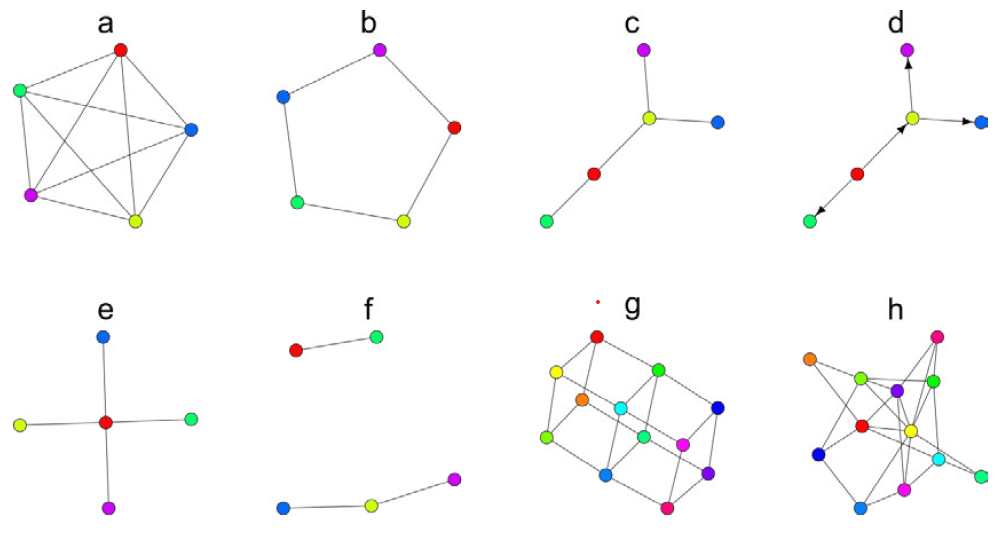
\includegraphics[width=1\textwidth]{tipos_de_grafos.png}
	\caption{Ejemplo de algunos tipos de grafos. a: completo, b: simple, c: árbol, d: dígrafo, e: estrella, f: no conexo, g: de celosía, h: de mundo pequeño \cite{tipos_de_grafos}.}
	\label{fig:tipos_de_grafos}
\end{figure}

\subsection{Matrices asociadas a un grafo}
La representación gráfica de un grafo es poco práctica para su análisis, por esto es mejor utilizar su representación matricial \cite{FrancoF_2016_trabajo_fin_de_grado}. A continuación, se mencionan algunas matrices útiles y su implementación para el grafo de la Figura \ref{fig:teoria_de_grafos}.


\begin{itemize}
	\item Matriz de incidencia (I): Se tiene una matriz de $v$ vértices por $e$ aristas. El elemento $a_{ve} = 1 $ si la arista conecta con el vértice, de lo contrario $a_{ve} = 0$.
	
	\[
	I = 
	\left[\begin{array}{ccccc}
		1 & 1 & 1 & 0 & 0 \\
		0 & 1 & 0 & 1 & 0 \\
		0 & 0 & 1 & 0 & 1 \\
		0 & 0 & 0 & 1 & 0 \\
		1 & 0 & 0 & 0 & 1 \\
	\end{array} \right]
	\]
	
	\item Matriz de adyacencia (A): El grafo se representa con una matriz cuadrada de tamaño $v \times v$. Si hay una arista entre el vértice $v_1$ y $v_2$ , el elemento $a_{v_1 v_2} = 1$.
	
	\[
	A = 
	\left[\begin{array}{ccccc}
		1 & 1 & 0 & 0 & 0 \\
		0 & 0 & 1 & 1 & 0 \\
		0 & 0 & 0 & 1 & 0 \\
		0 & 0 & 0 & 0 & 0 \\
		0 & 0 & 0 & 0 & 0 \\
	\end{array} \right]
	\]
	
	\item Matriz de grados (D): Se tiene una matriz diagonal de tamaño $v \times v$ que contiene los grados de cada vértice. 
	
	\[
	D = 
	\left[\begin{array}{ccccc}
		3 & 0 & 0 & 0 & 0 \\
		0 & 2 & 0 & 0 & 0 \\
		0 & 0 & 2 & 0 & 0 \\
		0 & 0 & 0 & 1 & 0 \\
		0 & 0 & 0 & 0 & 2 \\
	\end{array} \right]
	\]
	
	\item Matriz laplaciana (L): Esta matriz es resultado de operar otras matrices asociadas al grafo. Para grafos no dirigidos, esta se calcula como $L = D - A$. Para grafos dirigidos se calcula como $L = I I^T$.
	
	\[
	l = 
	\left[\begin{array}{ccccc}
		3 & -1 & -1 & 0 & -1 \\
		-1 & 2 & 0 & -1 & 0 \\
		-1 & 0 & 2 & 0 & -1 \\
		0 & -1 & 0 & 1 & 0 \\
		-1 & 0 & -1 & 0 & 2 \\
	\end{array} \right]
	\]
	
	\item Matriz de rigidez (K): Esta matriz surge de qué tanto es posible deformar el grafo sin doblar ni modificar la longitud de las aristas \cite{matrices_asociadas_grafos}. A continuación se muestra la matriz de adyacencia totalmente rígida.
	
	\[
	A = 
	\left[\begin{array}{ccccc}
		1 & 1 & 0 & 0 & 0 \\
		0 & 0 & 1 & 1 & 0 \\
		0 & 0 & 0 & 1 & 0 \\
		0 & 0 & 0 & 0 & 0 \\
		0 & 0 & 0 & 0 & 0 \\
	\end{array} \right]
	\]
	
	Esta corresponde a la matriz de adyacencia del grafo completo.
	
\end{itemize}


\section{Control de la formación}
Para resolver el problema de control de formaciones se utilizan dos grafos asociados. El primero es el grafo de formación. Este es un grafo no dirigido que contiene la configuración deseada. Además, se utiliza un grafo ponderado donde las longitudes de las aristas representan la distancia entre los agentes. El segundo grafo es el que representa la red de comunicación entre agentes. Este es un grafo dirigido donde las aristas están definidas por la dinámica de lazo cerrado del sistema multi-agente \cite{PenaAM_2019_tesis}. 

\subsection{Grafo de formación}
Para definir un grafo de formación se debe entender el concepto de rigidez. Una estructura es rígida cuando todas las distancias entre los vértices están definidas y se mantienen constantes. Para evaluar la rigidez de un grafo se debe cumplir $e = 2v - 3$, donde $v$ es el número de vértices y $e$ el número de aristas. Si un grafo tiene menos aristas que vértices, este ya no se considera rígido \cite{KrickL_2007_tesis}.

Con esto, se introduce el término de un grafo mínimamente rígido. Para que un grafo se considere mínimamente rígido, debe tener un estado donde si se elimina cualquier arista, el grafo deja de ser rígido.

La ventaja de trabajar con grafos mínimamente rígidos es que no tienen restricciones innecesarias a la hora de mantener la formación.

\begin{figure}[H]
	\centering
	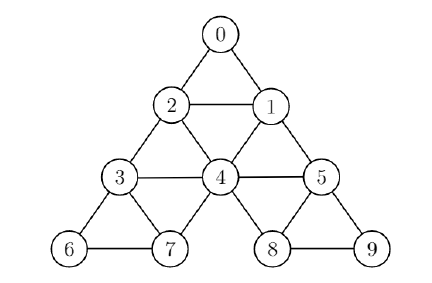
\includegraphics[width=0.4\textwidth]{grafo_formacion_triangular.png}
	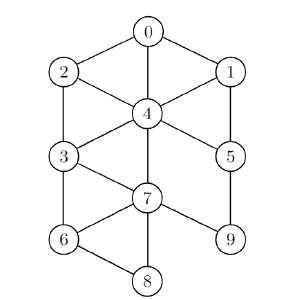
\includegraphics[width=0.4\textwidth]{grafo_formacion_hexagonal.png}
	\caption{Grafos de formación en triángulo y hexágono \cite{PenaAM_2019_tesis}.}
	\label{fig:grafos_formación}
\end{figure}

\subsection{Construcción de un grafo mínimamente rígido}
El método de Henneberg es utilizado para construir grafos mínimamente rígidos donde cada vértice mantiene dos grados de libertad \cite{KrickL_2007_tesis}. Los pasos para realizar el método son:

\begin{enumerate}
	\item Numerar todos los vértices.
	\item Agregar una arista entre el vértice 1 y el vértice 2.
	\item Agregan los demás vértices a la estructura utilizando dos aristas.
	\item Verificar que se cumple la condición de $e = \frac{v^2-v}{2}$
\end{enumerate}


\subsection{Grafo para la red de comunicación}
La comunicación entre agentes se representa por un grafo de comunicación. Este es un dígrafo que indica cuáles agentes tienen comunicación entre ellos y hacia qué dirección se comunican \cite{grafos_en_redes_multiagente}. A continuación se muestran tres tipos de redes.

\begin{itemize}
	\item Red estática: Las aristas se mantienen invariantes en el tiempo.
	\item Red dinámica o dependiente del estado: Las aristas son variantes en el tiempo y pueden desaparecer o aparecer según el estado de la red de agentes.
	\item Red aleatoria: La existencia de una arista se da mediante una distribución de probabilidad.
\end{itemize}

\section{Teoría de control}
En la robótica, se utilizan sistemas de control que integran varios subsistemas y procesos para estabilizar una respuesta inestable. Esto se logra mediante la implementación de un controlador que manipula las entradas del sistema para obtener la salida deseada \cite{control_lazo_cerrado}. En la Figura \ref{fig:lazo_cerrado_control} se muestra el sistema de control más utilizado.

\begin{figure}[H]
	\centering
	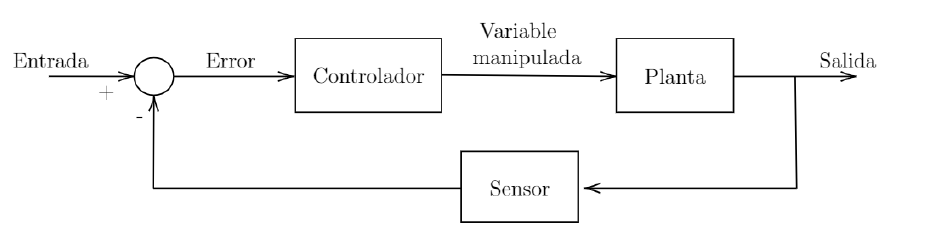
\includegraphics[width=0.8\textwidth]{lazo_cerrado_control.png}
	\caption{Sistema de control en lazo cerrado \cite{control_lazo_cerrado}.}
	\label{fig:lazo_cerrado_control}
\end{figure}

\subsection{Control de formación}
Para realizar el control de formaciones se requieren dos niveles de control, uno superior y otro inferior. El control de capa superior maneja el comportamiento de los agentes y sus posiciones. El control de capa inferior controla la velocidad de las ruedas en cada agente \cite{PenaAM_2019_tesis}.

\section{Cinemática de robots diferenciales con ruedas}
Para la implementación física en la robótica de enjambre se requiere un modelo de movimiento que contemple las dimensiones y características físicas del robot como se observa en la Figura \ref{fig:modelo_uniciclo}. Para esto se tienen las ecuaciones (\ref{eq:velocidad_lineal_uniciclo}) y (\ref{eq:velocidad_angular_uniciclo}). Donde $\ell$ es la distancia del motor hasta su centro, $\varphi$ es el ángulo de orientación del uniciclo dentro del plano $XY$, $v$ es la velocidad lineal del robot, $w$ es la velocidad angular de las ruedas y $r$ es el radio de las ruedas \cite{ZeaM_modelo_uniciclo}.

\begin{equation}
	v = \frac{r(\dot{\varphi}_R + \dot{\varphi}_L)}{2}
	\label{eq:velocidad_lineal_uniciclo}
\end{equation}

\begin{equation}
	w = \frac{r(\dot{\varphi}_R + \dot{\varphi}_L)}{2\ell}
	\label{eq:velocidad_angular_uniciclo}
\end{equation}

\begin{figure}[H]
	\centering
	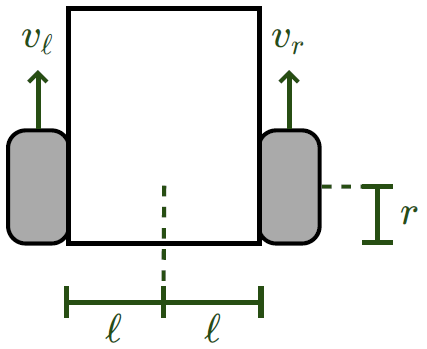
\includegraphics[width=0.5\textwidth]{modelo_uniciclo.png}
	\caption{Modelo de uniciclo \cite{ZeaM_modelo_uniciclo}.}
	\label{fig:modelo_uniciclo}
\end{figure}

Adicional a esto, se puede calcular la velocidad controlada de la rueda derecha y la rueda izquierda con las ecuaciones (\ref{eq:velocidad_controlada_derecha}) y (\ref{eq:velocidad_controlada_izquierda}), respectivamente.

\begin{equation}
	\dot{\varphi}_{R,crtl} = \frac{v_{ctrl} + \ell w_{crtl}}{r}
	\label{eq:velocidad_controlada_derecha}
\end{equation}

\begin{equation}
	\dot{\varphi}_{L,crtl} = \frac{v_{ctrl} - \ell w_{crtl}}{r}
	\label{eq:velocidad_controlada_izquierda}
\end{equation}

\section{Otras ecuaciones matemáticas relevantes}
Para mantener una correcta formación y distribución del enjambre, se necesitan herramientas como la ecuación de consenso y la función de tensión.

\subsection{Ecuación de consenso}
La ecuación (\ref{eq:consenso}) se utiliza para mantener la formación de los agentes en la posición asignada. Esta toma en cuenta el centro de masa de la formación y calcula la velocidad de cada agente para mantener la forma del grafo \cite{PenaAM_2019_tesis}.

\begin{equation}
	v_i(t) = \sum_{j \in N(i)} (x_j(t) - x_i(t)), i = 1, 2, ..., n
	\label{eq:consenso}
\end{equation}

Donde $N(i)$ es el conjunto de unidades adyacentes de la unidad $i$ en la red multi-agente.

Luego de añadir los pesos, se obtiene la ecuación (\ref{eq:consenso2}):

\begin{equation}
	\frac{\partial \varepsilon_{i,j}}{\partial x_i} = w_{i,j}(\Vert x_i - x_j \Vert)(x_i - x_j)
	\label{eq:consenso2}
\end{equation}

Donde de puede despejar el peso $w_{i,j}$.

\subsection{Funciones racionales para hallar la tensión}
Para modificar la ecuación de consenso es necesario hallar la tensión utilizando funciones racionales que toman en cuenta las distancias deseadas y las distancias restringidas \cite{PenaAM_2019_tesis}.

\begin{itemize}
	\item Modelo 1: Combinación aditiva del control de formación y evasión de obstáculos.
	\begin{equation}
		\epsilon_{ij} = \frac{1}{2}(\Vert x_i - x_j \Vert - d_{ij})^2 + \frac{\Vert x_i - x_j \Vert^2}{\Vert x_i - x_j \Vert - r}
		\label{eq:ConsensoModelo1}
	\end{equation}
	Donde, $d_{ij}$ es la distancia entre los agentes $i$ y $j$, y $r$ es el radio de los agentes.
	
	\item Modelo 2: Combinación de control de formación, evasión de obstáculos y mantenimiento de la conectividad.
	\begin{equation}
		\epsilon_{ij} = \frac{(\Vert x_i - x_j \Vert - d_{ij})^2}{(\Vert x_i - x_j \Vert - r)(\Vert x_i - x_j \Vert - R)}
		\label{eq:ConsensoModelo2}
	\end{equation}
	Donde, $R$ es la distancia máxima que se pueden alejar los agentes sin salirse del rango del radar de los otros.
	
	\item Modelo 3: Combinación de control de formación y evasión de obstáculos.
	\begin{equation}
		\epsilon_{ij} = \frac{2(\Vert x_i - x_j \Vert - d_{ij})^2}{\Vert x_i - x_j \Vert - r}
		\label{eq:ConsensoModelo3}
	\end{equation}
	
	\item Modelo 4: Modelo dinámico con control de formación y evasión de obstáculos.\par
	
	Se utiliza un modelo dinámico que al inicio, cuando los agentes comienzan en posiciones aleatorias, se utiliza únicamente el control para evitar colisiones. Luego, cuando los agentes están lo suficientemente cerca sin chocarse, se cambia al modelo de la ecuación (\ref{eq:ConsensoModelo3}) que toma en cuenta el control de la formación 
	
	\item Modelo 5: Modelo dinámico con control de formación usando coseno hiperbólico y evasión de obstáculos.
	\begin{equation}
		\epsilon_{ij} = 0.01\cosh{(1.8 \Vert x_i - x_j \Vert - 8.4)}
		\label{eq:ConsensoModelo5}
	\end{equation}
	Se utilizó el coseno hiperbólico ya que es una función ``plana'' que permite que el control de formación sea el que decida dónde deben posicionarse los agentes en caso de tener un mínimo erróneo en una distancia de 0.
	
	\item Modelo 6: Modelo dinámico con control de formación usando coseno hiperbólico y evasión de obstáculos incluyendo límites de velocidad.\par
	Esta modificación no afecta directamente a la ecuación. Se realiza después de esta y consiste en incluir un límite de velocidad al modelo de la ecuación (\ref{eq:ConsensoModelo5}). Por lo tanto, si la velocidad obtenida con el modelo es mayor al límite establecido, solo se tomará en cuenta la dirección.
	
\end{itemize}

\section{Herramientas de software}
Para realizar los cálculos, el control y las pruebas con los agentes robóticos, se necesita utilizar software especializado como los siguientes:

\subsection{Matlab}
Matlab es una plataforma de programación desarrollada por MathWorks con su propio lenguaje especializado para aplicaciones de ingeniería, análisis de datos, generación de algoritmos, entre otras \cite{matlab}.

Para el presente trabajo, se utiliza Matlab como la fuente de procesamiento de datos y generación de trayectorias para el algoritmo de sincronización y control de formaciones.

\subsection{Entorno de simulación Webots}
Webots es un software de código abierto creado por Cyberbotics \cite{webots}. Esta plataforma se centra en la simulación de escenarios que permiten replicar situaciones reales con distintos tipos de robots y objetos tal como se muestra en la Figura \ref{fig:webots}. Varios de los modelos disponibles en Webots están calibrados para comportarse como el modelo real y el usuario puede modificar los parámetros para garantizar una simulación realista.

Webots también cuenta con la implementación de controladores en lenguajes como C, C$++$, Matlab, Python, Java, ROS, o con API.

\begin{figure}[H]
	\centering
	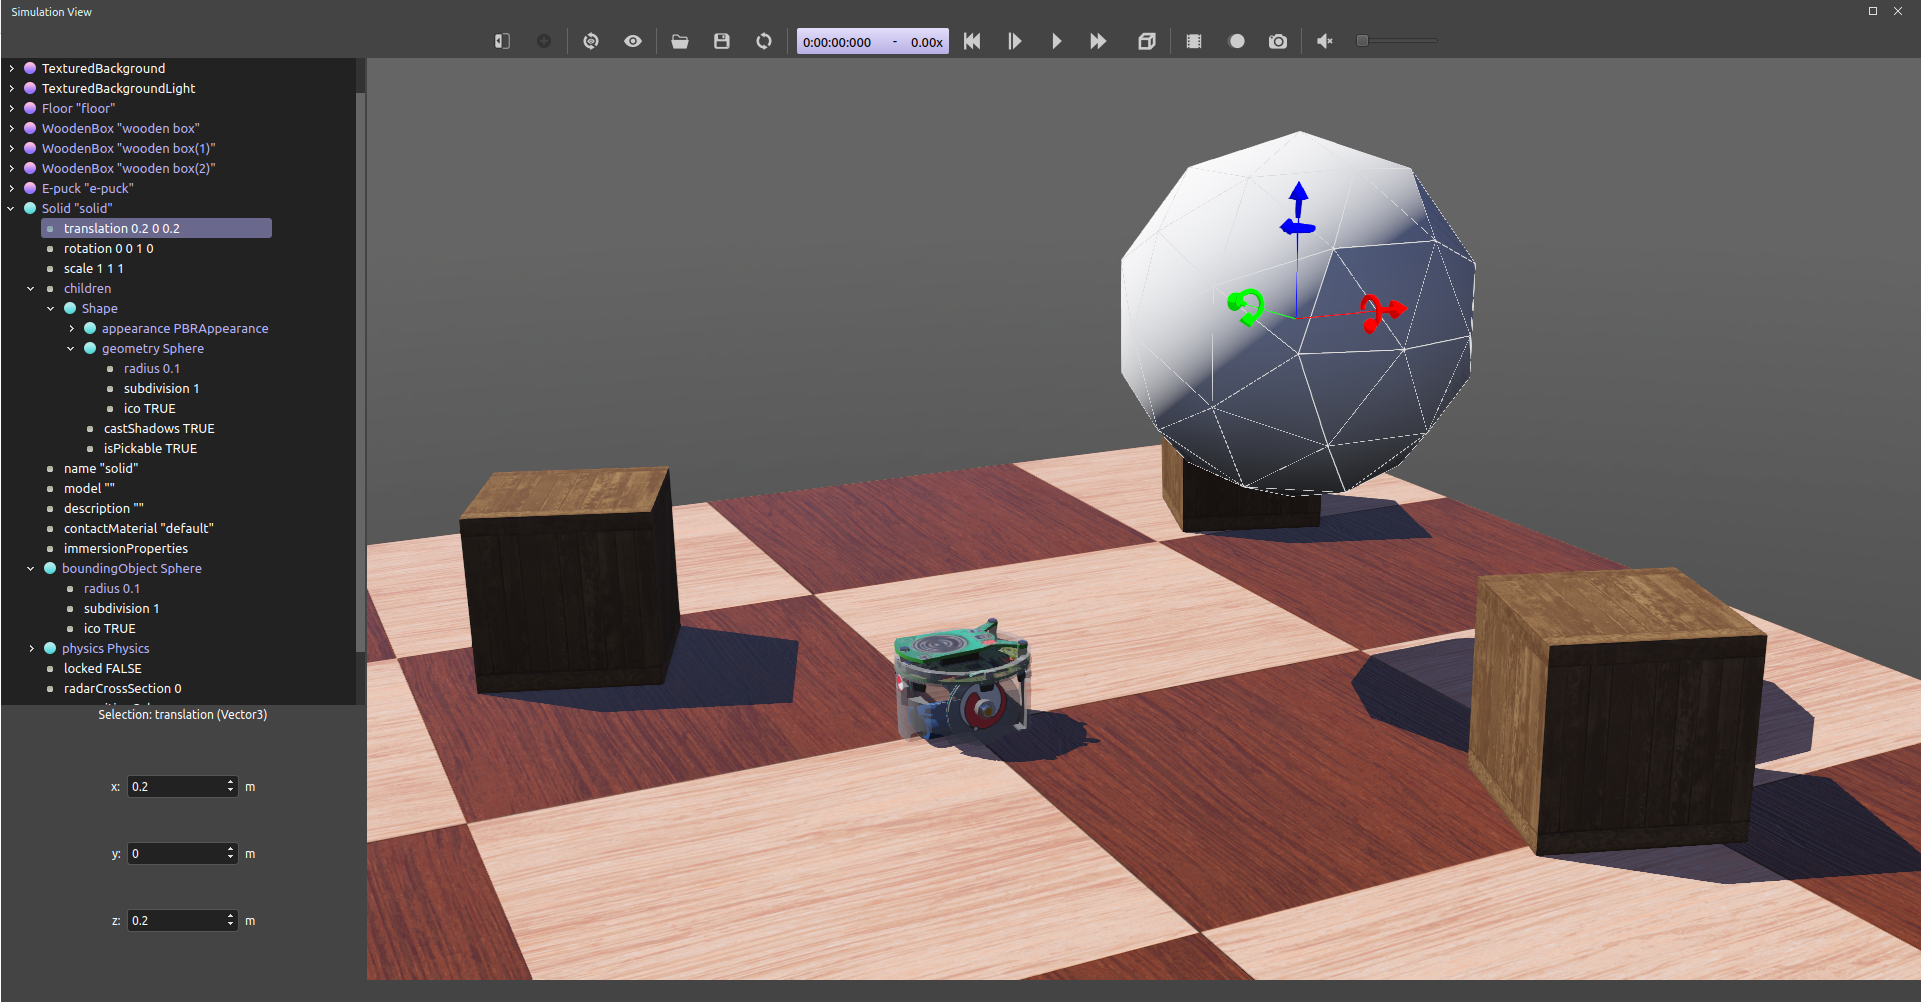
\includegraphics[width=0.8\textwidth]{webots.png}
	\caption{Entorno de simulación en Webots \cite{webots}.}
	\label{fig:webots}
\end{figure}

\subsection{Paralelismo computacional}
Al momento de trabajar con algoritmos y problemas complejos, se requiere utilizar métodos de optimización de software para agilizar el procesamiento de cálculos y la ejecución de tareas. 
Para esto, se utilizan herramientas como el paralelismo computacional. Consiste en dividir las tareas y asignarlas a cada núcleo del procesador para ejecutarlas simultáneamente \cite{libro_paralelismo}. Esto reduce considerablemente el tiempo de procesamiento. Además es importante considerar las dependencias entre las tareas como:

\begin{itemize}
	\item Dependencia de control de secuencia: Es el orden secuencial clásico de los algoritmos secuenciales.
	\item Dependencia de comunicación: Es cuando una tarea depende de la información que envíe otra tarea.
\end{itemize}

En la Figura \ref{fig:paralelismo_dependencia_tareas} se observa un ejemplo donde puede existir tiempos muertos ya que la tarea 3 depende de la información enviada por la tarea 1 y la tarea 4 depende de la información enviada por la tarea 3.
\begin{figure}[H]
	\centering
	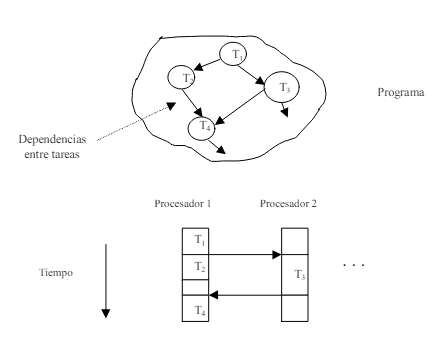
\includegraphics[width=0.6\textwidth]{paralelismo_dependencia_tareas.png}
	\caption{Ejemplo de dependencia de tareas \cite{libro_paralelismo}.}
	\label{fig:paralelismo_dependencia_tareas}
\end{figure}

\section{Ecosistema Robotat}
El Robotat es una plataforma que cuenta con herramientas y sistemas de captura de movimiento útiles para experimentar con la robótica de enjambre. A continuación se describen las herramientas más importantes.

\subsection{Mesa de pruebas}
Es una plataforma de acero y plycem con un espacio útil de $5 \times 5 \times 3$ m, capaz de soportar cargas puntuales de hasta dos toneladas. 

\subsection{Sistema de captura de movimiento OptiTrack}
Es un sistema de captura de movimiento que consta de 6 cámaras OptiTrack Prime$^x$ 41 al rededor de la mesa de pruebas. Estas son cámaras de alta precisión y baja latencia que permiten realizar experimentos en tiempo real. En la Figura \ref{fig:OptiTrack_primex41} se muestra el modelo disponible en la Universidad del Valle de Guatemala que tiene las siguientes características \cite{primex41}:

\begin{itemize}
	\item Resolución de 4.1 mega píxeles (MP).
	\item Precisión de $\pm$ 0.10 mm.
	\item Errores rotacionales menores a 0.5 grados.
	\item Lentes de 12 mm.
	\item Tasa de refresco nativa de 180 FPS con un un máximo de hasta 250 FPS.
	\item Distancia de captura de hasta 100 pies desde la cámara al marcador.
	\item Rango de captura de hasta 290,000 pies cúbicos por cámara para marcadores pasivos
	\item Rango de captura de hasta 1,000,000 pies cúbicos por cámara para marcadores activos.
\end{itemize}

\begin{figure}[H]
	\centering
	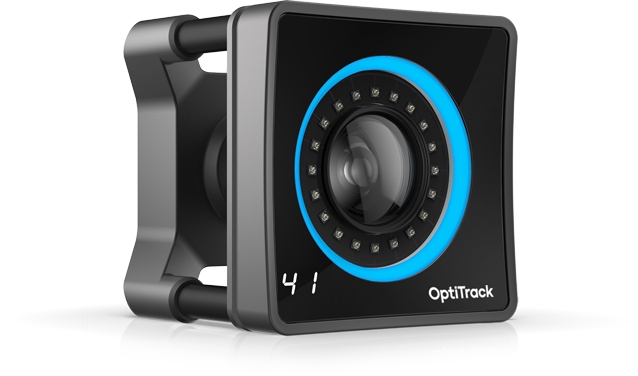
\includegraphics[width=0.5\textwidth]{primex41.png}
	\caption{Cámara de captura de movimiento Prime$^x$ 41 de OptiTrack \cite{primex41}.}
	\label{fig:OptiTrack_primex41}
\end{figure}

\subsection{Comunicación del Robotat}
La plataforma del Robotat utiliza un protocolo de comunicación TCP para transmitir la información de las cámaras OptiTrack al servidor principal del laboratorio. Este servidor de Python envía los datos a través de Wi-Fi en una red local. A esta red local, se puede acceder con una computadora para extraer la información que se necesite, además las plataformas robóticas también se pueden conectar a la red local para recibir instrucciones.

\section{Hardware}
Para poner a prueba el algoritmo de sincronización y control de formaciones en un ambiente físico, se necesita de una plataforma robótica móvil que en este proyecto será el Pololu 3pi+. 

\subsection{Plataforma móvil Pololu 3pi+ modificado}
La plataforma móvil a utilizar es una modificación basada en el Pololu 3pi+ 32U4 OLED Robot \cite{pololu3pi+}. Tiene un diámetro de 97 mm y altura de 36 mm, además, cuenta con lo siguiente:
\begin{itemize}
	\item Procesador ATmega34U4 MCU @ 16 MHz.
	\item Sensores de línea y de choque frontales.
	\item Encoders de doble cuadratura para control de posición y velocidad en lazo cerrado.
	\item IMU (acelerómetro de 3 ejes, magnetómetro y giroscopio).
	\item Pantalla OLED integrada.
\end{itemize}

\begin{figure}[H]
	\centering
	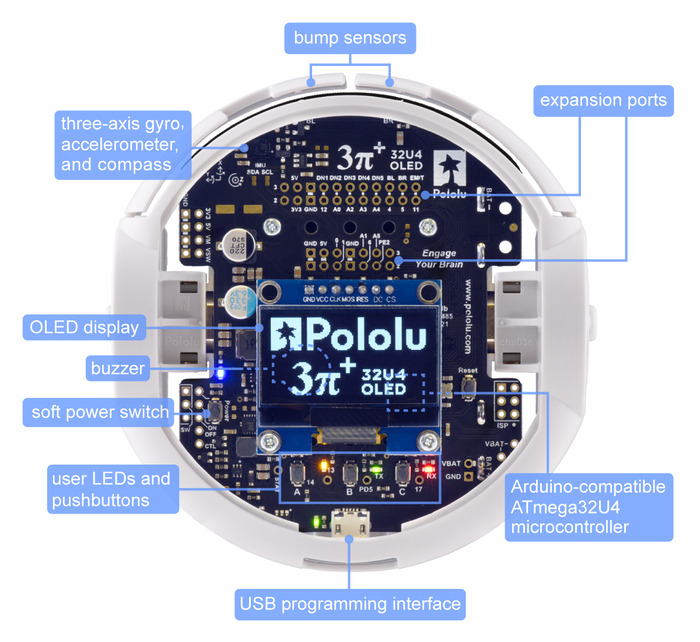
\includegraphics[width=0.45\textwidth]{pololu_sensores1.jpg} 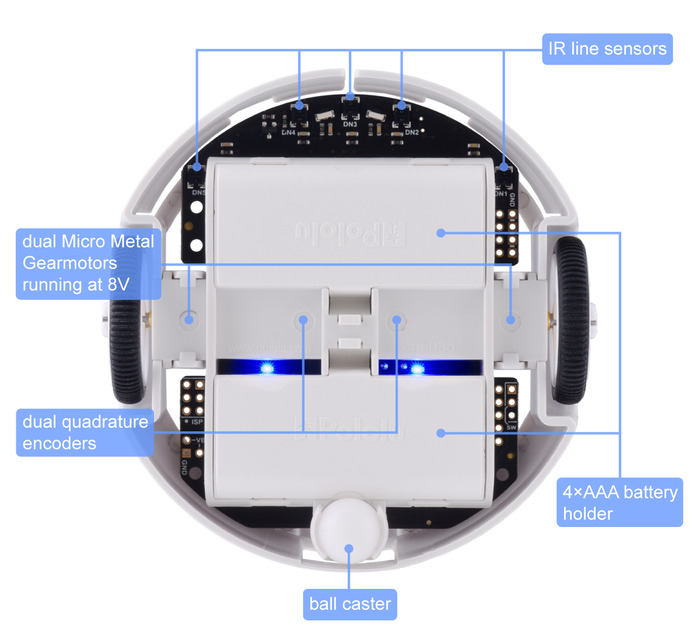
\includegraphics[width=0.45\textwidth]{pololu_sensores2.jpg}
	\caption{Sensores y componentes del Pololu 3pi+ 32U4 OLED Robot \cite{pololu3pi+}.}
	\label{fig:pololu_sensores}
\end{figure}

A esta plataforma móvil se le adaptó un ESP32 ya que el microcontrolador original tiene poca capacidad de procesamiento. Esto permitió tener control de capa superior e inferior, además de incorporar una red de comunicación WiFi con el Robotat para controlar los agentes.









	\fi
\fi

% CAPÍTULOS
% ------------------------------------------------------------------------------
\newpage
\ifdefined\parpordefecto
	\defaultparformat{j-capitulos}
\else
	\chapter{Algoritmo de sincronización y control de formaciones}
El algoritmo de sincronización y control de formaciones funciona con dos controladores principales. El primero es el algoritmo de sincronización y control centralizado llamado ``supervisor'' y el segundo es el algoritmo de control de uniciclo para los agentes. En este capítulo se explicará el funcionamiento de cada controlador y la lógica detrás de cada uno para cumplir con las tareas de formación, evasión de colisiones y movilización hacia un objetivo.

\subsection{Controlador del supervisor}
El programa del supervisor tiene como tarea coordinar a los agentes, realizar procesamiento de datos y generar trayectorias para movilizar a los agentes hacia un objetivo evadiendo colisiones entre ellos y con los obstáculos. Para esto, el algoritmo cuenta con diferentes segmentos.

\subsubsection{Adquisición de posiciones}
La primera parte del algoritmo consiste en la toma de posiciones $X$ y $Y$ actuales de los agentes, obstáculos y el objetivo. 

\subsubsection{Cálculo de velocidades de agentes}
Luego, se realiza el cálculo de las velocidades de los agentes para moverlos hacia su posición en la formación y hacia el objetivo de interés. Este cálculo de velocidades se realiza por medio de la ecuación de consenso con un factor de peso $\omega$ que depende de las ecuaciones de tensión y de evasión de obstáculos. 

\subsubsection{Evasión de obstáculos y colisiones}
Seguido a esto, se tiene la evasión de obstáculos y colisiones que se realiza comparando la posición actual de cada agente con la posición actual de los agentes vecinos y los obstáculos.

\subsubsection{Control proporcional}
El siguiente segmento implementa el control proporcional de la Ecuación (\ref{eq:controlador_proporcional}) para movilizar a los agentes hacia un punto de interés.

\begin{equation}
	v_{n+1} = v_n + k(x_{objetivo} - x_{agente})
	\label{eq:controlador_proporcional}
\end{equation}

Donde $v$ es la velocidad del agente y $k$ es la ganancia o constante de proporcionalidad que multiplica a la distancia entre el punto de interés y la posición del agente a evaluar. Una vez se tiene la velocidad en $X$ y $Y$ de los agentes, se calcula la norma de velocidad y esta se utiliza para la toma de decisiones dentro del algoritmo.

\subsection{Controlador de los agentes}
El programa del los agentes recibe las velocidades calculadas por el supervisor. Luego, se encarga de convertirlas en velocidad lineal y angular para calcular la velocidad de cada rueda de los Pololu 3Pi+ según el modelo del uniciclo. Este programa es individual para cada agente y solo procesa los datos para si mismo.

\subsection{Funcionamiento del algoritmo}
El algoritmo consta de las siguientes etapas para su ejecución:
\begin{itemize}
	\item Etapa 0: los agentes se movilizan hacia sus posiciones iniciales para iniciar el experimento.
	\item Etapa 1: comienza el acercamiento de agentes hasta que la norma de velocidad esté por debajo de un valor seleccionado.
	\item Etapa 2: los agentes se colocan en sus posiciones de la formación hasta que el error cuadrático medio entre la formación actual y la formación deseada esté por debajo de un valor seleccionado.
	\item Etapa 3: el líder se mueve hacia el objetivo y los agentes de la formación lo siguen.
\end{itemize}

En las Figuras \ref{fig:diagrama_supervisor} y \ref{fig:diagrama_agentes} se muestra el diagrama de flujo para los programas del supervisor y el control de los agentes.

\begin{figure}[H]
	\centering
	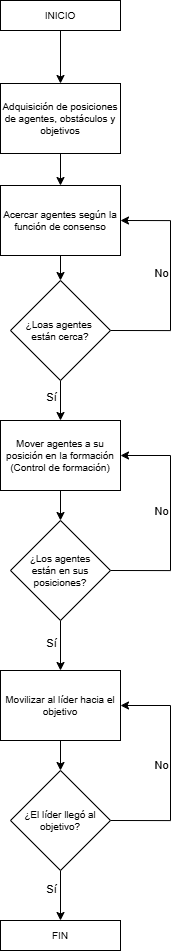
\includegraphics[width=0.25\textwidth]{optimizacion/diagrama_supervisor.png}
	\caption{Diagrama de flujo para el supervisor.}
	\label{fig:diagrama_supervisor}
\end{figure}

\begin{figure}[H]
	\centering
	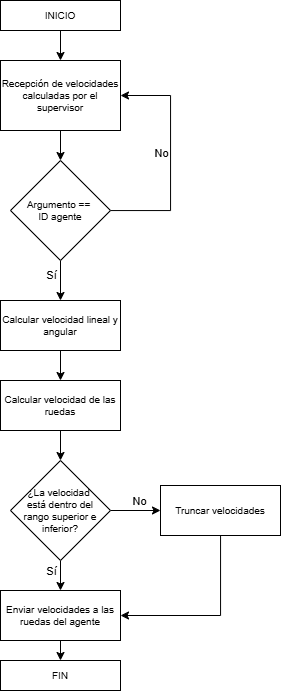
\includegraphics[width=0.5\textwidth]{optimizacion/diagrama_agentes.png}
	\caption{Diagrama de flujo para el programa de los agentes.}
	\label{fig:diagrama_agentes}
\end{figure}


\chapter{Restauración del algoritmo desarrollado en fases previas}
La implementación en físico del algoritmo de sincronización y control de formaciones llevada a cabo por José Alejandro Rodríguez \cite{RodriguezJA_2023_tesis} se realizó en Webots con la versión 2023b. Esta es la misma versión que la utilizada en la fase actual. También, se optó por utilizar Python 3.10 como lenguaje de programación para el controlador del supervisor y de los agentes ya que es una de las versiones más recientes de software, además que es la misma versión utilizada en la fase anterior. 

Por otro lado, en el Robotat se han realizado cambios en las conexiones con el servidor y los Pololu 3Pi+	por lo que se sería necesario un reajuste de parámetros.

En este capítulo se detallarán las modificaciones necesarias para la restauración del algoritmo y su correcta ejecución en simulaciones con Webots y en un entorno físico con el Robotat. Además, se realizará la validación de la naturaleza del algoritmo en escenarios con obstáculos móviles.


\section{Replicar simulaciones de Webots}
El primer paso de la restauración, fue recrear algunas simulaciones en Webots. Para esto, fue necesario instalar las siguientes librerías que no se encuentran dentro de la biblioteca estándar de Python:

\begin{itemize}
	\item Keyboard - versión 0.13.5
	\item NumPy - versión 1.23.2
\end{itemize}

Luego, se realizó la prueba del código para el controlador del supervisor y los agentes incluyendo sus respectivas funciones:
\begin{itemize}
	\item Supervisor: Supervisor\_simulacion\_y\_fisico\_v4.py
	\item Agentes: pruebaMatrizDifeomorfismo.py
	\item Funciones algoritmo: funciones.py, funVel.py
\end{itemize} 

\subsection{Comunicación entre supervisor y agentes}
Al ejecutar la primera simulación, se encontró que dos agentes permanecían inmóviles durante la primera etapa del algoritmo que consiste en mover a los agentes a sus posiciones iniciales, tal como se muestra en la Figura \ref{fig:delaygpu}.

\begin{figure}[H]
	\centering
	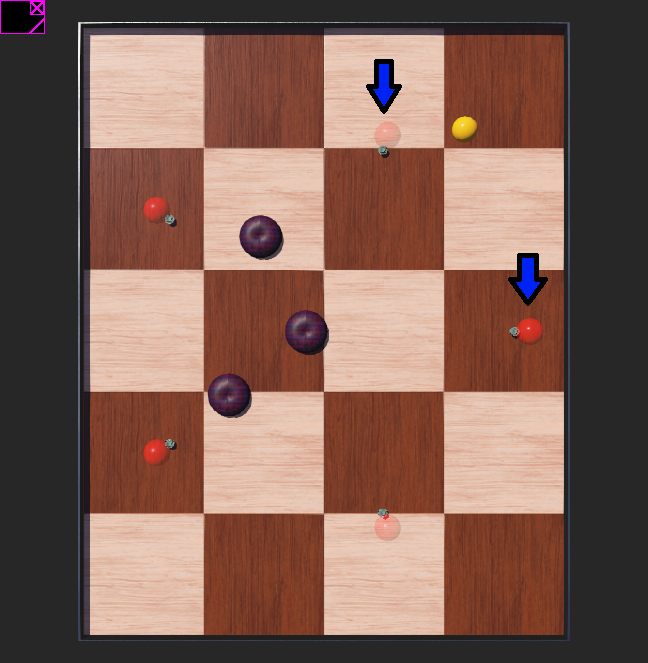
\includegraphics[width=0.30\textwidth]{replicar_webots/delaygpu_v2_1.png}
	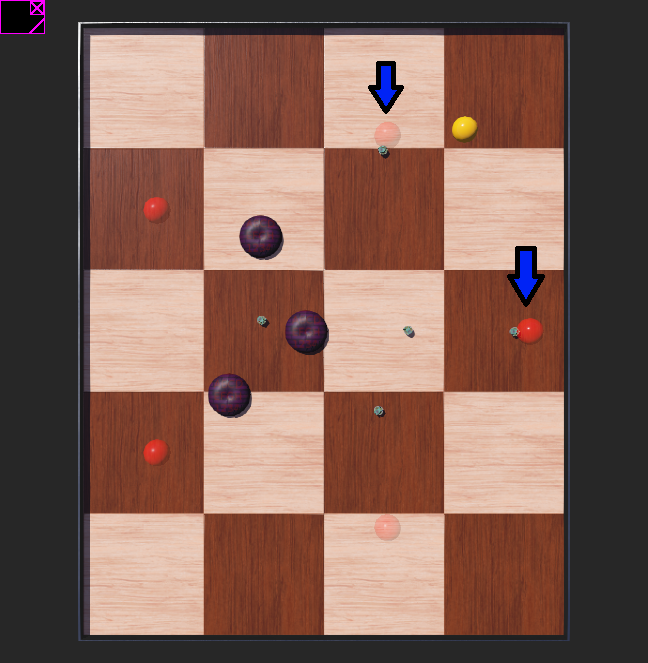
\includegraphics[width=0.30\textwidth]{replicar_webots/delaygpu_v2_2.png}
	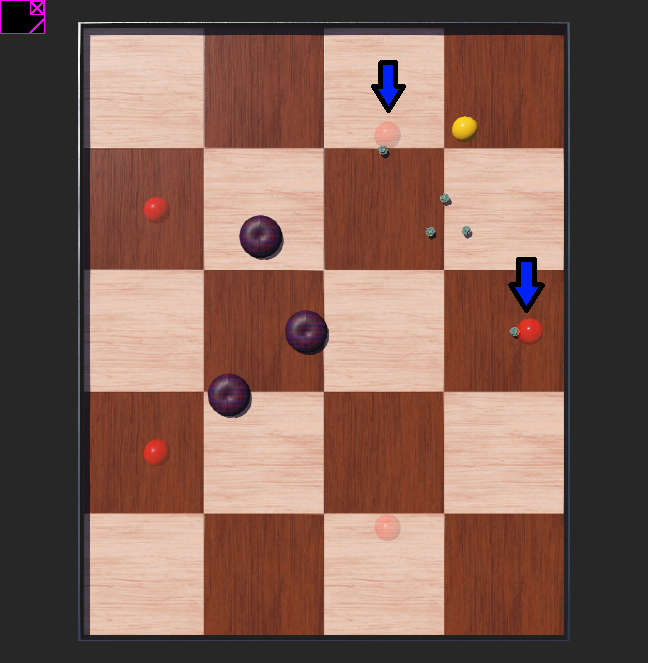
\includegraphics[width=0.30\textwidth]{replicar_webots/delaygpu_v2_3.png}
	\caption{Ejecución de la primera simulación en Webots 2023b.}
	\label{fig:delaygpu}
\end{figure}

Esto se debe a que actualmente se está utilizando una computadora con mayor capacidad de procesamiento que la utilizada en la fase anterior. Esta capacidad de procesamiento impacta en la velocidad de ejecución de los programas. 

Dado que la comunicación entre el supervisor y los agentes se realiza por medio de una memoria compartida y la velocidad de procesamiento es mayor, el controlador de los dos primeros agentes se ejecuta antes de que el espacio de memoria compartida se haya inicializado correctamente. Para solucionar el problema, en el controlador de los agentes se agregó un tiempo de espera de 3 segundos antes de inicializar y acceder a la memoria compartida para asegurar que esta se cree correctamente en el controlador del supervisor.

\subsection{Prueba del algoritmo con simulaciones basadas en escenarios previos}
Una vez solucionado el problema de comunicación, se realizó las primeras simulaciones para replicar algunos de los escenarios realizados por José Alejandro Rodríguez \cite{RodriguezJA_2023_tesis} y comprobar el funcionamiento correcto del algoritmo. 

El código del supervisor ya cuenta con un modo de simulación en el que se ejecuta el algoritmo basado en condiciones iniciales tomadas de un escenario físico. Para esto, se debe cargar un archivo .npz que cuenta con la información necesaria para configurar la simulación según el escenario real en que se ejecutó el algoritmo.

\subsubsection{Primer escenario}
Para la primera simulación, se utilizó el archivo ``finaltrial\_6A\_AAA\_f\_1.npz'' que consiste en la siguiente configuración:

\begin{itemize}
	\item Cantidad de agentes: 6
	\item Posición inicial de agentes: línea
	\item Obstáculos: ninguno
	\item Objetivo: ubicado en la esquina
\end{itemize}

En la Figura \ref{fig:primera_simulacion}, las imágenes en el orden de izquierda a derecha y luego de arriba hacia abajo muestran la secuencia de ejecución del algoritmo.

\begin{figure}[H]
	\centering
	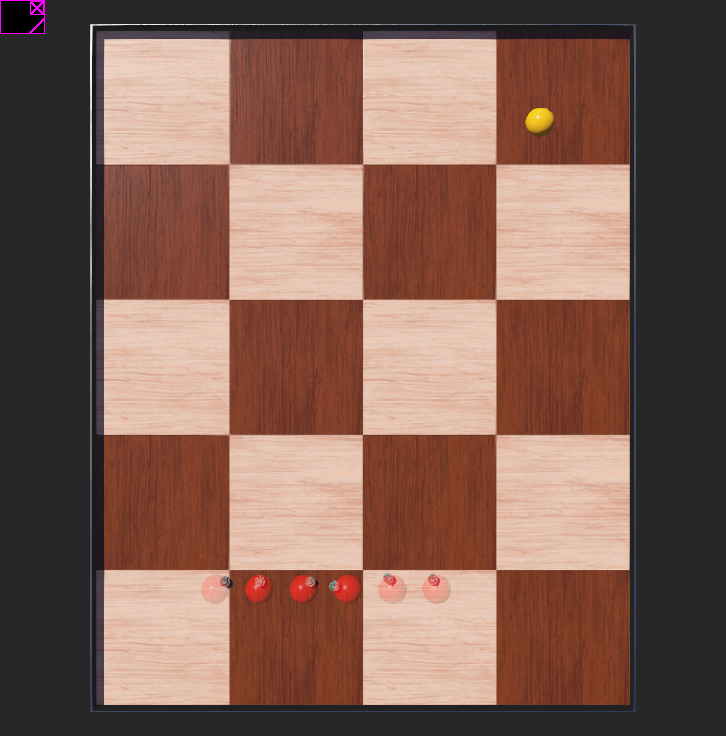
\includegraphics[width=0.45\textwidth]{replicar_webots/sim1_p1.png}
	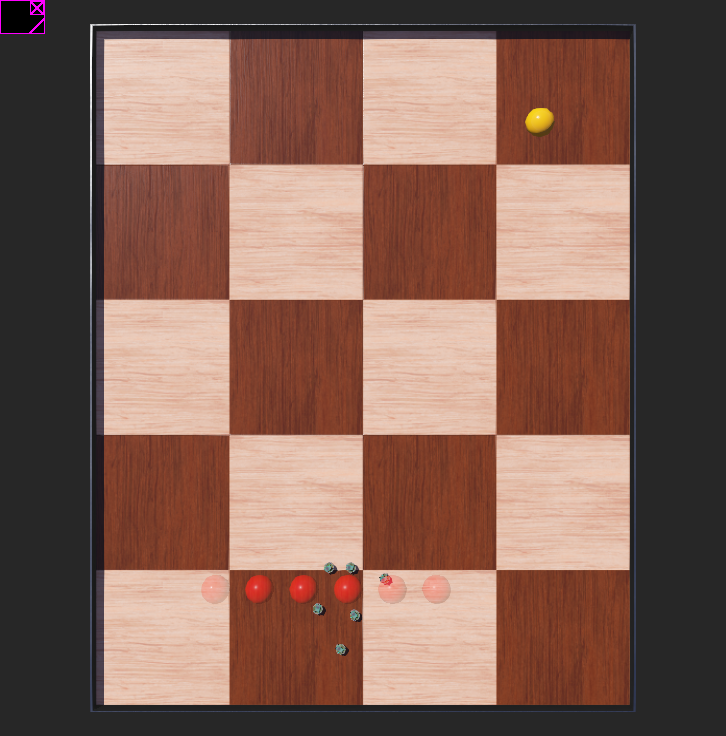
\includegraphics[width=0.45\textwidth]{replicar_webots/sim1_p2.png}
	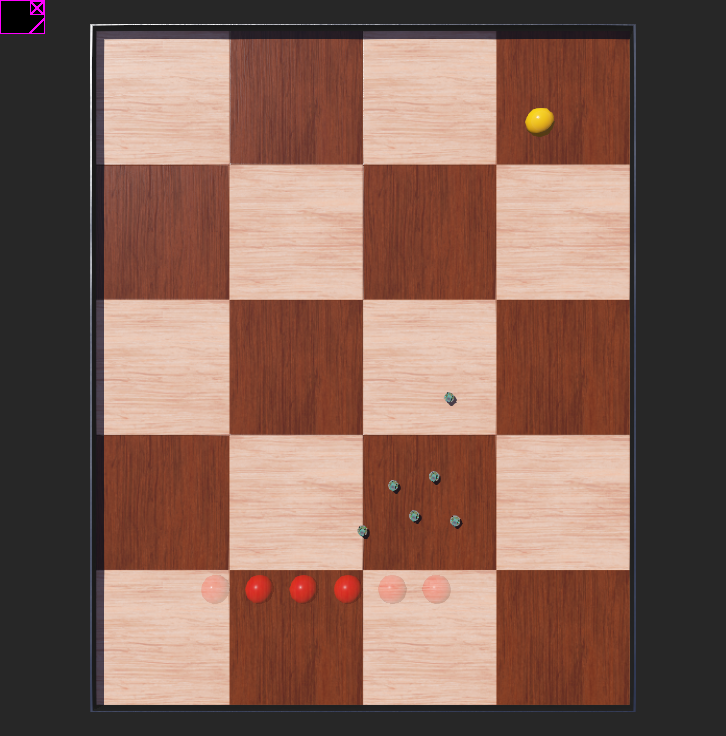
\includegraphics[width=0.45\textwidth]{replicar_webots/sim1_p3.png}
	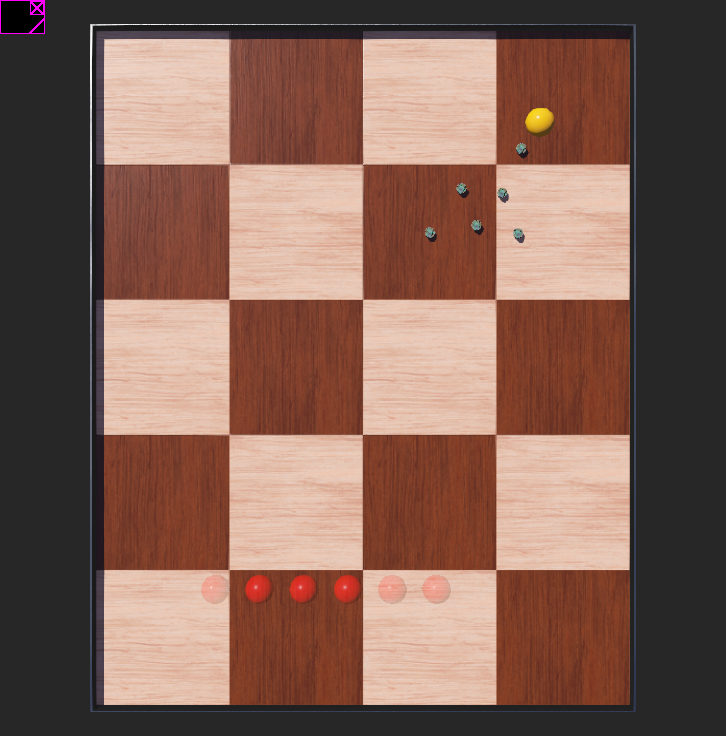
\includegraphics[width=0.45\textwidth]{replicar_webots/sim1_p4.png}
	\caption{Ejecución del algoritmo en la primera simulación}
	\label{fig:primera_simulacion}
\end{figure}

\subsubsection{Segundo escenario}
Para la segunda simulación, se utilizó el archivo ``finaltrial\_6A\_AB1B\_f\_2.npz'' que consiste en la siguiente configuración:

\begin{itemize}
	\item Cantidad de agentes: 6
	\item Posición inicial de agentes: línea
	\item Obstáculos: ubicados en el centro
	\item Objetivo: ubicado en el centro
\end{itemize}

En la Figura \ref{fig:segunda_simulacion}, las imágenes en el orden de izquierda a derecha y luego de arriba hacia abajo muestran la secuencia de ejecución del algoritmo.

\begin{figure}[H]
	\centering
	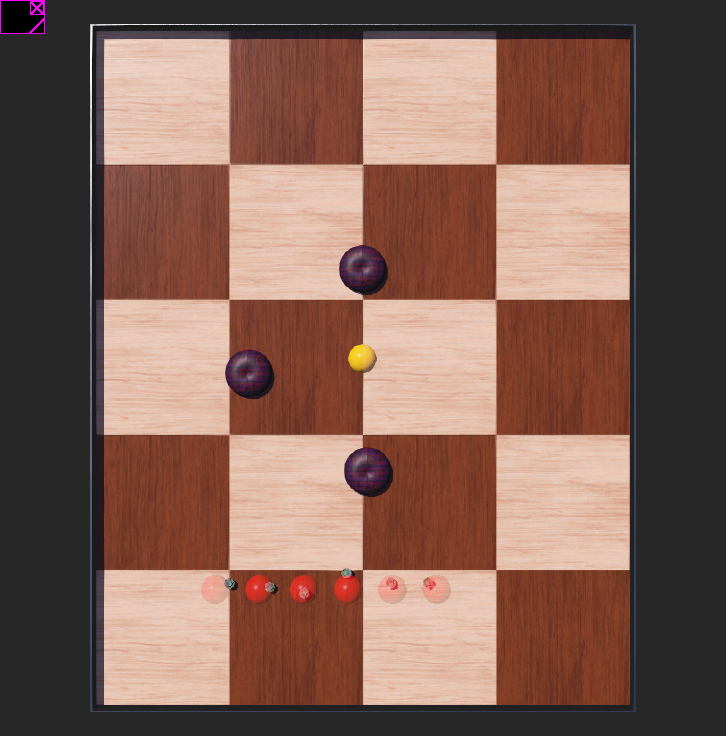
\includegraphics[width=0.45\textwidth]{replicar_webots/sim2_p1.png}
	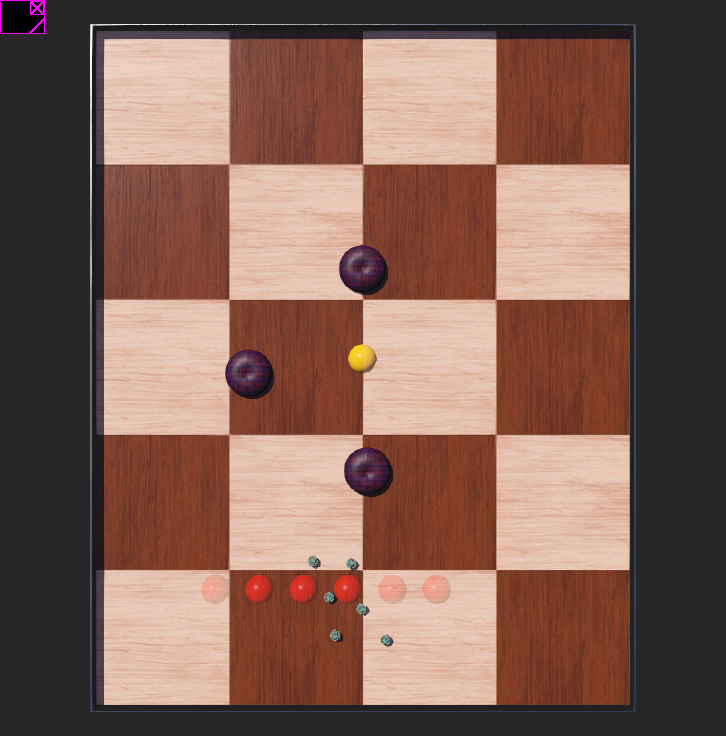
\includegraphics[width=0.45\textwidth]{replicar_webots/sim2_p2.png}
	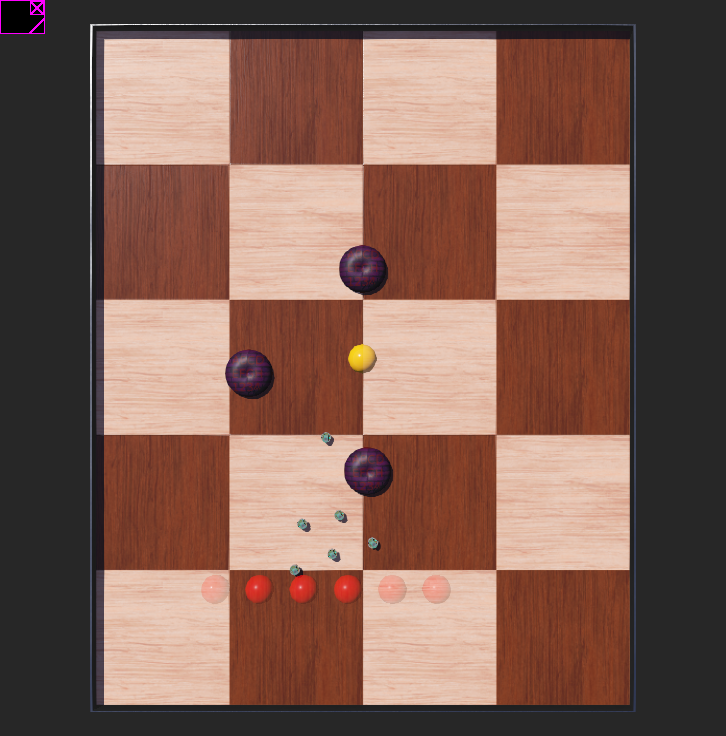
\includegraphics[width=0.45\textwidth]{replicar_webots/sim2_p3.png}
	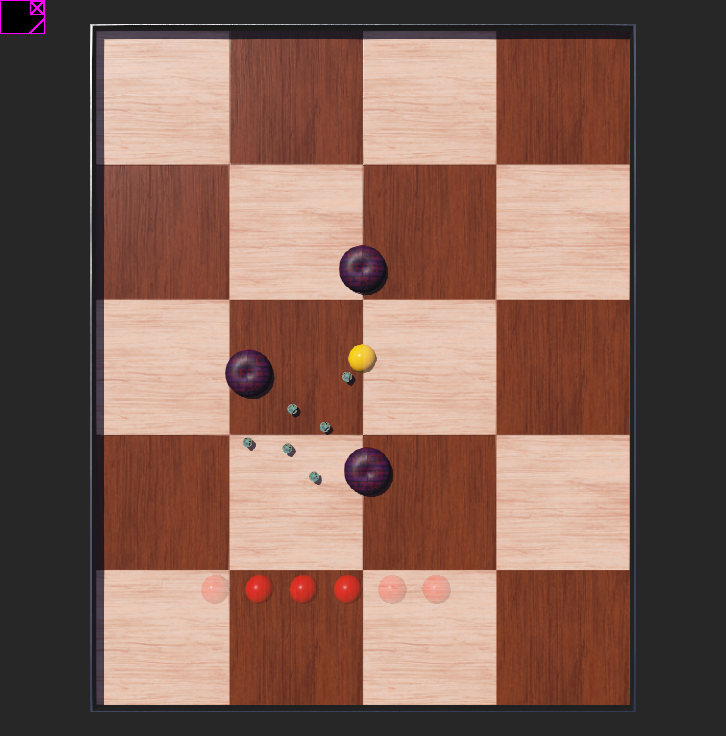
\includegraphics[width=0.45\textwidth]{replicar_webots/sim2_p4.png}
	\caption{Ejecución del algoritmo en la segunda simulación}
	\label{fig:segunda_simulacion}
\end{figure}

\subsubsection{Tercer escenario}
Para la tercera simulación, se utilizó el archivo ``finaltrial\_6A\_BCA\_f\_1.npz'' que consiste en la siguiente configuración:

\begin{itemize}
	\item Cantidad de agentes: 6
	\item Posición inicial de agentes: círculo
	\item Obstáculos: ubicados en posiciones aleatorias
	\item Objetivo: ubicado en la esquina
\end{itemize}

En la Figura \ref{fig:tercera_simulacion}, las imágenes en el orden de izquierda a derecha y luego de arriba hacia abajo muestran la secuencia de ejecución del algoritmo.

\begin{figure}[H]
	\centering
	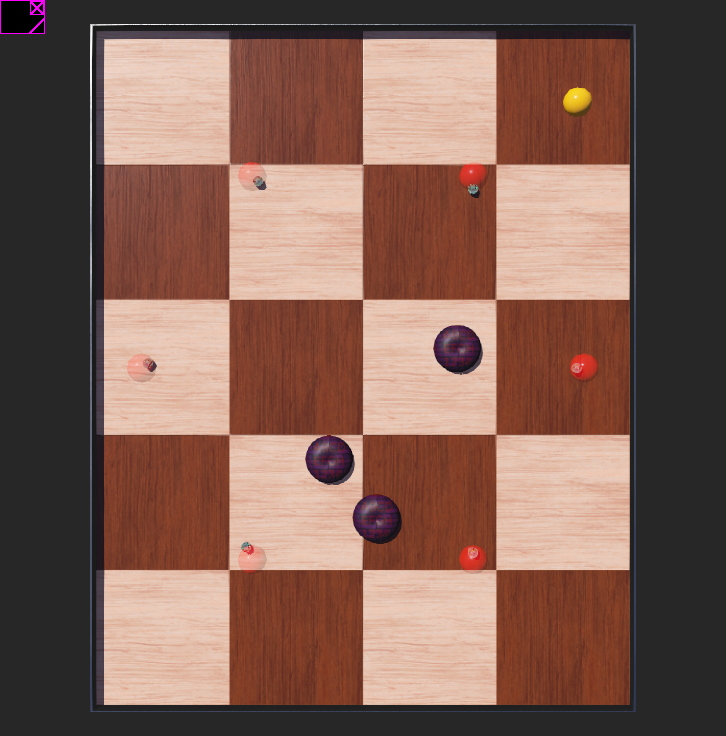
\includegraphics[width=0.45\textwidth]{replicar_webots/sim3_p1.png}
	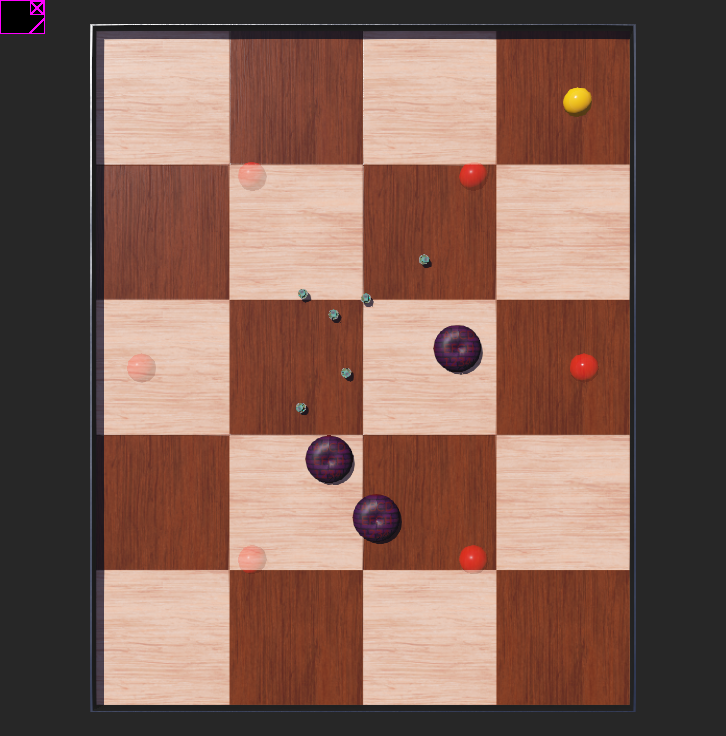
\includegraphics[width=0.45\textwidth]{replicar_webots/sim3_p2.png}
	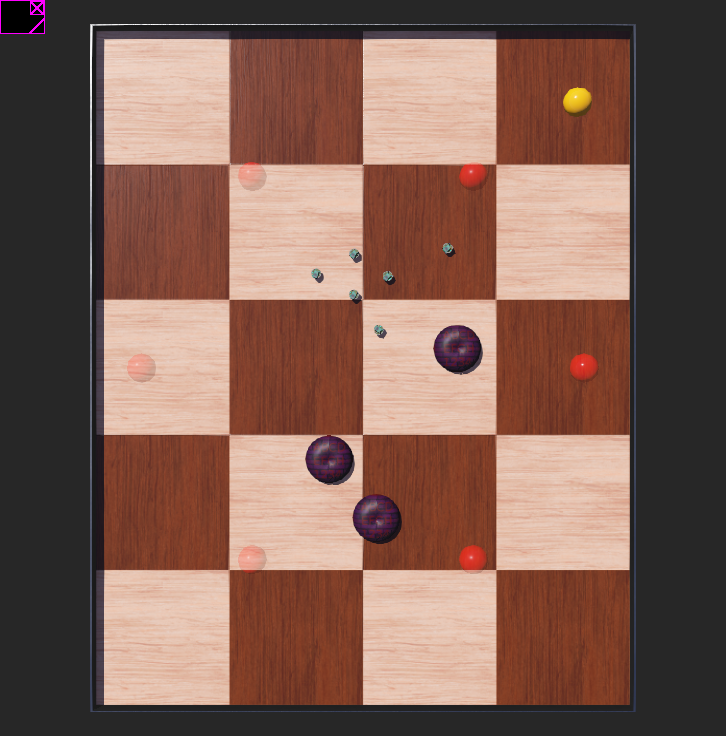
\includegraphics[width=0.45\textwidth]{replicar_webots/sim3_p3.png}
	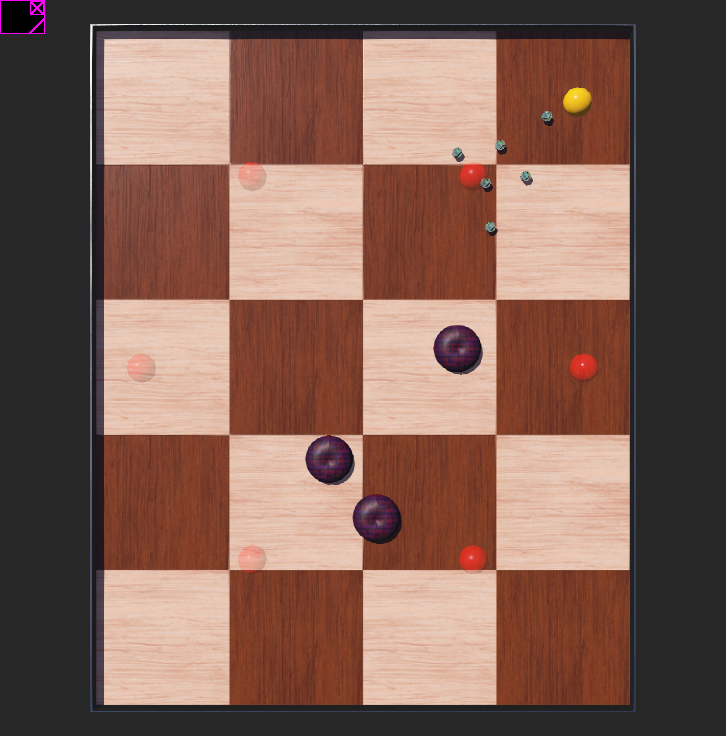
\includegraphics[width=0.45\textwidth]{replicar_webots/sim3_p4.png}
	\caption{Ejecución del algoritmo en la tercera simulación}
	\label{fig:tercera_simulacion}
\end{figure}

\section{Replicar el funcionamiento del algoritmo en el Robotat}
Una vez teniendo el algoritmo funcionando en Webots, el siguiente paso fue verificar que el algoritmo se ejecute correctamente en el Robotat.

\subsection{Pruebas de conexión con el Pololu 3Pi+ y el Robotat}
 Primero, se realizaron pruebas de conexión y obtención de datos con el Robotat y los Pololu 3Pi+ utilizando las funciones creadas en Python por José Alejandro Rodríguez \cite{RodriguezJA_2023_tesis}:
 
\begin{itemize}
	\item robotat\_connect
	\item robotat\_disconnect
	\item robotat\_get\_pose
	\item robotat\_3pi\_connect
	\item robotat\_3pi\_disconnect
	\item robotat\_3pi\_set\_wheel\_velocities
	\item robotat\_3pi\_force\_stop
\end{itemize}

Al realizar las pruebas de conexión con los agentes Pololu 3Pi+ se tenía el error mostrado en la Figura \ref{fig:error_conexion}. Este error se debe a que hubo un cambio en los puertos de conexión con el ESP$32$ de los agentes. Anteriormente la conexión se realizaba en el puerto $8888$ y actualmente se realiza en el puerto $9090$. Al actualizar este dato dentro de la función ``robotat\_3pi\_connect''  en del archivo ``funciones\_conjunto\_3pi.py'' se logró una conexión exitosa con el agente para el envío de comandos de velocidades.

\begin{figure}[H]
	\centering
	
\includegraphics[width=0.8\textwidth]{replicar_fisico_pruebas/error_conexion.png}
	\caption{Error de conexión con Pololu 3Pi+.}
	\label{fig:error_conexion}
\end{figure}

\subsection{Calibración de marcadores}
Una vez lograda la conexión con los Pololu 3Pi+, se tuvo que realizar una nueva calibración de los marcadores del OptiTrack para obtener el desfase del ángulo orientación (\textit{bearing}) de cada marcador. Estos desfases son diferentes en cada marcador y se producen por la forma en que el OptiTrack identifica cada uno según la posición de sus esferas reflectivas.

En la fase anterior, se realizó una calibración con los marcadores del $1$ al $15$, sin embargo, se agregaron nuevos marcadores por lo que ahora se cuenta con $22$ de ellos para utilizar, de los cuales están inhabilitados el $1$ y $9$ ya que serán utilizados en otros proyectos de graduación. Por tanto, ahora se tienen disponibles los marcadores de la Figura \ref{fig:marcadores_disponibles}. 

Para corregir el desfase de cada marcador, primero se obtiene la orientación con ángulos de Euler en la secuencia $zyx$, luego, al primer ángulo que representa la rotación respecto al eje $z$ se le resta el desfase obtenido $\theta_z$. Para realizar la calibración, se colocaron todos los marcadores disponibles de la Figura \ref{fig:marcadores_disponibles} con la misma orientación sobre el eje $y$ de la mesa de pruebas del Robotat tal como se observa en la Figura \ref{fig:marcadores_calibracion}.

\begin{figure}[H]
	\centering
	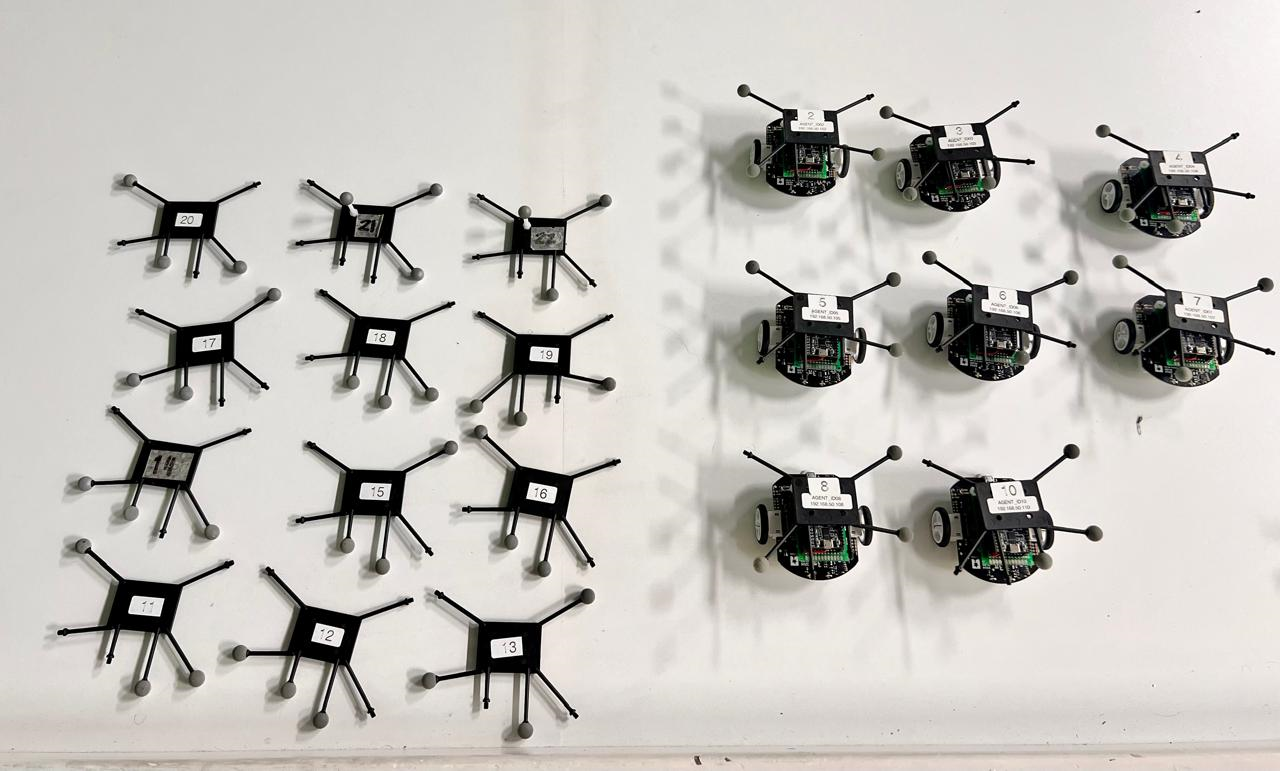
\includegraphics[width=0.8\textwidth]{replicar_fisico_pruebas/marcadores_disponibles.png}
	\caption{Marcadores del OptiTrack disponibles para su uso.}
	\label{fig:marcadores_disponibles}
\end{figure}

\begin{figure}[H]
	\centering
	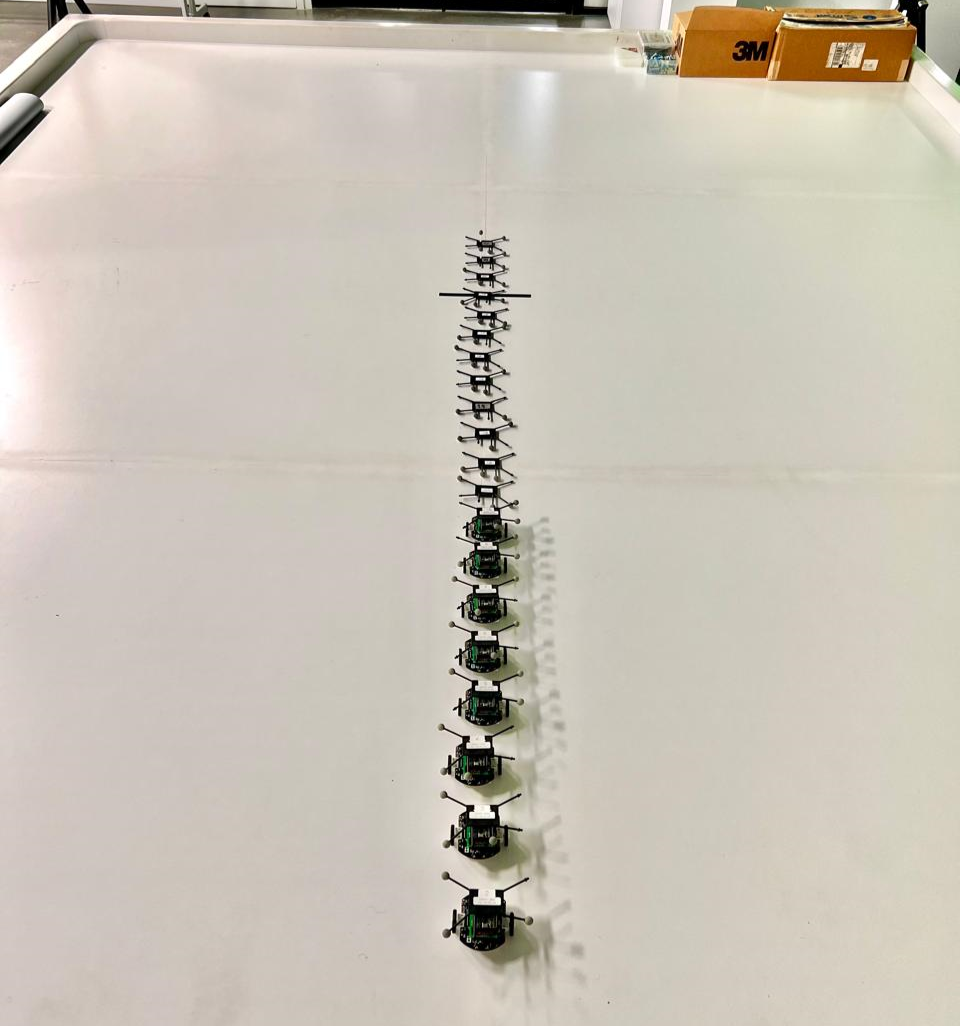
\includegraphics[width=0.6\textwidth]{replicar_fisico_pruebas/marcadores_ejey.png}
	\caption{Marcadores alineados sobre el eje $y$ de la mesa de pruebas del Robotat.}
	\label{fig:marcadores_calibracion}
\end{figure}

Al obtener la pose de cada marcador, se realizó la conversión a ángulos de Euler en la secuencia $zyx$ y se obtuvo los ángulos de desfase del Cuadro \ref{cuadro:desfases_iniciales}. Al comparar los desfases actuales con los obtenidos en la fase previa mostrados en el Cuadro \ref{cuadro:desfases_anteriores}, se observó que los valores son similares por lo que se optó tomar los desfases anteriores para los marcadores $1$ y $9$ faltantes en la calibración actual. Por último, en el Cuadro \ref{cuadro:desfases_finales} se observan los desfases finales para cada uno de los marcadores del $1$ al $22$. Estos valores se guardaron en un archivo .npy llamado ``nueva\_calibracion\_markers\_1\_al\_22.npy'' para aplicarlos luego de obtener la pose de cada marcador en el algoritmo y así tener siempre un ángulo respecto del eje $z$ igual a cero ($\theta_z$ = 0).

\begin{table}[H]
	\centering
	\begin{tabular}{|l|l|}
		\hline
		\textbf{Marcador} & \textbf{Desfase  $\theta_z$ en grados} \\ \hline
		2 & -47.2746822 \\ \hline
		3 & -90.32278167 \\ \hline
		4 & -135.7890952 \\ \hline
		5 & 179.3715195 \\ \hline
		6 & -141.0274548 \\ \hline
		7 & -175.0541793 \\ \hline
		8 & -78.11543097 \\ \hline
		10 & 143.2079276 \\ \hline
		11 & 111.0832797 \\ \hline
		12 & 166.1718189 \\ \hline
		13 & -127.3111755 \\ \hline
		14 & -109.4993486 \\ \hline
		15 & -40.73944282 \\ \hline
		16 & -104.1691129 \\ \hline
		17 & -121.1927571 \\ \hline
		18 & -92.48122033 \\ \hline
		19 & 4.298050244 \\ \hline
		20 & -133.2161012 \\ \hline
		21 & -112.0477043 \\ \hline
		22 & -15.28469666 \\ \hline
	\end{tabular}
	\caption{Desfases de marcadores disponibles alineados con el eye $y$ de la mesa de pruebas del Robotat.}
	\label{cuadro:desfases_iniciales}
\end{table}

\begin{table}[H]
	\centering
	\begin{tabular}{|l|l|}
		\hline
		\textbf{Marcador} & \textbf{Desfase $\theta _{z}$ en grados} \\ \hline
		1                 & 91.99470274710572                      \\ \hline
		2                 & -46.814569482191594                    \\ \hline
		3                 & -92.39049071644509                     \\ \hline
		4                 & -138.20668559103328                    \\ \hline
		5                 & 176.37515477240987                     \\ \hline
		6                 & -144.1821533175259                     \\ \hline
		7                 & -176.31925348204803                    \\ \hline
		8                 & -79.95245389000435                     \\ \hline
		9                 & -9.87621045801094                      \\ \hline
		10                & 139.3578557303511                      \\ \hline
		11                & 111.93284607034238                     \\ \hline
		12                & 167.57610128913143                     \\ \hline
		13                & -128.0708601137765                     \\ \hline
		14                & -111.1403638963379                     \\ \hline
		15                & -43.41121657780576                     \\ \hline
	\end{tabular}
	\caption{Desfases de marcadores obtenidos en la fase previa por José Alejandro Rodríguez \cite{RodriguezJA_2023_tesis}.}
	\label{cuadro:desfases_anteriores}
\end{table}

\begin{table}[!ht]
	\centering
	\begin{tabular}{|l|l|}
		\hline
		\textbf{Marcador} & \textbf{Desfase $\theta_z$ en grados} \\ \hline
		1 & 91.99470275 \\ \hline
		2 & -47.2746822 \\ \hline
		3 & -90.32278167 \\ \hline
		4 & -135.7890952 \\ \hline
		5 & 179.3715195 \\ \hline
		6 & -141.0274548 \\ \hline
		7 & -175.0541793 \\ \hline
		8 & -78.11543097 \\ \hline
		9 & -9.876210458 \\ \hline
		10 & 143.2079276 \\ \hline
		11 & 111.0832797 \\ \hline
		12 & 166.1718189 \\ \hline
		13 & -127.3111755 \\ \hline
		14 & -109.4993486 \\ \hline
		15 & -40.73944282 \\ \hline
		16 & -104.1691129 \\ \hline
		17 & -121.1927571 \\ \hline
		18 & -92.48122033 \\ \hline
		19 & 4.298050244 \\ \hline
		20 & -133.2161012 \\ \hline
		21 & -112.0477043 \\ \hline
		22 & -15.28469666 \\ \hline
	\end{tabular}
	\caption{Desfases finales para calibración de marcadores del $1$ al $22$.}
	\label{cuadro:desfases_finales}
\end{table}

\subsection{Selección de marcadores a utilizar}
Una vez guardada la calibración de marcadores, se realizó pruebas en el Robotat para ejecutar el algoritmo de sincronización y control de formaciones. Sin embargo, el primer problema que se identificó fue que al menos un agente siempre permanecía inmóvil. En la Figura \ref{fig:agente_inmovil} se observa la ejecución del algoritmo donde únicamente se mueve un agente de los dos utilizados.

\begin{figure}[H]
	\centering
	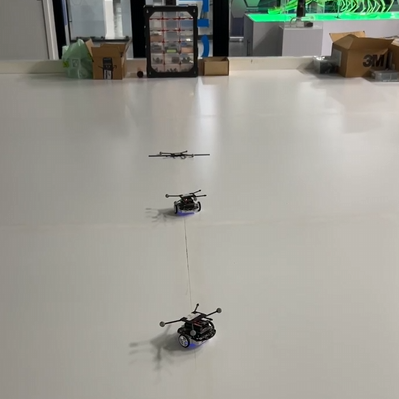
\includegraphics[width=0.45\textwidth]{replicar_fisico_pruebas/agente_inmovil_p1.png}
	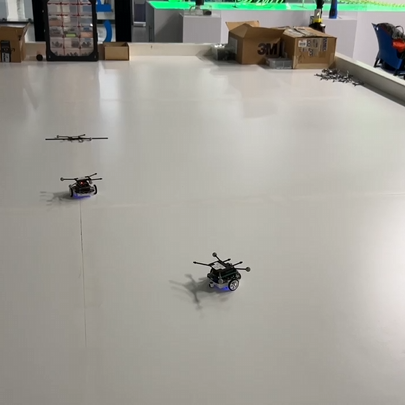
\includegraphics[width=0.45\textwidth]{replicar_fisico_pruebas/agente_inmovil_p2.png}
	\caption{Problema de funcionamiento en físico, agentes permanecen inmóviles.}
	\label{fig:agente_inmovil}
\end{figure}

Anteriormente, para obtener las poses de los marcadores se utilizaba una lista predeterminada con los valores enteros del $1$ al $12$ en orden ascendente que serían los marcadores a utilizar. Sin embargo esto ocasionaba diferentes problemas.

Para obtener las poses de los marcadores se utiliza la función ``robotat\_get\_pose'', esta recibe como argumentos el objeto TCP y los números de marcadores. Al tener una lista predeterminada de valores, siempre se está solicitando la pose de los $12$ marcadores aunque no todos estén en uso, resultando en una solicitud de datos innecesaria para el servidor. Además, dado que actualmente no se tienen disponibles los marcadores $1$ y $9$, se excede el tiempo de espera (\textit{Time Out}) para obtención de la pose de estos, lo que resulta en tiempos muertos durante la ejecución del código.

Para solucionar el problema, se optó por solicitar únicamente las poses de los marcadores a utilizar con una lista que contiene los números de todos los marcadores con el orden: agentes, objetivo y obstáculos. A continuación se muestra un ejemplo de esto.

Marcadores de agentes $= [1, 2, 3, 4]$

Marcador del objetivo $ = [22]$

Marcadores de obstáculos = $ = [14, 15, 16]$

Marcadores a solicitar $ = [1, 2, 3, 4, 22, 14, 15, 16]$


Por otro lado, para asignar los marcadores de cada agente, se debía elegir un intervalo  de valores consecutivos de manera ascendente dentro de la lista predeterminada. Esto era problemático ya que limita a utilizar únicamente los agentes dentro del intervalo seleccionado, por lo que si un agente se descargaba, era obligatorio reemplazar las baterías para volver a utilizarlo. Por esto, se optó por cambiar la asignación de los marcadores para cada agente permitiendo seleccionar cualquier marcador disponible en el Robotat sin algún orden específico y ahora, para obtener las poses de los marcadores, únicamente se solicitan los datos al servidor de los marcadores en uso. Esto además, permite agilizar las pruebas a realizar ya que en múltiples ocasiones es necesario compartir los agentes Pololu 3Pi+ con otros compañeros.

En la Figura \ref{fig:seleccion_agentes}, el número dentro del círculo, representa el número de marcador asignado al agente. A la izquierda se puede observar la asignación de los marcadores a cada agente con la implementación del algoritmo original, mientras del lado derecho se observa una asignación arbitraria luego del cambio mencionado.


\begin{figure}[H]
	\centering
	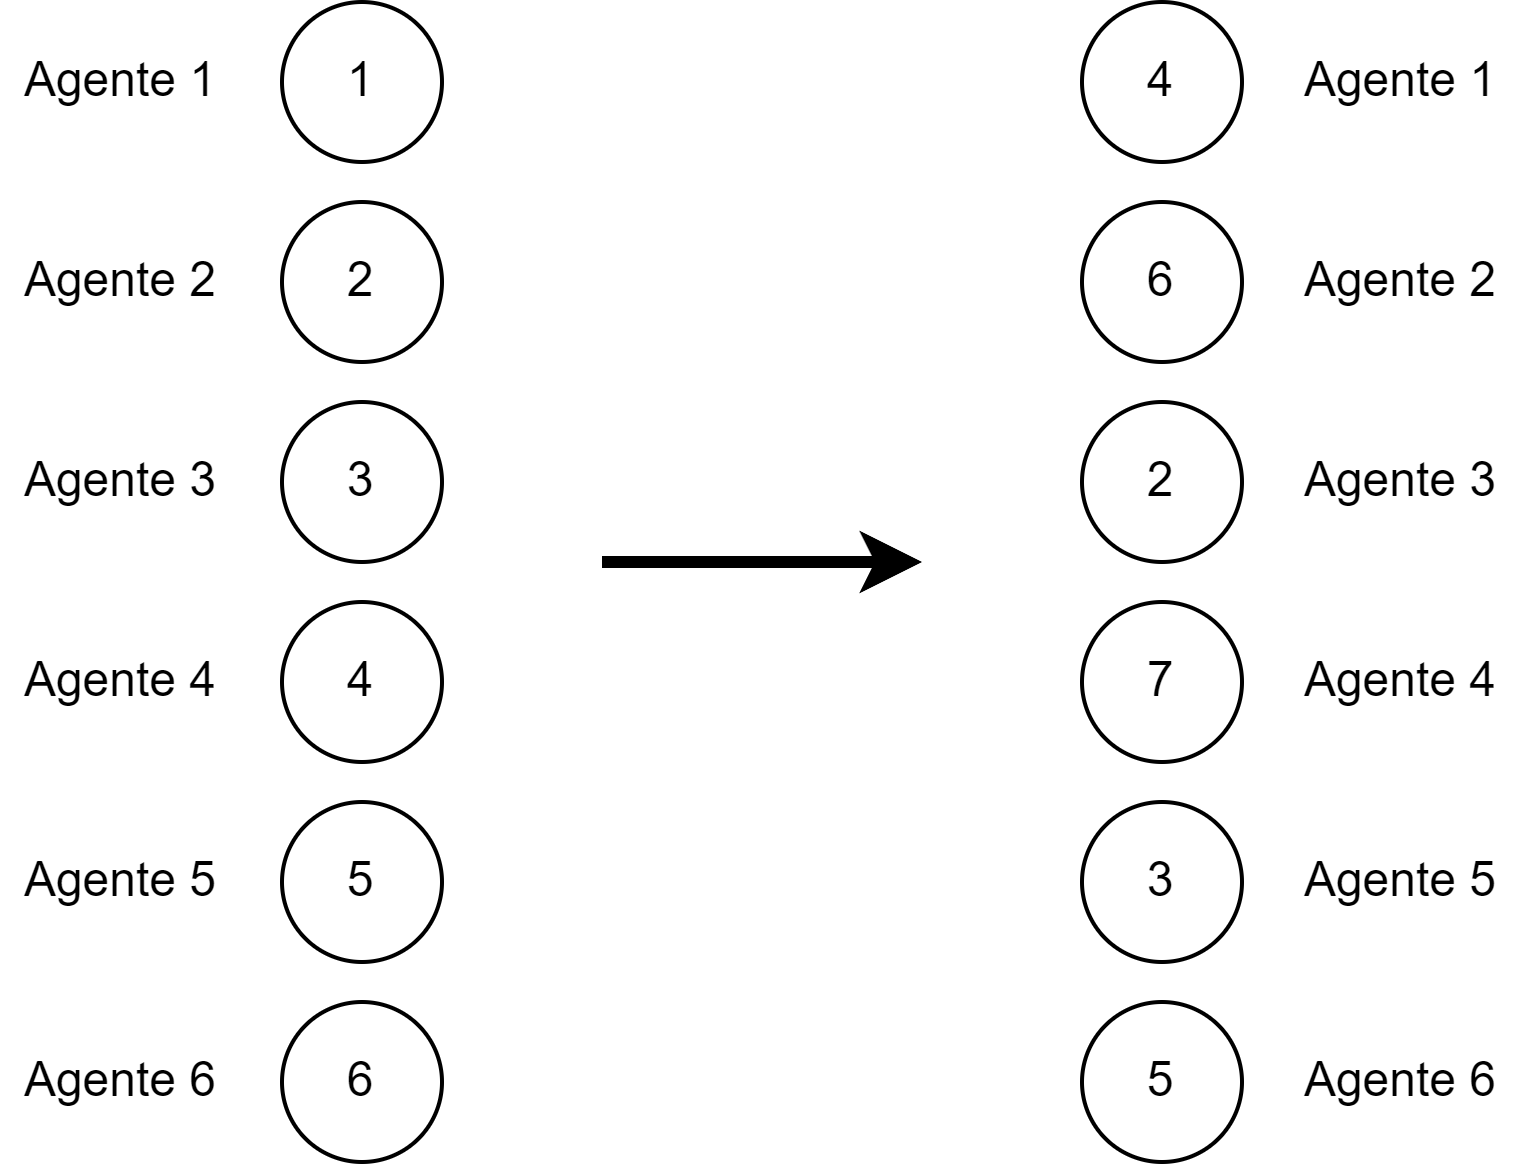
\includegraphics[width=0.6\textwidth]{replicar_fisico_pruebas/seleccion_agentes.png}
	\caption{Selección de marcadores para cada agente antes y después de las modificaciones.}
	\label{fig:seleccion_agentes}
\end{figure}


\subsection{Ajuste de parámetros en el algoritmo}
Una vez realizadas las modificaciones anteriores, al ejecutar el algoritmo en físico con tres agentes se encontró que su comportamiento es divergente en la etapa donde se movilizan hacia sus posiciones iniciales. En la Figura \ref{fig:divergencia1} se observa la trayectoria que toman los agentes.

\begin{figure}[H]
	\centering
	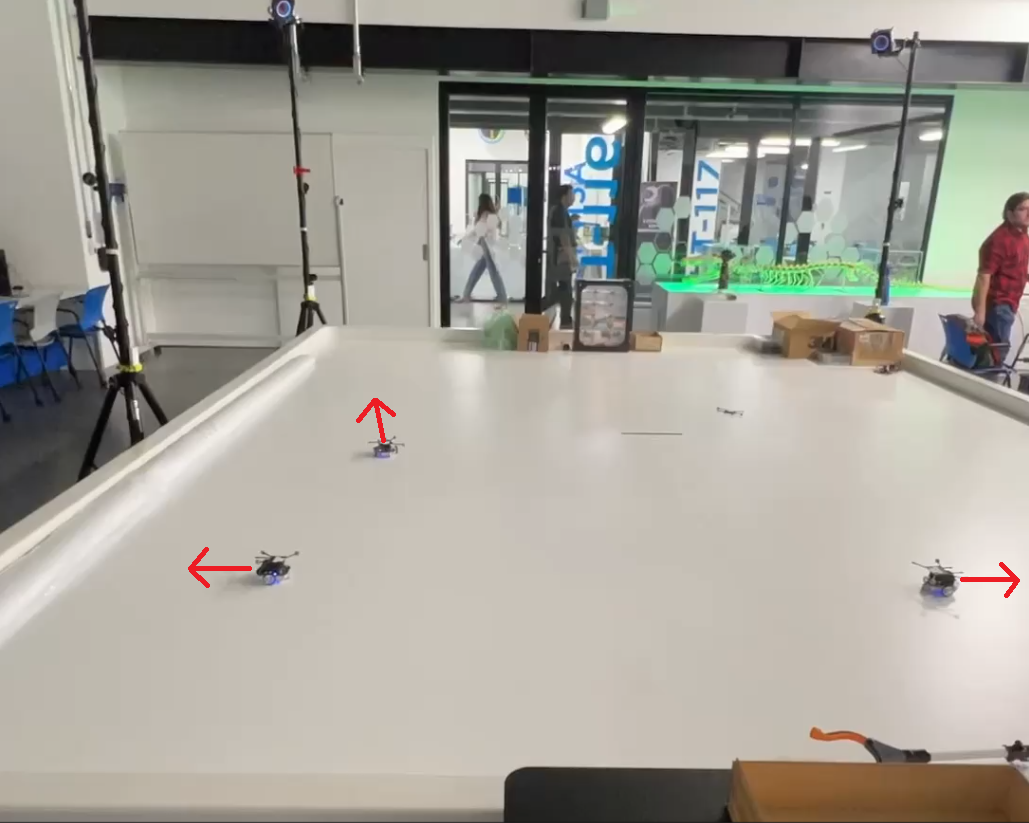
\includegraphics[width=0.45\textwidth]{replicar_fisico_pruebas/divergencia_p1.png}
	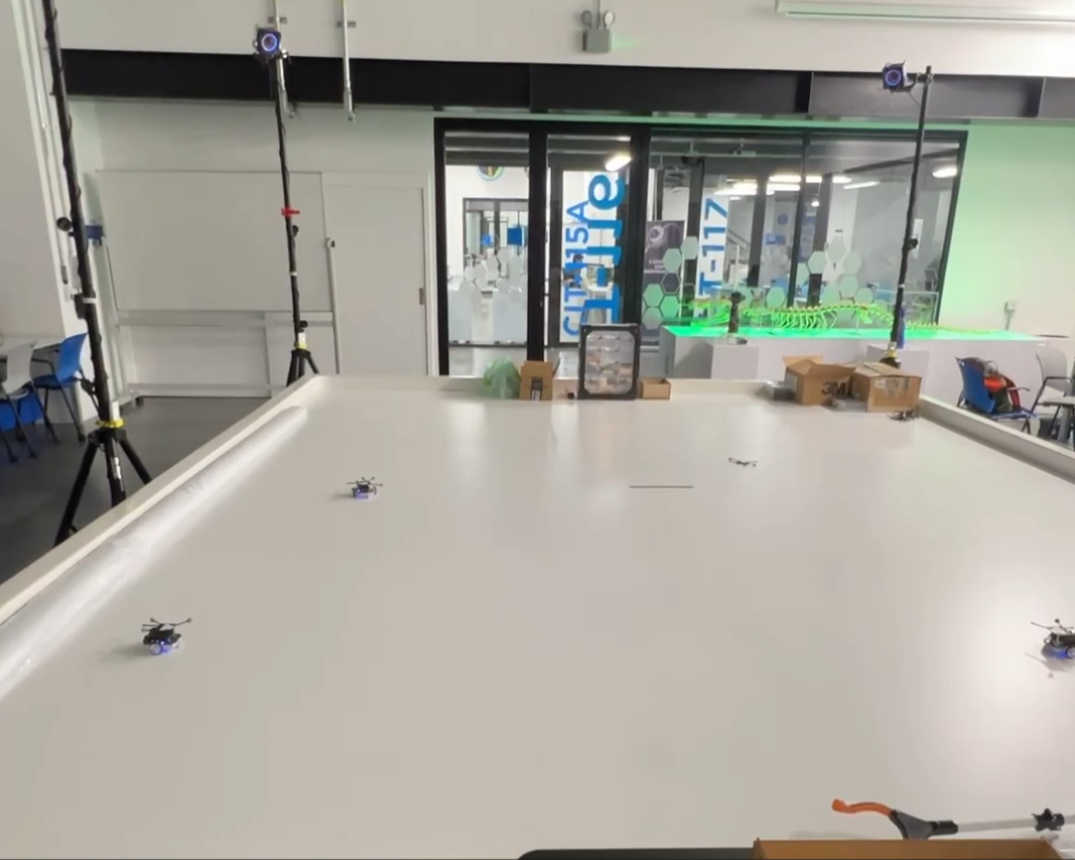
\includegraphics[width=0.45\textwidth]{replicar_fisico_pruebas/divergencia_p2.png}
	\caption{Problema de funcionamiento en físico, agentes divergen hacia posiciones iniciales. }
	\label{fig:divergencia1}
\end{figure}

Para intentar solucionar esto, se invirtió signo de la constante de proporcionalidad en el control de velocidad aplicado en la etapa 0 del algoritmo. Anteriormente se utilizaba $k = 5$, ahora se utiliza $k = -5$. Al aplicar el cambio, se encontró que ahora los agentes si se colocan en sus posiciones iniciales, sin embargo, ahora el comportamiento de divergencia se sigue presentando en las demás etapas del algoritmo tal como se observa en la Figura \ref{fig:divergencia2}.

\begin{figure}[H]
	\centering
	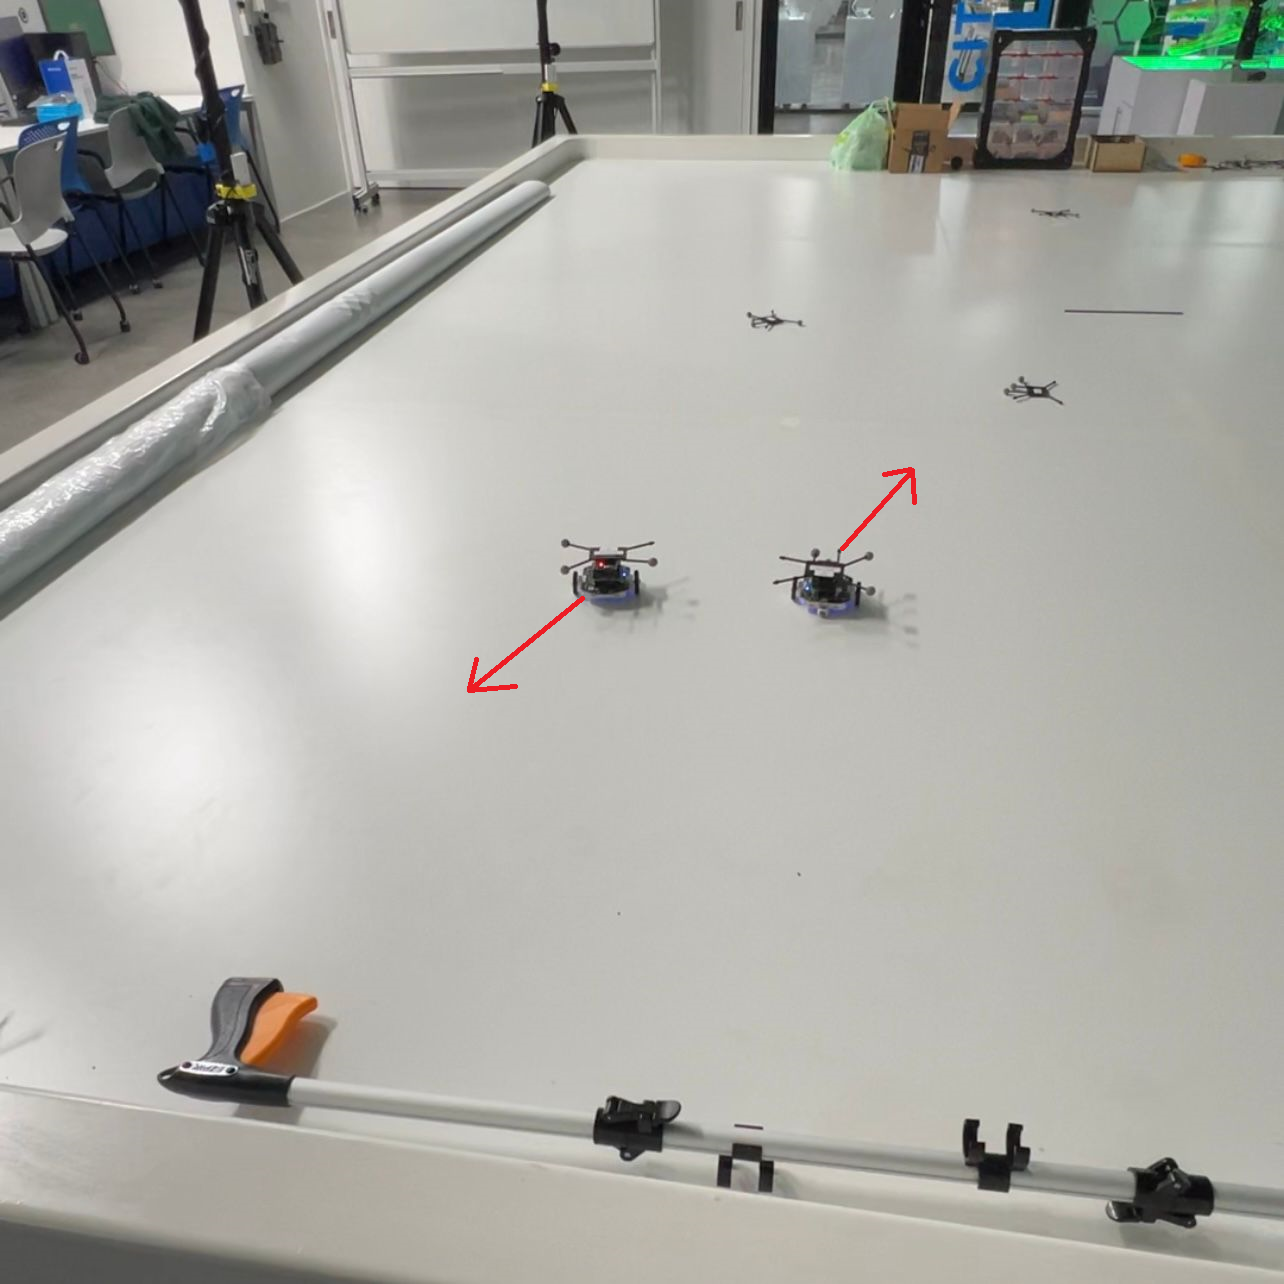
\includegraphics[width=0.45\textwidth]{replicar_fisico_pruebas/divergencia2_p1.png}
	\includegraphics[width=0.45\textwidth]{replicar_fisico_pruebas/divergencia2_p2.png}
	\caption{Problema de funcionamiento en físico, agentes divergen luego de colocarse en sus posiciones iniciales.}
	\label{fig:divergencia2}
\end{figure}

Al observar esto, se encontró que el patrón de divergencia se presentaba en todas las secciones donde se aplica el control proporcional para la velocidad de los agentes. Sabiendo esto, se optó por invertir el signo de la velocidad $v_n$ y la constante $k$ de la Ecuación (\ref{eq:controlador_proporcional}) tal como se observa a continuación:

\begin{equation}
	v_{n+1} = -v_n - k(x_{objetivo} - x_{agente})
	\label{eq:controlador_proporcional2}
\end{equation}

Con esto, se logró solucionar la divergencia de los agentes y se realizó la primera ejecución del algoritmo exitosa utilizando dos agentes, sin obstáculos tal como se observa en la Figura \ref{fig:prueba_fisico1}. Las imágenes en el orden de izquierda a derecha y luego de arriba hacia abajo muestran la secuencia de ejecución del algoritmo.

\begin{figure}[H]
	\centering
	\includegraphics[width=0.45\textwidth]{replicar_fisico_pruebas/prueba_fisico_p1.png}
	\includegraphics[width=0.45\textwidth]{replicar_fisico_pruebas/prueba_fisico_p2.png}
	\includegraphics[width=0.45\textwidth]{replicar_fisico_pruebas/prueba_fisico_p3.png}
	\includegraphics[width=0.45\textwidth]{replicar_fisico_pruebas/prueba_fisico_p4.png}
	\caption{Primera prueba exitosa de funcionamiento en físico.}
	\label{fig:prueba_fisico1}
\end{figure}

Una vez realizada la primera prueba, se simuló un escenario arbitrario en Webots, sin embargo se encontró que ahora la simulación presentaba los mismos patrones de divergencia en todas las etapas del algoritmo. Por esto, se optó por implementar el control proporcional de la Ecuación (\ref{eq:controlador_proporcional}) para las simulaciones y otro control proporcional con la Ecuación (\ref{eq:controlador_proporcional2}) para ejecutar el algoritmo en físico. Con esta modificación, se logró replicar el funcionamiento completo del algoritmo tanto para simulaciones en Webots como en un ambiente físico en el Robotat.

\subsection{Configuraciones para el escenario}
Para clasificar las ejecuciones del algoritmo según las condiciones del escenario, se decidió utilizar la misma convención implementada por José Alejandro Rodríguez \cite{RodriguezJA_2023_tesis}. Esta se enfoca en diferenciar los escenarios según las posiciones de las marcas iniciales para los agentes, los obstáculos y el objetivo.

En el Cuadro \ref{cuadro:configuraciones_escenario} se muestra la codificación a utilizar para los experimentos. El orden para identificarlos es el siguiente: (Posición inicial de los agentes)-(Obstáculos)-(Objetivo). A continuación, se presenta el ejemplo de clasificación A-D-B, que significa:

\begin{itemize}
	\item Posicionamiento inicial de los agentes en línea.
	\item Obstáculos móviles.
	\item Objetivo en el centro de la mesa de pruebas.
\end{itemize}

\begin{table}[H]
	\centering
	\resizebox{\textwidth}{!} {
		\begin{tabular}{|l|l|l|l|}
			\hline
			\textbf{Letra de designación} & \textbf{Posición inicial de los agentes} & \textbf{Obstáculos}                                                         & \textbf{Objetivo} \\ \hline
			A                              & Línea                                    & Ninguno                                                                     & Esquina           \\ \hline
			B                              & Círculo                                  & \begin{tabular}[c]{@{}l@{}}1 = Centro\\ 2 = Cerca del objetivo\end{tabular} & Centro            \\ \hline
			C                              & Aleatorio                                & Aleatorio                                                                   & Aleatorio         \\ \hline
			D                              & N/A                                      & Móviles                                                                     & Móvil             \\ \hline
	\end{tabular}}
	\caption{Configuraciones para el escenario.}
	\label{cuadro:configuraciones_escenario}
\end{table}

\subsection{Prueba del algoritmo en físico con escenarios previos}
Una vez solucionados los problemas anteriores, se realizó las primeras pruebas para replicar algunos de los escenarios físicos realizados por José Alejandro Rodríguez \cite{RodriguezJA_2023_tesis} y comprobar el funcionamiento correcto del algoritmo.

El código del supervisor ya cuenta con un sistema de guardado de información. Este almacena en un archivo .npz todos los datos relevantes al final del experimento. Además, con el archivo ``data\_graphing.py'' se generan las gráficas y trayectorias luego de que los agentes se hayan colocado en sus posiciones iniciales.

A continuación, se muestran algunos de los datos almacenados más relevantes:

\begin{itemize}
	\item Historial durante todo el experimento de:
	\begin{itemize}
		\item Posiciones y orientaciones de los agentes
		\item Posiciones de los obstáculos
		\item Posición del objetivo
		\item Velocidades de los agentes
	\end{itemize}
	\item Datos y configuraciones de:
	\begin{itemize}
		\item Ciclos del experimento
		\item Ciclo en que se logra el objetivo
		\item Ciclo en que inicia la etapa 1 del algoritmo
		\item Cantidad de agentes y sus números de marcadores asignados
		\item Cantidad de obstáculos y sus números de marcadores asignados
		\item Marcas de posiciones iniciales de los agentes
		\item Paso de tiempo del programa
	\end{itemize}
\end{itemize}

\subsubsection{Primer escenario}
Para el primer escenario, se utilizó la configuración AAA con 2 agentes. En las Figuras \ref{fig:test_fisico1} y \ref{fig:traj_test_2A_AAA_f_1} se muestra el escenario en la mesa de pruebas y las trayectorias de los agentes durante el experimento.

\begin{figure}[H]
	\centering
	\includegraphics[width=0.8\textwidth]{replicar_fisico_escenarios/test_f1.png}
	\caption{Mesa de pruebas con 2 agentes en el escenario AAA, corrida 1, en físico.}
	\label{fig:test_fisico1}
\end{figure}
\begin{figure}[H]
	\centering
	\includegraphics[width=0.8\textwidth]{replicar_fisico_escenarios/traj_test_2A_AAA_f_1.eps}
	\caption{Trayectoria de los 2 agentes en el escenario AAA, corrida 1, en físico.}
	\label{fig:traj_test_2A_AAA_f_1}
\end{figure}

\subsubsection{Segundo escenario}
Para el segundo escenario, se utilizó la configuración AAA con 6 agentes. En las Figuras \ref{fig:test_fisico2} y \ref{fig:traj_test_6A_AAA_f_1} se muestra el escenario en la mesa de pruebas y las trayectorias de los agentes durante el experimento.

\begin{figure}[H]
	\centering
	\includegraphics[width=0.8\textwidth]{replicar_fisico_escenarios/test_f2.png}
	\caption{Mesa de pruebas con 6 agentes en el escenario AAA, corrida 1, en físico.}
	\label{fig:test_fisico2}
\end{figure}
\begin{figure}[H]
	\centering
	\includegraphics[width=0.8\textwidth]{replicar_fisico_escenarios/traj_test_6A_AAA_f_1.eps}
	\caption{Trayectoria de los 6 agentes en el escenario AAA, corrida 1, en físico.}
	\label{fig:traj_test_6A_AAA_f_1}
\end{figure}

\subsubsection{Tercer escenario}
Para el tercer escenario, se utilizó la configuración ACA con 6 agentes. En las Figuras \ref{fig:test_fisico3} y \ref{fig:traj_test_6A_ACA_f_1} se muestra el escenario en la mesa de pruebas y las trayectorias de los agentes durante el experimento.

\begin{figure}[H]
	\centering
	\includegraphics[width=0.8\textwidth]{replicar_fisico_escenarios/test_f3.png}
	\caption{Mesa de pruebas con 6 agentes en el escenario ACA, corrida 1, en físico.}
	\label{fig:test_fisico3}
\end{figure}
\begin{figure}[H]
	\centering
	\includegraphics[width=0.8\textwidth]{replicar_fisico_escenarios/traj_test_6A_ACA_f_1.eps}
	\caption{Trayectoria de los 6 agentes en el escenario ACA, corrida 1, en físico.}
	\label{fig:traj_test_6A_ACA_f_1}
\end{figure}

\subsubsection{Cuarto escenario}
Para el tercer escenario, se utilizó la configuración ACC con 3 agentes. En las Figuras \ref{fig:test_fisico4} y \ref{fig:traj_test_3A_ACC_f_1} se muestra el escenario en la mesa de pruebas y las trayectorias de los agentes durante el experimento.

\begin{figure}[H]
	\centering
	\includegraphics[width=0.8\textwidth]{replicar_fisico_escenarios/test_f4.png}
	\caption{Mesa de pruebas con 3 agentes en el escenario ACC, corrida 1, en físico.}
	\label{fig:test_fisico4}
\end{figure}
\begin{figure}[H]
	\centering
	\includegraphics[width=0.8\textwidth]{replicar_fisico_escenarios/traj_test_3A_ACC_f_1.eps}
	\caption{Trayectoria de los 3 agentes en el escenario ACC, corrida 1, en físico.}
	\label{fig:traj_test_3A_ACC_f_1}
\end{figure}

\subsubsection{Quinto escenario}
Para el tercer escenario, se utilizó la configuración ACA con 3 agentes. En las Figuras \ref{fig:test_fisico5} y \ref{fig:traj_test_3A_ACA_f_1} se muestra el escenario en la mesa de pruebas y las trayectorias de los agentes durante el experimento.

\begin{figure}[H]
	\centering
	\includegraphics[width=0.8\textwidth]{replicar_fisico_escenarios/test_f5.png}
	\caption{Mesa de pruebas con 3 agentes en el escenario ACA, corrida 1, en físico.}
	\label{fig:test_fisico5}
\end{figure}
\begin{figure}[H]
	\centering
	\includegraphics[width=0.8\textwidth]{replicar_fisico_escenarios/traj_test_3A_ACA_f_1.eps}
	\caption{Trayectoria de los 3 agentes en el escenario ACA, corrida 1, en físico.}
	\label{fig:traj_test_3A_ACA_f_1}
\end{figure}

\section{Prueba de funcionamiento del algoritmo con obstáculos móviles}
Una vez que se validó el funcionamiento del algoritmo utilizando escenarios previos, se puso a prueba la naturaleza dinámica del algoritmo de sincronización y control de formaciones. Como se mencionó anteriormente, se cuenta con el archivo ``data\_graphing.py'' para generar las gráficas y trayectorias del experimento. Sin embargo, este no muestra el recorrido de los obstáculos en movimiento, por lo que se agregó esta función a manera de visualizar la posición inicial, y final, así como las trayectorias de los obstáculos.

A continuación, se presentan los escenarios en los que se puso a prueba el algoritmo con obstáculos móviles en simulaciones y en físico. En todos los casos, se observa que los agentes logran reposicionarse y cambiar su trayectoria al moverse los obstáculos, manteniendo su formación mientras siguen el objetivo. Esto es posible gracias a la naturaleza dinámica del algoritmo, que se debe a la manera en que se planteó originalmente la ecuación de consenso y el cálculo del peso para determinar las velocidades. Además, el algoritmo está constantemente evaluando la posición actual de cada agente y la compara con la posición actual de los obstáculos. Con esto, se ajusta de forma dinámica el peso $w$ y se re calcula la ecuación de consenso para evitar posibles colisiones.

\subsection{Simulaciones utilizando obstáculos móviles}
Para las simulaciones mostradas en las Figuras \ref{fig:traj_testSim_6A_ADA_v_1}, \ref{fig:traj_testSim_6A_ADA_v_2} y \ref{fig:traj_testSim_6A_ADA_v_3} se optó por utilizar una configuración ADA con 6 agentes y se movilizó los obstáculos a manera de que estos interfirieran con la trayectoria de la formación durante el seguimiento al objetivo. Cabe mencionar que la movilización de los obstáculos se hizo de manera aleatoria y sin ningún patrón en específico. 

\subsubsection{Primer escenario}
\begin{figure}[H]
	\centering
	\includegraphics[width=0.8\textwidth]{test_sim_ObsM/traj_testSim_6A_ADA_v_1.eps}
	\caption{Trayectoria de los 6 agentes en el escenario ADA, corrida 1, en simulación.}
	\label{fig:traj_testSim_6A_ADA_v_1}
\end{figure}

\subsubsection{Segundo escenario}
\begin{figure}[H]
	\centering
	\includegraphics[width=0.8\textwidth]{test_sim_ObsM/traj_testSim_6A_ADA_v_2.eps}
	\caption{Trayectoria de los 6 agentes en el escenario ADA, corrida 2, en simulación.}
	\label{fig:traj_testSim_6A_ADA_v_2}
\end{figure}

\subsubsection{Tercer escenario}
\begin{figure}[H]
	\centering
	\includegraphics[width=0.8\textwidth]{test_sim_ObsM/traj_testSim_6A_ADA_v_3.eps}
	\caption{Trayectoria de los 6 agentes en el escenario ADA, corrida 3, en simulación.}
	\label{fig:traj_testSim_6A_ADA_v_3}
\end{figure}


\subsection{Escenarios físicos utilizando obstáculos móviles}
A diferencia que con los escenarios en simulaciones, para las pruebas en físico se movilizó los obstáculos a manera de que estos interfirieran o liberaran una trayectoria de la formación durante el seguimiento al objetivo.

\subsubsection{Primer escenario}
Para este escenario, se movilizaron los obstáculos para que estos dejaran libre la trayectoria de los agentes hacia el objetivo en lugar de interferir en esta. Como se observa en la Figura \ref{fig:traj_test_3A_ADB_f_1}, el agente 1 con la trayectoria roja, pasa sobre la posición donde se encontraba el obstáculo inicialmente. Además, evita colisionar con los obstáculos colocados en sus posiciones finales. 

\begin{figure}[H]
	\centering
	\includegraphics[width=0.8\textwidth]{test_fisico_ObsM/traj_test_3A_ADB_f_1.eps}
	\caption{Trayectoria de los 3 agentes en el escenario ADB, corrida 1, en físico.}
	\label{fig:traj_test_3A_ADB_f_1}
\end{figure}

\subsubsection{Segundo escenario}
Para este escenario, se planteó el recorrido a manera que los agentes tuvieran que pasar en medio de los obstáculos. Como se observa en la Figura \ref{fig:traj_test_3A_ADC_f_1}, con la trayectoria en verde, el obstáculo se movilizó a lo largo del espacio libre para que este bloqueara el camino hacia el objetivo. Luego se volvió a colocar cercano a su posición inicial. Además, se observa cómo los agentes lograron evitar la colisión y seguir su trayecto una vez que el camino se liberara.
\begin{figure}[H]
	\centering
	\includegraphics[width=0.8\textwidth]{test_fisico_ObsM/traj_test_3A_ADC_f_1.eps}
	\caption{Trayectoria de los 3 agentes en el escenario ADC, corrida 1, en físico.}
	\label{fig:traj_test_3A_ADC_f_1}
\end{figure}

\subsubsection{Tercer escenario}
Para este caso, se realizó lo mismo que en el segundo escenario. Como se observa en la Figura \ref{fig:traj_test_3A_ADC_f_3}, con la trayectoria en verde, el obstáculo se movilizó a lo largo del espacio libre a manera que este bloqueara el camino hacia el objetivo. Luego se volvió a colocar cercano a su posición inicial, donde se observa cómo los agentes lograron evitar la colisión y seguir su trayecto una vez que el camino se liberara.

\begin{figure}[H]
	\centering
	\includegraphics[width=0.8\textwidth]{test_fisico_ObsM/traj_test_3A_ADC_f_3.eps}
	\caption{Trayectoria de los 3 agentes en el escenario ADC, corrida 3, en físico.}
	\label{fig:traj_test_3A_ADC_f_3}
\end{figure}

\subsubsection{Cuarto escenario}
Para este escenario, se movilizó el obstáculo una sola vez a manera que cambiara de posición e interfiriera con una trayectoria en línea recta de la formación hacia el objetivo. En la Figura \ref{fig:traj_test_3A_ADC_f_2}, se observa que los agentes modificaron su trayectoria evadiendo el obstáculo por un costado y siguieron exitosamente su camino hacia el objetivo.

\begin{figure}[H]
	\centering
	\includegraphics[width=0.8\textwidth]{test_fisico_ObsM/traj_test_3A_ADC_f_2.eps}
	\caption{Trayectoria de los 3 agentes en el escenario ADC, corrida 2, en físico.}
	\label{fig:traj_test_3A_ADC_f_2}
\end{figure}


\chapter{Optimización del algoritmo y su implementación}
En este capítulo se describen los puntos de mejora identificados en la implementación del algoritmo de sincronización y control de formaciones. Luego, se detallará cómo se abordó cada uno de ellos empleando técnicas de optimización como la reducción de complejidad computacional y ajuste de parámetros de control.

\section{Lenguaje de programación y limpieza de código}
El primer paso para la optimización fue analizar el lenguaje de programación empleado para los controladores. Se tomó en cuenta tres lenguajes para compararlos en base a las ventajas y desventajas que proponen para su implementación con el estado actual del algoritmo: MATLAB, Python y C. En el Cuadro \ref{cuadro:lenguajes_programacion} se describen las ventajas y desventajas que tiene un lenguaje sobre otro.

\begin{table}[H]
	\centering
	\resizebox{\textwidth}{!} {
	\begin{tabular}{|l|l|l|}
		\hline
		Lenguaje & Ventajas                                                                                                                                                                                                                                                                                                     & Desventajas                                                                                                                                                                                                                                                                                                             \\ \hline
		MATLAB   & \begin{tabular}[c]{@{}l@{}}- Es fácil de usar para simulaciones y prototipos.\\ \\ - Tiene una amplia variedad de herramientas \\ matemáticas.\\ \\ - Es excelente para algoritmos que involucran \\ operaciones matriciales.\end{tabular}                                                                      & \begin{tabular}[c]{@{}l@{}}- Es un lenguaje propio de MATLAB por lo que requiere comprar \\ licencias de software.\\ \\ - Su eficiencia computacional es menor en cuanto a rendimiento \\ comparado con Python o C.\end{tabular}                                                                                          \\ \hline
		Python   & \begin{tabular}[c]{@{}l@{}}- Es un lenguaje de código abierto (\textit{open source}).\\ \\ - Tiene una amplia variedad de librerías para optimizar \\ el cálculo numérico como NumPy, SciPy, multithreading \\ o multiprocessing.\\ \\ - Tiene un buen equilibrio entre rendmiento \\ computacional y facilidad de desarrollo.\end{tabular} & \begin{tabular}[c]{@{}l@{}}- Es un lenguaje más eficiente que MATLAB pero menos eficiente \\ que C debido a que es un lenguaje interpretado.\\ \\ - Requiere dependencias externas para lograr un alto rendimiento \\ (como integraciones con C).\end{tabular}                                                            \\ \hline
		C        & \begin{tabular}[c]{@{}l@{}}- Tiene un rendimiento superior ya que es un lenguaje \\ compilado de bajo nivel.\\ \\ - Ofrece un control sobre la memoria y el hardware.\end{tabular}                                                                                                                             & \begin{tabular}[c]{@{}l@{}}- Su complejidad es mucho mayor en cuando a implementación y \\ mantenimiento.\\ \\ - Tiene una alta probabilidad de fugas de memoria. \\ \\ - Requiere mucho más tiempo de desarrollo y es menos intuitivo.\\ \\ - No es tan flexible para realizar cambios rápidos en algoritmos.\end{tabular} \\ \hline
	\end{tabular}}
	\caption{Ventajas y desventajas de lenguajes de programación.}
	\label{cuadro:lenguajes_programacion}
\end{table}

Una vez comparados los lenguajes de programación se optó por seguir utilizando Python para el desarrollo de los controladores. Las razones principales fueron que es un lenguaje de código abierto y ofrece un buen equilibrio entre rendimiento computacional y facilidad de desarrollo. Además, ya se cuenta con todo el algoritmo previo desarrollado en Python funcionando en un entorno físico como el Robotat. Esto incluye el desarrollo de los controladores, funciones para cálculos propios del algoritmo de sincronización y control de formaciones y funciones de conexión con el servidor del Robotat y los Pololu 3Pi+. Por lo que, dado el poco tiempo disponible para utilizar el Robotat no es conveniente migrar a un nuevo lenguaje de programación para esta fase de la implementación del algoritmo. Además, python cuenta con librerías como NumPy que está basada en C y otras librerías de comunicación y procesamiento que permiten optimizar el rendimiento computacional.

Finalmente, se realizó un proceso de limpieza y documentación del código para facilitar las iteraciones a realizar. Además, esto permitió eliminar segmentos de código obsoletos, así como identificar otras deficiencias que se mencionarán a continuación.

\section{Posición de cada agente según el grafo de formación}
Durante la restauración del algoritmo desarrollado en fases previas, al implementar la selección manual de marcadores para los agentes, se encontró que anteriormente el número de marcador asignado a cada agente estaba directamente relacionado con la posición que este debe tomar según el grafo de formación. En la Figura \ref{fig:grafo_formacion1} se muestra la asignación de posiciones según el grafo de formación para una selección arbitraria de agentes con la implementación original del algoritmo.

\begin{figure}[H]
	\centering
	\includegraphics[width=0.8\textwidth]{optimizacion/grafo_formacion1.png}
	\caption{Posiciones de agentes según el grafo de formación con la implementación original del algoritmo.}
	\label{fig:grafo_formacion1}
\end{figure}

Al tener una formación como la mostrada anteriormente se vuelve poco intuitiva su visualización a la hora de ejecutar el algoritmo. Por esto, se decidió cambiar la asignación de posición de cada agente a manera que siempre se mantenga la misma estructura del grafo de formación y los agentes se posicionen de manera ascendente tal como se observa en la figura \ref{fig:grafo_formacion2}.

\begin{figure}[H]
	\centering
	\includegraphics[width=0.8\textwidth]{optimizacion/grafo_formacion2.png}
	\caption{Posiciones de agentes según el grafo de formación con la implementación original del algoritmo.}
	\label{fig:grafo_formacion2}
\end{figure}
	
\section{Mejorar la eficiencia computacional con NumPy}
NumPy es una librería de Python especializada para el cálculo numérico y científico. Destaca por su soporte para trabajar con operaciones vectorizadas o vectores multidimensionales sin realizar bucles. También cuenta con una amplia variedad de funciones matemáticas y estadísticas, así como integración con otras bibliotecas como SciPy. Además, NumPy está implementado en C por lo que permite mejorar la eficiencia computacional para grandes cantidades de datos.

Al revisar los programas de los controladores, se encontró varios segmentos de código que se realizan con ciclos \textit{for} simples y otros anidados. Esto presenta una deficiencia al realizar los cálculos y solicitud de datos al servidor del Robotat por lo que se optó por optimizar dichos procesos utilizando funciones matemáticas y operaciones matriciales con NumPy. A continuación, se detallará los segmentos del algoritmo que se optimizaron implementando operaciones con NumPy y se mostrará la comparativa en cuanto a tiempos de ejecución utilizando la librería ``time'' de Python y análisis estadísticos.

\subsection{Aplicar desfases de los marcadores}
A continuación se explica los pasos que se realizaban anteriormente para aplicar los desfases de la calibración de marcadores, donde $n$ es la cantidad de marcadores a utilizar.

\begin{itemize}
	\item Configuración
	\begin{enumerate}
		\item Cargar el archivo .npy con los desfases de los marcadores.
		\item Solicitar las poses de $n$ marcadores al sevidor del Robotat.
		\item Aplicar el desfase de cada marcador con un ciclo \textit{for} de $n$ iteraciones.
	\end{enumerate}
	\item Ciclo principal 
	\begin{enumerate}
		\item Solicitar las poses de $n$ marcadores al servidor del Robotat.
		\item Aplicar el desfase de cada marcador con un ciclo \textit{for} de $n$ iteraciones.
	\end{enumerate}
\end{itemize}

Sin embargo, el implementar ciclos \textit{for} dentro del ciclo principal significa un aumento de tiempo computacional que es más notorio al aumentar la cantidad de marcadores a utilizar. Para optimizar el proceso se optó por aplicar los desfases a cada marcador utilizando operaciones matriciales e implementando únicamente una resta de matrices dentro del ciclo principal, por lo que ahora el proceso es el siguiente:

\begin{itemize}
	\item Configuración
	\begin{enumerate}
		\item Cargar el archivo .npy con los desfases de los marcadores.
		\item Almacenar los desfases en la cuarta columna de una matriz de ceros de tamaño $n \times 6$.
		\item Solicitar las poses de los marcadores al sevidor del Robotat.
		\item Aplicar el desfase de los marcadores con una resta de la matriz con los desfases a la matriz con las poses de los marcadores.
	\end{enumerate}
	\item Ciclo principal 
	\begin{enumerate}
		\item Solicitar las poses de los marcadores al servidor del Robotat
		\item Aplicar el desfase de los marcadores con una resta de la matriz con los desfases a la matriz con las poses de los marcadores.
	\end{enumerate}
\end{itemize}

Una vez implementada la optimización, se realizó un análisis estadístico con mil muestras donde se tomó el tiempo que toma aplicar los desfases a los marcadores con un ciclo \textit{for} y con una resta de matrices con NumPy.

Para la toma de muestras, se evaluó diferentes cantidades de marcadores a los que se les aplicaría el desfase, siendo estos 5, 10, 15 y 20. En los Cuadros \ref{cuadro:tiempos_desfases_for} y \ref{cuadro:tiempos_desfases_numpy} se muestra la media y desviación estándar del tiempo que toma aplicar los desfases.

En la Figura \ref{fig:grafica_tiempos_desfases} se observa que la optimización con NumPy presenta una reducción notable en el tiempo de procesamiento, la cual es aún más significativa a medida que aumenta la cantidad de marcadores a utilizar. Por otro lado, los tiempos al aplicar ciclos \textit{for} incrementan de manera proporcional y más pronunciada con el aumento de los marcadores, mientras que con NumPy el crecimiento es más moderado ya que la pendiente de la curva es dos órdenes de magnitud menor.

\begin{table}[H]
	\centering
	\resizebox{\textwidth}{!} {
	\begin{tabular}{|l|l|l|l|}
		\hline
		\textbf{Cantidad de marcadores} & \textbf{Número de muestras} & \textbf{Media de tiempo (ms)} & \textbf{Desviación estándar (ms)} \\ \hline
		5 & 1000 & 0.002802 & 0.000308 \\ \hline
		10 & 1000 & 0.005353 & 0.000469 \\ \hline
		15 & 1000 & 0.008187 & 0.001654 \\ \hline
		20 & 1000 & 0.010485 & 0.000843 \\ \hline
	\end{tabular}}
	\caption{Media de tiempo y desviación estándar para aplicar desfases de marcadores con ciclos \text{for}.}
	\label{cuadro:tiempos_desfases_for}
\end{table}

\begin{table}[H]
	\centering
	\resizebox{\textwidth}{!} {
	\begin{tabular}{|l|l|l|l|}
		\hline
		\textbf{Cantidad de marcadores} & \textbf{Número de muestras} & \textbf{Media de tiempo (ms)} & \textbf{Desviación estándar (ms)} \\ \hline
		5 & 1000 & 0.000734 & 0.000119 \\ \hline
		10 & 1000 & 0.000756 & 0.000113 \\ \hline
		15 & 1000 & 0.000794 & 0.000225 \\ \hline
		20 & 1000 & 0.000837 & 0.000147 \\ \hline
	\end{tabular}}
	\caption{Media de tiempo y desviación estándar para aplicar desfases de marcadores con NumPy.}
	\label{cuadro:tiempos_desfases_numpy}
\end{table}

\begin{figure}[H]
	\centering
	\includegraphics[width=\textwidth]{optimizacion/tiempos_desfases.png}
	\caption{Gráfica con medias de tiempo para aplicar desfases de marcadores con ciclos \textit{for} y operaciones con NumPy.}
	\label{fig:grafica_tiempos_desfases}
\end{figure}

\subsection{Cálculo de la distancia entre agentes}
Para el cálculo de distancia entre agentes se tiene una función llamada ``DistBetweenAgents'' dentro del archivo ``funciones.py''. Esta utiliza dos ciclos \textit{for} anidados para calcular la norma de distancia basada en la distancia en $x$ y $y$ de cada agente hacia sus vecinos más próximos. El cálculo de la distancia se realiza entre los agentes $i$ y $j$ y luego para $j$ e $i$, esto produce una matriz simétrica por lo que se puede realizar únicamente el cálculo de una mitad y luego duplicarla. Para esto, se creó una versión optimizada de la función llamada ``DistBetweenAgentsOptimized''. En esta, únicamente se calcula la diferencia de posiciones aprovechando el \textit{broadcasting} en NumPy y luego se obtiene la norma de la matriz de distancias utilizando la función ``linealg.norm''.

En los Cuadros \ref{cuadro:tiempos_distancias_for} y \ref{cuadro:tiempos_distancias_numpy} se muestra la media y desviación estándar del tiempo que toma en realizar los cálculos con la función original y la optimizada. Para esto, se tomó mil muestras aumentando la cantidad de agentes desde $1$ hasta $10$. 

En la Figura \ref{fig:grafica_tiempos_distancias} se observa un incremento exponencial en el tiempo de procesamiento al calcular las distancias entre los agentes conforme se aumenta el número de estos en la formación. Además, la optimización con NumPy presenta un incremento significativamente menor. Esto se confirma al observar que el exponente de la ecuación que describe el comportamiento utilizando ciclos \textit{for} es $1.6982$, mientras que el exponente al utilizar NumPy es $0.1775$.

\begin{table}[H]
	\centering
	\resizebox{\textwidth}{!} {
	\begin{tabular}{|l|l|l|l|}
		\hline
		\textbf{Cantidad de marcadores} & \textbf{Número de muestras} & \textbf{Media de tiempo (ms)} & \textbf{Desviación estándar (ms)} \\ \hline
		1 & 1000 & 0.00213 & 0.000343 \\ \hline
		2 & 1000 & 0.005569 & 0.006185 \\ \hline
		3 & 1000 & 0.009883 & 0.000914 \\ \hline
		4 & 1000 & 0.016406 & 0.001267 \\ \hline
		5 & 1000 & 0.026257 & 0.005967 \\ \hline
		6 & 1000 & 0.036697 & 0.00706 \\ \hline
		7 & 1000 & 0.051342 & 0.003965 \\ \hline
		8 & 1000 & 0.062752 & 0.012055 \\ \hline
		9 & 1000 & 0.079696 & 0.009144 \\ \hline
		10 & 1000 & 0.098319 & 0.009456 \\ \hline
	\end{tabular}}
	\caption{Media de tiempo y desviación estándar para calcular la distancia entre agentes con ciclos \textit{for}.}
	\label{cuadro:tiempos_distancias_for}
\end{table}

\begin{table}[H]
	\centering
	\resizebox{\textwidth}{!} {
	\begin{tabular}{|l|l|l|l|}
		\hline
		\textbf{Cantidad de marcadores} & \textbf{Número de muestras} & \textbf{Media de tiempo (ms)} & \textbf{Desviación estándar (ms)} \\ \hline
		1 & 1000 & 0.0061 & 0.001477 \\ \hline
		2 & 1000 & 0.008134 & 0.001457 \\ \hline
		3 & 1000 & 0.008187 & 0.007005 \\ \hline
		4 & 1000 & 0.008354 & 0.006599 \\ \hline
		5 & 1000 & 0.008918 & 0.00158 \\ \hline
		6 & 1000 & 0.008835 & 0.001695 \\ \hline
		7 & 1000 & 0.009344 & 0.001726 \\ \hline
		8 & 1000 & 0.009559 & 0.004158 \\ \hline
		9 & 1000 & 0.009581 & 0.002898 \\ \hline
		10 & 1000 & 0.009614 & 0.002514 \\ \hline
	\end{tabular}}
	\caption{Media de tiempo y desviación estándar para calcular la distancia entre agentes con NumPy.}
	\label{cuadro:tiempos_distancias_numpy}
\end{table}

\begin{figure}[H]
	\centering
	\includegraphics[width=\textwidth]{optimizacion/tiempos_distancias.png}
	\caption{Gráfica con medias de tiempo para calcular la distancia entre agentes con ciclos \textit{for} y operaciones con NumPy.}
	\label{fig:grafica_tiempos_distancias}
\end{figure}

\subsection{Cálculo del error de formación}
Para calcular el error de formación se utiliza la función ``FormationError'' dentro del archivo ``funciones.py''. Esta función utiliza dos ciclos \textit{for} anidados para calcular el error cuadrático medio entre la formación actual y la deseada utilizando como parámetros las matrices de adyacencia de ambas formaciones. Dado que ambas matrices son cuadradas y, al considerar únicamente los agentes de interés, se convierten en matrices del mismo tamaño, se desarrolló una versión optimizada de la función llamada ``FormationErrorOptimized''. Esta versión emplea la función ``square'' de NumPy que eleva al cuadrado cada elemento de la matriz y luego calcula la media utilizando la función ``mean''.


En los Cuadros \ref{cuadro:tiempos_error_for} y \ref{cuadro:tiempos_error_numpy} se muestra la media y desviación estándar del tiempo que toma en realizar el cálculo del error cuadrático medio con la función original y la optimizada. Para esto, se tomó mil muestras aumentando la cantidad de agentes desde $1$ hasta $10$. 

En la Figura \ref{fig:grafica_tiempos_error} se muestra una gráfica en la que se evidencia un crecimiento exponencial en el tiempo de procesamiento al calcular las distancias entre los agentes a medida que se aumenta el número de agentes en la formación. Por otro lado, la optimización con Numpy, presenta un aumento significativamente menor. Además, esto se demuestra ya que el exponente de la ecuación que describe el comportamiento utilizando ciclos \textit{for} es $1.4753$, mientras que el exponente para la optimización con NumPy es $0.112$.

\begin{table}[H]
	\centering
	\resizebox{\textwidth}{!} {
	\begin{tabular}{|l|l|l|l|}
		\hline
		\textbf{Cantidad de marcadores} & \textbf{Número de muestras} & \textbf{Media de tiempo (ms)} & \textbf{Desviación estándar (ms)} \\ \hline
		1 & 1000 & 0.005665 & 0.000809 \\ \hline
		2 & 1000 & 0.01101 & 0.000895 \\ \hline
		3 & 1000 & 0.018721 & 0.008085 \\ \hline
		4 & 1000 & 0.029093 & 0.00714 \\ \hline
		5 & 1000 & 0.043071 & 0.003761 \\ \hline
		6 & 1000 & 0.058559 & 0.008292 \\ \hline
		7 & 1000 & 0.075147 & 0.010952 \\ \hline
		8 & 1000 & 0.103554 & 0.008648 \\ \hline
		9 & 1000 & 0.128032 & 0.011905 \\ \hline
		10 & 1000 & 0.149833 & 0.013256 \\ \hline
	\end{tabular}}
	\caption{Media de tiempo y desviación estándar para calcular el error de formación con ciclos \textit{for}.}
	\label{cuadro:tiempos_error_for}
\end{table}

\begin{table}[H]
	\centering
	\resizebox{\textwidth}{!} {
	\begin{tabular}{|l|l|l|l|}
		\hline
		\textbf{Cantidad de marcadores} & \textbf{Número de muestras} & \textbf{Media de tiempo (ms)} & \textbf{Desviación estándar (ms)} \\ \hline
		1 & 1000 & 0.016538 & 0.007916 \\ \hline
		2 & 1000 & 0.020229 & 0.002389 \\ \hline
		3 & 1000 & 0.020081 & 0.003186 \\ \hline
		4 & 1000 & 0.020134 & 0.003423 \\ \hline
		5 & 1000 & 0.020714 & 0.003501 \\ \hline
		6 & 1000 & 0.021065 & 0.00453 \\ \hline
		7 & 1000 & 0.021143 & 0.005589 \\ \hline
		8 & 1000 & 0.022082 & 0.003146 \\ \hline
		9 & 1000 & 0.022348 & 0.00473 \\ \hline
		10 & 1000 & 0.022455 & 0.024888 \\ \hline
	\end{tabular}}
	\caption{Media de tiempo y desviación estándar para calcular el error de formación con NumPy.}
	\label{cuadro:tiempos_error_numpy}
\end{table}

\begin{figure}[H]
	\centering
	\includegraphics[width=\textwidth]{optimizacion/tiempos_error.png}
	\caption{Gráfica con medias de tiempo para calcular el error de formación con ciclos \textit{for} y operaciones con NumPy.}
	\label{fig:grafica_tiempos_error}
\end{figure}

\section{Ajuste de parámetros del algoritmo}

\chapter{Validación del algoritmo optimizado en escenarios físicos con obstáculos móviles}







\fi

% CONCLUSIONES
% ------------------------------------------------------------------------------
\ifdefined\CAPconclusiones
	\newpage
	\chapter{Conclusiones}
	\ifdefined\parpordefecto
		\defaultparformat{k-conclusiones}
	\else
		\begin{enumerate}
	\item Durante el proceso de optimización del algoritmo original, se identificó que una de las principales limitaciones radica en la comunicación TCP con el servidor del Robotat. Esto se debe a que la actualización en tiempo real de las posiciones de los marcadores depende directamente de la latencia de dicha comunicación.
	\item La optimización en la asignación de posiciones de los agentes dentro del grafo de formación, resultó en un sistema más robusto y escalable. Esto fue especialmente significativo en el caso del grafo de formación triangular, ya que facilita la implementación de mejoras que permitan expandir las formaciones para incluir más de diez agentes.
	\item La optimización del algoritmo, basada en las deficiencias identificadas, permitió desarrollar una versión más robusta y eficiente. Esta nueva versión no solo está mejor preparada para aplicaciones más demandantes, si no que también facilita la experimentación y mejora su escalabilidad.
	\item La optimización del algoritmo implementando operaciones matriciales y paralelismo computacional fue exitosa ya que resultó en una reducción significativa en los tiempos de ejecución, especialmente al incrementar el número de agentes en la formación.
	\item El diseño del algoritmo permite ajustar las trayectorias de los agentes en tiempo real, respondiendo a cambios en las posiciones de los obstáculos y evitando las colisiones.
	\item Con $26$ pruebas físicas controladas, se demostró que el algoritmo optimizado es válido para su uso en entornos dinámicos y controlados, lo que le da potencial a su aplicación en escenarios más complejos para futuras investigaciones.
	\item La modificación en la asignación de marcadores para cada agente, permitiendo el uso libre de cualquier marcador sin importar el orden de selección, facilitó significativamente la depuración y ejecución de los experimentos. Esto se notó especialmente en los casos donde se tuvo que compartir los marcadores y agentes con otros compañeros.
\end{enumerate}
	\fi
\fi

% RECOMENDACIONES
% ------------------------------------------------------------------------------
\ifdefined\CAPrecomendaciones
	\newpage
	\chapter{Recomendaciones}
	\ifdefined\parpordefecto
		\defaultparformat{l-recomendaciones}
	\else
		\begin{enumerate}
	\item Evaluar la migración del protocolo de comunicación TCP del servidor del Robotat a UDP para mejorar la velocidad de respuesta de los agentes y trabajar con múltiples solicitudes en paralelo con el servidor. Esto permitiría tener una menor latencia al trabajar con un sistema en tiempo real.
	\item Implementar un algoritmo de planificación de trayectorias robusto, a manera de que la ecuación de consenso tome como objetivo los puntos de la trayectoria generada. Con esto se tendría un algoritmo más eficiente y robusto para escenarios más complejos.
	\item Evaluar la implementación de un sistema de control descentralizado con el algoritmo de sincronización y control de formaciones. Este enfoque permitiría que cada agente tenga la capacidad de procesar sus propias funcionalidades según lo necesite, liberando la carga computacional del sistema.
	\item Modificar el algoritmo para adaptarse a situaciones en que se agregue o se elimine algún agente de la formación. Esto permitiría explorar un comportamiento similar al que tienen los animales.
\end{enumerate}
	\fi
\fi

% BIBLIOGRAFÍA
% ------------------------------------------------------------------------------
\ifdefined\CAPbibliografia
	\newpage
    \cleardoublepage\phantomsection
	\chapter{\bibname}
    \printbibliography[heading=none]
\fi

% ANEXOS
% ------------------------------------------------------------------------------
%\ifdefined\CAPanexos
%	\newpage
%	\chapter{Anexos}
%	\ifdefined\parpordefecto
%		\defaultparformat{n-anexos}
%	\else
%		\section{Planos de construcción}
%	\fi
%\fi

% GLOSARIO
% ------------------------------------------------------------------------------
%\ifdefined\CAPglosario
%	\newpage
%	\printglossary
%\fi

\end{document}